\documentclass[draft,final]{vutinfth}

% Load packages to allow in- and output of non-ASCII characters.
\usepackage{lmodern}        % Use an extension of the original Computer Modern font to minimize the use of bitmapped letters.
\usepackage[T1]{fontenc}    % Determines font encoding of the output. Font packages have to be included before this line.
\usepackage[utf8]{inputenc} % Determines encoding of the input. All input files have to use UTF8 encoding.

% Extended LaTeX functionality is enables by including packages with \usepackage{...}.
\usepackage{fixltx2e}   % Provides fixes for several errors in LaTeX2e.
\usepackage{amsmath}    % Extended typesetting of mathematical expression.
\usepackage{amssymb}    % Provides a multitude of mathematical symbols.
\usepackage{mathtools}  % Further extensions of mathematical typesetting.
\usepackage{microtype}  % Small-scale typographic enhancements.
\usepackage{enumitem}   % User control over the layout of lists (itemize, enumerate, description).
\usepackage{multirow}   % Allows table elements to span several rows.
\usepackage{booktabs}   % Improves the typesettings of tables.
\usepackage{subcaption} % Allows the use of subfigures and enables their referencing.
\usepackage[ruled,linesnumbered,algochapter]{algorithm2e} % Enables the writing of pseudo code.
\usepackage[usenames,dvipsnames,table]{xcolor} % Allows the definition and use of colors. This package has to be included before tikz.
\usepackage{nag}       % Issues warnings when best practices in writing LaTeX documents are violated.
\usepackage{hyperref}  % Enables cross linking in the electronic document version. This package has to be included second to last.
%-- \usepackage[acronym,toc]{glossaries} % Enables the generation of  glossaries and lists fo acronyms. This package has to be included last.


\usepackage{graphicx}
% Packages
\usepackage{soul}
\usepackage{caption}
\usepackage{amsthm}
\usepackage{listings}
\usepackage{subcaption}
\usepackage[utf8]{inputenc}
\usepackage{framed}
\usepackage{booktabs}
% \usepackage[colorlinks=true, linkcolor=DeepBlue, citecolor=DeepGreen]{hyperref}
\usepackage{mathtools}
\usepackage{todonotes}
\usepackage{realboxes}


% Tikz
\usepackage{tikz}
\usetikzlibrary{calc}
\usetikzlibrary{arrows.meta}
\usetikzlibrary{intersections}
\usetikzlibrary{positioning}
\usetikzlibrary{shapes}
\usetikzlibrary{arrows}
\usetikzlibrary{fit}

\usepackage{pgfplots}

\setlist{topsep=1mm}

% Theorems
\makeatletter
\newtheoremstyle{break}
   {\topsep}{\topsep}%
   {\itshape}{}%
   {\bfseries}{}%
   { }
   {\thmname{#1}\thmnumber{\@ifnotempty{#1}{ }\@upn{#2}}%
    \thmnote{ {\bfseries(#3)}}.}% 
\makeatother
\theoremstyle{break}

\newtheorem{thm}{Theorem}
\newtheorem{definition}[thm]{Definition}
\newtheorem{invariant}[thm]{Invariant}
\newtheorem{example}[thm]{Example}
\newtheorem{notation}[thm]{Notation}

% Basic fluff
\newcommand{\ellipses}{\textnormal{[\,\dots]}\ }
\newcommand{\mt}[1]{\textnormal{#1}}
\renewcommand{\tt}[1]{\texttt{#1}}
\colorlet{shadecolor}{yellow!60}
\newcommand{\highlight}[1]{\colorbox{yellow!70}{#1}}
\newcommand{\shade}[1]{\begin{shaded}#1\end{shaded}}
\newcommand{\tuple}[1]{\ensuremath{\langle #1 \rangle}}
\newcommand{\lp}{{\textnormal (}}
\newcommand{\rp}{{\textnormal )}}
\newcommand{\paren}[1]{\lp{#1}\rp}
% Graph Cartesian product
\newcommand{\gcp}{\Box}
\newcommand{\floor}[1]{\left\lfloor{#1}\right\rfloor}
\newcommand{\ceil}[1]{\left\lceil{#1}\right\rceil}
\newcommand{\degs}{{^\circ}}

% Blackboard bold letters, quantors
\newcommand{\N}{\mathbb{N}}
\newcommand{\Q}{\mathbb{Q}}
\newcommand{\R}{\mathbb{R}}
\newcommand{\B}{\mathbb{B}}
\newcommand{\C}{\mathbb{C}}
\newcommand{\allQ}[1]{\left[\forall #1 \right]}
\newcommand{\muQ}[1]{\left[\mu #1 \right]}
\newcommand{\exQ}[1]{\left[\exists #1 \right]}

% Symbol for the extended Wumpus world.
\newcommand{\wext}{\ensuremath{\mathcal{W}_{\mathrm{ext}}}}
\newcommand{\wjun}{\ensuremath{\mathcal{W}_{\mathrm{jun}}}}
\newcommand{\ssem}{\ensuremath{\mathrm{sem}}}

\newcommand{\dist}[2]{||{#1},{#2}||}
\newcommand{\dlvhex}{DLVhex}
\newcommand{\acthex}{\textsc{acthex}}
\newcommand{\aspR}{\coloneq}

% Logic programs
\newcommand{\aspHead}[1]{\ensuremath{\mathrm{head}(#1)}}
\newcommand{\aspBodyP}[1]{\ensuremath{\mathrm{body}^+(#1)}}
\newcommand{\aspBodyM}[1]{\ensuremath{\mathrm{body}^-(#1)}}
\newcommand{\aspRule}[2]{\ensuremath{#1 \leftarrow #2}}

% personalities
\newcommand{\personality}[5]{\tuple{\type{#1},\type{#2}, \type{#3}, \type{#4}, \type{#5}}}

\newenvironment{emquote}{\begin{quote}\em}{\end{quote}}


\newcommand{\stdlisting}{%
    \lstset{
        basicstyle=\ttfamily,
        frame=single,
        captionpos=b,
        rulecolor=\color{gray},
        backgroundcolor=\color{VeryLightGray},
        tabsize=4,
        showtabs=false,
        float=t,
        showspaces=false,
        showstringspaces=false,
        framexleftmargin=0.3cm,
        xleftmargin=0.3cm,
        framextopmargin=0.2cm,
        framexbottommargin=0.2cm,
    }%
}
\newcommand{\co}{\mathbf{Co}}
\newcommand{\cansend}[2]{#1 \rightarrowtail \{#2\}}
\newcommand{\cantsend}[2]{#1 \multimap \{#2\}}
\newcommand{\canrec}[2]{\{#1\} \rightarrowtail #2}
\newcommand{\cantrec}[2]{\{#1\} \multimap #2}
\newcommand{\rec}[1]{\field{rec}(#1)}
\newcommand{\ft}[1]{\tt{ft}_{#1}}
\renewcommand{\int}[1]{\tt{int}_{#1}}
\newcommand{\proc}[1]{\tt{proc}_{#1}}
\newcommand{\sends}[3]{#1 \rightarrow [#2] \rightarrow #3}
\newcommand{\sendsm}[4]{#1 \rightarrow [#2 , #3] \rightarrow #4}
\newcommand{\sendsf}[6]{#1\langle #2 \rangle \rightarrow [#3,#4] \rightarrow \langle#5\rangle#6}

\newcommand{\compT}[2]{\tt{Comp}_{#1,#2}}

\newcommand{\field}[1]{\mathtt{#1}}

\newcommand{\verbatimTT}[1]{\texttt{#1}}

\DeclareMathOperator{\tint}{int}
\newcommand{\type}[1]{\mathtt{#1}}
\DeclareMathOperator{\cint}{cint}

\newcommand{\action}[1]{\ensuremath{\mathsf{#1}}}
\definecolor{PaleRed}{RGB}{202,61,58}
\definecolor{DeepRed}{RGB}{158,46,43}
\definecolor{PaleBlue}{RGB}{100,180,250}
\definecolor{DeepBlue}{RGB}{30,100,255}
\definecolor{DeepGreen}{RGB}{60,150,30}

\newcommand{\figDataContainer}[2]{%
\coordinate (a) at #1;
\coordinate (b) at ($(a) + (0.15,0.15)$);
\coordinate (c) at ($(b) + (0.15,0.15)$);

\shade [top color=PaleRed,bottom color=DeepRed]
($(c) + (0,0)$) -- ($(c) + (0,-2)$)
                to [out=340,in=180] ($(c) + (1,-2.2)$)
                to [out=0,in=170] ($(c) + (4,-1.5)$)
                -- ($(c) + (4,0)$);
                
\draw [very thick, opacity=0.1]
($(c) + (0,0)$) -- ($(c) + (0,-2)$)
                to [out=340,in=180] ($(c) + (1,-2.2)$)
                to [out=0,in=170] ($(c) + (4,-1.5)$)
                -- ($(c) + (4,0)$) 
                -- ($(c) + (0,0)$); 
                
\shade [top color=PaleRed,bottom color=DeepRed]
($(b) + (0,0)$) -- ($(b) + (0,-2)$)
                to [out=340,in=180] ($(b) + (1,-2.2)$)
                to [out=0,in=170] ($(b) + (4,-1.5)$)
                -- ($(b) + (4,0)$);
                
\draw [very thick, opacity=0.1]
($(b) + (0,0)$) -- ($(b) + (0,-2)$)
                to [out=340,in=180] ($(b) + (1,-2.2)$)
                to [out=0,in=170] ($(b) + (4,-1.5)$)
                -- ($(b) + (4,0)$) 
                -- ($(b) + (0,0)$); 
                
\shade [top color=PaleRed,bottom color=DeepRed]
($(a) + (0,0)$) -- ($(a) + (0,-2)$)
                to [out=340,in=180] ($(a) + (1,-2.2)$)
                to [out=0,in=170] ($(a) + (4,-1.5)$)
                -- ($(a) + (4,0)$);
                
\draw [thick, opacity=0.3]
($(a) + (0,0)$) -- ($(a) + (0,-2)$)
                to [out=340,in=180] ($(a) + (1,-2.2)$)
                to [out=0,in=170] ($(a) + (4,-1.5)$)
                -- ($(a) + (4,0)$) 
                -- ($(a) + (0,0)$); 
                
\node at ($(a) + (2,-1)$) {\color{white}{#2}};
}

\newcommand{\figProcessingComponent}[2]{%
\coordinate (a) at #1;
\shade [top color=PaleBlue,bottom color=RoyalBlue]
($(a) + (0,0)$) -- ($(a) + (0,-1)$)
                -- ($(a) + (1,-1)$)
                -- ($(a) + (1,0)$);
\draw [thick, opacity=0.4]
($(a) + (0,0)$) -- ($(a) + (0,-1)$)
                -- ($(a) + (1,-1)$)
                -- ($(a) + (1,0)$)
                -- ($(a) + (0,0)$);
                
\node at ($(a) + (0.5,-0.5)$) {\color{white}{#2}};
}

\newcommand{\figFilter}[2]{%
\coordinate (a) at #1;


\coordinate (a) at #1;

\shade [top color=LimeGreen,bottom color=OliveGreen]
($(a) + ({0.5+sin(45)/2}, {-0.5+(sin(45)/2)})$) arc [radius=0.5,start angle=45,end angle=315] -- ++($(0,{cos(45)})$);

\draw [thick, opacity=0.4]
($(a) + ({0.5+sin(45)/2}, {-0.5+(sin(45)/2)})$) arc [radius=0.5,start angle=45,end angle=315] -- ++($(0,{cos(45)})$);

\node at ($(a) + (0.5,-0.5)$) {\color{white}{#2}};
}

\newcommand{\figProcessingComponentBent}[2]{%
\coordinate (a) at #1;

\shade [top color=PaleBlue,bottom color=RoyalBlue]
($(a) + (0.1,0)$) -- ($(a) + (1.35,0)$)
                  -- ($(a) + (1.5,-0.5)$)
                  -- ($(a) + (1.35,-1)$)
                  -- ($(a) + (0.1,-1)$)
                  to [out=115,in=270] ($(a) + (0.0,-0.5)$)
                  to [out=90,in=245] ($(a) + (0.1,0)$);
                  
\draw [thick, opacity=0.4]
($(a) + (0.1,0)$) -- ($(a) + (1.35,0)$)
                  -- ($(a) + (1.5,-0.5)$)
                  -- ($(a) + (1.35,-1)$)
                  -- ($(a) + (0.1,-1)$)
                  to [out=115,in=270] ($(a) + (0.0,-0.5)$)
                  to [out=90,in=245] ($(a) + (0.1,0)$);

\node at ($(a) + (0.75,-0.5)$) {\color{white}{#2}};
}

\newcommand{\figProcessingComponentBentUp}[2]{%
\coordinate (a) at #1;

\shade [top color=PaleBlue,bottom color=RoyalBlue]
($(a) + (0,-1.4)$) -- ($(a) + (0,-0.15)$)
                  -- ($(a) + (0.5,0)$)
                  -- ($(a) + (1,-0.15)$)
                  -- ($(a) + (1,-1.4)$)
                  to [out=205,in=0] ($(a) + (0.5,-1.5)$)
                  to [out=180,in=335] ($(a) + (0,-1.4)$);
                  
\draw [thick, opacity=0.4]
($(a) + (0,-1.4)$) -- ($(a) + (0,-0.15)$)
                  -- ($(a) + (0.5,0)$)
                  -- ($(a) + (1,-0.15)$)
                  -- ($(a) + (1,-1.4)$)
                  to [out=205,in=0] ($(a) + (0.5,-1.5)$)
                  to [out=180,in=335] ($(a) + (0,-1.4)$);

\node at ($(a) + (0.5,-0.75)$) {\color{white}{#2}};
}

\newcommand{\cubeShape}[2]{%
		\coordinate (a) at #1;
	
		\fill [color=#2, opacity=0.4] (a) -- ++(0,1)
								     -- ++($({sqrt(2)/2},{sqrt(2)/2})$)
								     -- ++(1,0)
								     -- ++(0,-1)
								     -- ++($({-sqrt(2)/2},{-sqrt(2)/2})$);
		
		\draw [opacity=0.3] (a) -- ++(0,1)
								-- ++($({sqrt(2)/2},{sqrt(2)/2})$)
								-- ++(1,0)
								-- ++(0,-1)
								-- ++($({-sqrt(2)/2},{-sqrt(2)/2})$)
								-- ++(-1,0);
		\draw [opacity=0.3] (a) -- ++($({sqrt(2)/2},{sqrt(2)/2})$)
								-- ++(1,0);
		\draw [opacity=0.3] ($(a) + (0,1)$) -- ++(1,0)
							           	    -- ++($({sqrt(2)/2},{sqrt(2)/2})$);
		\draw [opacity=0.3] ($(a) + ({sqrt(2)/2},{sqrt(2)/2})$) -- ++(0,1);
		\draw [opacity=0.3] ($(a) + (1,0)$) -- ++(0,1);
}

\newcommand{\cubeLabel}[2]{\begin{tabular}{c}\textbf{``#1'':}\\\begin{tabular}{l}#2\end{tabular}\end{tabular}}
%\newcommand{\stdlisting}{%
\lstset{
			mathescape,							%Damit der Math-Modus funktioniert
			language={},							%Sprache
			keywordstyle=\color{KeywordColor},	%Farbe f. Keywords
			commentstyle=\color{CommentColor},	%Farbe f. Kommentare
			stringstyle=\color{StringColor},	%Farbe f. Stringliterale
			morekeywords={procedure},			%Zus. Keywords (zu language)
			otherkeywords={},
			basicstyle=\ttfamily,	%Textstil
			breaklines=true,					%Umbruch langer Zeilen
												%(sonst hängen sie über)
			escapechar=´,						%Alles zwischen 2 ´ ist
												%außerhalb der lstlistings-Umgebung
												%Kommentare im Code sind möglich mit:
												%´\comment{blabla}´
			frame=single,						%Art des Rahmens
			captionpos=t,						%Position des Titels
			tabsize=4,							%Tabs durch Spaces ersetzen
			showtabs=false,						%Bei true werden Tabs im Code mit kleinen
												%Futzeln angezeigt
			showspaces=false,					%Dasselbe mit Spaces
			showstringspaces=false				%Dasselbe mit Spaces in Stringliteralen
			numberstyle=\footnotesize,
			numbersep=5pt,
			backgroundcolor = \color{red},
			stepnumber=1
			}%
}

\newcommand{\code}[1]{\Fcolorbox{Gray}{LightGray}{#1}}




% Define convenience functions to use the author name and the thesis title in the PDF document properties.
\newcommand{\authorname}{Janos Tapolczai} % The author name without titles.
\newcommand{\thesistitle}{Title of the Thesis} % The title of the thesis. The English version should be used, if it exists.

% Set PDF document properties	
\hypersetup{
	pdfpagelayout   = TwoPageRight,           % How the document is shown in PDF viewers (optional).
	linkbordercolor = {Melon},                % The color of the borders of boxes around crosslinks (optional).
	pdfauthor       = {\authorname},          % The author's name in the document properties (optional).
	pdftitle        = {\thesistitle},         % The document's title in the document properties (optional).
	pdfsubject      = {Subject},              % The document's subject in the document properties (optional).
	pdfkeywords     = {a, list, of, keywords} % The document's keywords in the document properties (optional).
}

\setsecnumdepth{subsection} % Enumerate subsections.

\nonzeroparskip             % Create space between paragraphs (optional).
\setlength{\parindent}{0pt} % Remove paragraph identation (optional).

\makeindex      % Use an optional index.
% \makeglossaries % Use an optional glossary.
%\glstocfalse   % Remove the glossaries from the table of contents.

% Set persons with 4 arguments:
%  {title before name}{name}{title after name}{gender}
%  where both titles are optional (i.e. can be given as empty brackets {}).
\setauthor{BSc.}{\authorname}{}{male}
\setadvisor{a.o. Univ.-Prof. Dr.}{Hans Tompits}{}{male}

% For bachelor and master theses:
\setfirstassistant{Pretitle}{Forename Surname}{Posttitle}{male}
\setsecondassistant{Pretitle}{Forename Surname}{Posttitle}{male}
\setthirdassistant{Pretitle}{Forename Surname}{Posttitle}{male}

% Required data.
\setaddress{Address}
\setregnumber{0825077}
\setdate{01}{01}{2016} % Set date with 3 arguments: {day}{month}{year}.
\settitle{\thesistitle}{Design and Implementation of an Agent Architecture combining Emotions and Reasoning}
% \setsubtitle{Optional Subtitle of the Thesis}{Optionaler Untertitel der Arbeit} % Sets English and German version of the subtitle (both can be English or German).

% Select the thesis type: bachelor / master / doctor / phd-school.
% Bachelor:
\setthesis{master}
\setmasterdegree{dipl.} % dipl. / rer.nat. / rer.soc.oec. / master

% For bachelor and master:
\setcurriculum{Computational Intelligence}{Computational Intelligence} % Sets the English and German name of the curriculum.

\begin{document}
    
    \stdlisting
	
	\frontmatter % Switches to roman numbering.
	% The structure of the thesis has to conform to
	%  http://www.informatik.tuwien.ac.at/dekanat
	
	\addtitlepage{naustrian} % German title page (not for dissertations at the PhD School).
	% \addtitlepage{english} % English title page.
	\addstatementpage
	
	\begin{acknowledgements*}
		This thesis is the result of two years of work --- more than expected. It represents my first, but, I hope, not last, attempt at an artificial intelligence and I would like to use these lines to express my gratitude to some of the people who have helped me along the way.
		
		I would, first of all, like to thank my mother for tirelessly pursuing my education from my early years on, instilling in me the value of bettering oneself through education. She went well above and beyond her duty in her efforts and without her, I would not be where I am today.
		
		Another person I would like to mention is Matthias \"{O}sterreicher, who always was a good friend and an attentive listener, as well as an inspiration through his perseverance and his strength of character.
		
		Then there are Friedrich Nietzsche, the eternal optimist, and Douglas Hofstadter who, with their books \emph{Also Sprach Zarathustra} and \emph{G\"{o}del, Escher, Bach}, opened my eyes to a world I had never even suspected to exist.
		
		Thanks also go out to my friends Michael Abseher, J\"{u}rgen Cito, Manuel Mertl, Bernd Rathmanner, Gerald Schermann, Manuel Wiesinger, and Simon Wolfsteiner for their support and friendship through these years, for the interest they showed, and the feedback they provided.
		
		Furthermore, I would like to sincerely thank my professors Hans Tompits and Rudolf Freund for their advice and their forbearance in discussing my admittedly idiosyncratic ideas at length.
	\end{acknowledgements*}
	
	\begin{abstract}
		We design and implement a hybrid AI that combines emotional reactions to stimuli with reasoning about the consequences of actions as a means of developing effective behaviour in a toy world. The fundamental task of our agents is to survive by periodically finding and eating food and by dealing with hostile predators, either through flight or through flight. Agents are free to cooperate, antagonize, or ignore each other and agents with different emotional profiles will pursue different strategies.
		
		The thesis begins with theoretical investigations of different models of computations and their relation to the biological brain. Our proposition is that the brain's function is, to a degree, analogous to a collection of white boxes, observable to each other. Accordingly, our agents are modelled as a collection of loosely coupled components which communicate with each other through messages. Any component is free to read any message and components have no knowledge which others will read messages they insert into the agent's message space.
		
		The affective evaluation of its environment forms the basis of each agent's decision-making, though it is complemented by a belief generator which makes inferences about future world-states resulting from certain choices. Though evaluation of these future states as well, agents can optimize their behaviour, as they can foresee likely positive or negative consequences of their actions.
		
		The thesis ends will a qualitative and a quantitative evaluation: we evaluate our agents qualitatively by placing agents in a number of simple scenarios and observing whether they perform tasks like collecting food or avoiding predators. After that, we evaluate them quantitatively by placing various populations into larger scenarios and recording the survival of different personality types over time.
	\end{abstract}
	
	\begin{kurzfassung}
		Wir entwerfen und implementieren eine hybride AI, welche emotionale Reaktionen auf Stimuli mit dem Schließen über den Folgen von Aktionen zum Zwecke der Ausarbeitung effektiven Verhaltens in einer einfachen Welt kombiniert. Die fundamentale Aufgabe unserer Agenten ist es, durch das Finden und Essen von Nahrung, sowie der Handhabung von Feinden durch Kampf oder Flucht, zu überleben.
		
		Die Arbeit beginnt mit einer theoretischen Untersuchung mehrerer komputationaler Modelle und ihrem Verhältnus zum biologischen Gehirn. Unserer Behauptung ist, dass das Gehirn zu einem gewissen Grad analog zu einer Ansammlung von \emph{White Boxes} ist, die die Arbeit der jeweils anderen beobachten können. Demgemäß sind unsere Agenten als lose gekoppelte Komponenten modelliert, die über Nachrichten miteinander kommunizieren. Jede Komponente kann jede Nachricht auslesen und keine Komponente weiß, welche anderen die Nachrichten lesen werden, welche sie in den zentralen \emph{Message Space} des Agenten einfügt.
		
		Die affektive Evaluierung ihrer Umgebung ist die Grundlage der Entscheidungsfindung der Agenten, sie wird aber ergänzt durch einen \emph{Belief Generator}, der zukünftige Zustände der Welt als Folge bestimmter Aktionen simuliert. Durch die Bewertung dieser zukünftigen Zustände können Agenten ihr Verhalten anpassen und sowohl die negativen als auch die positiven Folgen ihrer Aktionen absehen.
		
		Die Arbeit endet mit einer qualitativen sowie einer quantitativen Evaluierung: Wir evaluieren die Agenten qualitativ, indem wir sie in einer reihe simpler Beispielszenarien ausprobieren und testen, ob sie einfache Aufgaben, wie das Sammeln von Essen oder die Flucht von Feinden, ausführen. Danach evaluieren wir sie auch quantitativ, indem wir verschiedene Population in einer größeren Welt platzieren und die Überlebensrate verschiedener Persönlichkeitstypen beobachten.
	\end{kurzfassung}
	
	% Select the language of the thesis, e.g., english or naustrian.
	\selectlanguage{english}
	
	% Add a table of contents (toc).
	\tableofcontents % Starred version, i.e., \tableofcontents*, removes the self-entry.
	
	% Switch to arabic numbering and start the enumeration of chapters in the table of content.
	\mainmatter
	
	\chapter{Introduction}
	
	The history of AI is marked by vacillations between two paradigms: the biological and the ideal one. The biological school of thought subsumes ideas like connectionism, which envisions the mind as an interconnected system of simple components, generally single neurons, and tries to build AIs via neural networks. Opposed to this view stand those schools that view the mind as an abstract machine: computationalism holds it to be an information processing system that deals in the manipulation of symbols, and which possesses structures like sub-systems, rules, and syntax.

In this work, we shall build upon this latter, computationalist approach and, more specifically, upon the work of Marvin Minsky and Aaron Sloman, who have very much advocated the idea of the mind as a control system with an intelligible structure in books like {\em The Emotion Machine} \cite{emotionMachine}, {\em Society of Mind} \cite{societyOfMind}, {\em The Mind as a Control System} \cite{sloman1993}, and {\em What Sort of Control System Is Able to Have a Personality?} \cite{sloman1997}. One of the running themes in Minsky's and Sloman's work is the criterion of evolvability: it is no good, they argue, to merely propose some ideal reasoning apparatus; if AIs faithful to their biological inspirations are to be constructed, we must structure them as biological minds are structured --- and that is best accomplished by thinking about what sorts of subsystems might have evolved in what order, in what way, and for what task. The human-level AI must therefore replicate the brain's functions, warts included.

In the rest of this thesis, we shall pursue this idea, with special attention given to the interaction between emotions and reasoning in the sense of logical deduction. The result will be a small cognitive architecture that combines both, but privileging neither. Both Sloman and Minsky have sketched such architectures in the past, and ours will be similar to these in its broad outlines; however, we add two new contributions:

\begin{enumerate}
	\item first, the ``how'' of the evolution of sub-systems is investigated in greated detail. We do not just ask in what order capabilities like pain, anger, deduction, or introspection evolved, but how they could have come about. Were they simply re-purposed from other, existing components, or entirely new creations?
	\item Second, we look at the interactions between sub-systems. How could something like a discrete sub-system even develop? In what manner do different ones communicate? Is there some universal, perhaps symbolic, communication protocol --- or a suite of protocols?
\end{enumerate} 

\paragraph{White-box model} These how-questions will make up the first, larger part of the thesis, wherein we propose that the brain is a fundamentally chaotic entity. Although it evidently has large-scale structure, it possesses a very much different computational model than that seen in conventional programming languages, if one can call it a computational model at all. It might be most appropriate to term this a {\em white-box model of cognition}: whereas the most important unit in structured programming is the function, which works like a black box that receives parameters and returns a result, there are no such barriers in the brain. Rather, everything is done ``in the open'': neurons carry signals from different parts of an organism, and between themselves. Groups of neurons might amplify, invert, swallow the signals sent out by others, and their signalling might in turn by modulated by other groups of neurons. If newly developing functionality is to make use of pre-existing one, it does not have call it in a well-defined way, and neither does it have to register itself as one would register a plug-in in human-made software. It can simply interpose itself and listen in on the neural activity, and send out signals that mimic those to which older component has evolved to respond. Although be so closely connected that they're physically intertwined, the manner in which they communicate is, we propose, akin to a loosely coupled software system or a publish/subscribe-architecture in which different actors know little of each other and send out messages without knowing who else might read them.

\paragraph{Reasoning and emotions} After this groundwork, we will come back to the large-scale systems, specifically imagination, its relationship to affect, and reasoning. We contend that imagination --- perceiving events that are not happening --- is the antecedent of abstract reasoning, and that they both were gradually evolved from older functionality, rather than either being sui generis. With support from fMRI studies, we conceive of imagination as a re-purposing of sensory perception; the same neural circuitry that had been used for the processing of physical stimuli like sights and sounds came to be used for the processing of those which were internally generated, with specific inhibitory signals prevent the imagined interfering with the real.

The concept of imagination being neurologically related to actual perception implies that emotions play the same role in both --- real as well as imagined situations evoke emotional responses, but whereas real ones influence immediate behaviour, imagined ones chiefly influence planning. Being able to think ahead, to play out scenarios in one's head allows one to effectively ask questions like ``How would I like this?'' and ``Would this be harmful?''. Such questions confer upon organisms the ability to plan and to select beneficial courses of action, but without the need for explicit utility functions; their brains merely re-use their old circuitry in a novel way.

Abstract reasoning, too, is assumed to be an incremental development of pre-existing capabilities: with the ability to simulate physical worlds in place, brains were able to develop the ability to simulate {\em symbolic} ones. The same mechanism that had dealt with the processing of internally generated physical stimuli was employed in the simulation and mental manipulation of things like numbers, glyphs, propositions, or the minds of other individuals.

\paragraph{Toy AI} The second part of the thesis puts the above considerations into practice. We derive an architecture that is influenced by the work of the aforementioned Minsky \cite{societyOfMind} and Sloman \cite{sloman1993,sloman1997}, as well as Sander et al. \cite{DBLP:journals/nn/SanderGS05} and Gadanho and Hallam \cite{DBLP:journals/adb/GadanhoH01}. This AI will consist of subsystems for affect, belief generation, decision-making, and perception. For expediency's sake, we will not implement a true white-box model; rather, we will loosely couple the components so that each inserts messages into a common message space, from which other components may take what they desire. While implementing a fundamentally new computational model would be interesting, it would also be beyond the scope of the thesis. Instead, we loosely couple the components: each one will insert messages into a common container from which others may take whatever messages they can interpret.

The affective system will read messages coming from external perception and belief generation, and create emotional responses to them. These, in turn, will be read by the decision-maker and guide its actions. Actions can be external, in which case they cause the agent to act, or internal, in which case they tell the belief generator which possible world to simulate.


\vspace{3cm}

The contribution of this thesis will be two-fold: first, we apply this evolutionary reasoning to the ``how''. The question will not only be in which order capabilities
the application of this line of reasoning to the ``how'': we ask not just in what order capabilities like emotions, reasoning, or consciousness evolved, but 

In this thesis, we shall take this view to heart, and make a new contribution by applying to, not just to large sub-systems, but to the lowest levels of neural sys

The overall architecture proposed will not be new, as these two, along with others, have laid solid foundations over the years, but we will contribute by taking their ideal and applying them to lowest levels of neural systems 

The history of AI is marked by vacillations between two paradigms: the biological and the ideal one. These sometimes move closer to each other, and then apart again, due to the fact that they are naturally in tension, yet also inextricably bound together. The biological model, which subsumes the connectionist and the cybernetic ones, seeks to imitate biological organisms on the lowest level; cybernetics, now unpopular, tried to emulate intelligence via feedback loops; connectionism wants to  build complex cognition out of interconnected, simple parts.

In this work, we will purse this connectionist approach




Its most famous instance --- neural networks --- and the approach in general, have, time and time again, failed to produce even the rudimentary intelligence we seen in animals. The high hopes of the pioneers of the field that the mathematical modelling of some primitive, biologically inspired computing machinery, cleverly pieced together, could mimic the cognition of humans, were sorely disappointed. Then, after years of lacklustre results, Marvin Minsky published his devastating proof of the theoretical weakness of perceptrons --- a then popular type of neural network --- in his book {\em Perceptrons: An Introduction to Computational Geometry} \cite{Minsky1988}. This led to the abandonment of the approach among AI researchers and, arguably, to the AI winter of the 1970s. In hindsight, we can say that, despite their unimpeachable brilliance, their position in history imposed upon them a fatal naivete and an optimism born from the ignorance of the harrowing complexity of an organ that had been, in one form or another, a good few hundred million years in the making. The idea that neural networks mimicking the smallest-scale structures in the brain and consisting of few thousand nodes, trained over the course of minutes or days, could hope to emulate human intelligence, turned out to be false.

Though it had been developed coterminously with the connectionist approach, the ideal approach came to prominence after the former's disappointments. We can identify it largely with {\em symbolic} computation, whose proponents falls into the two camps (allegedly first identified by Roger Schank): the {\em neats}, who favour provably correct methods, and the {\em scruffies}, who are willing to use whatever works \cite[pp. 421–424]{McCorduck2004}. Both, to some degree, kept a penchant for mathematical formalisms, but they abandoned the goal of re-tracing the workings of biological brains. The neats especially, in an Aristotelian manner, tried to automate how one {\em ought to think}. How humans accomplished their tasks was no longer of importance; only what they accomplished was --- and preferably, that {\em what} was abstract reasoning. Out of this school thought came many applications that have proved very useful: automated planning, in the forward and backward variety; default and common-sense reasoning; answer-set and logic programming; Prolog; knowledge-based systems that assist experts in their decision-making, in a way, informed an uninformed search algorithms. Many of these can now outperform the best humans in specialized tasks. Knowledge-based in medicine now rival doctors in the quality of their diagnoses \cite[p. 592, Table 31-1]{mycin}. Automated driving system can navigate through traffic accident-free \cite{googleCar}. In chess, the greatest human players have trouble keeping up with computers, as Gary Kasparov famous loss to Deep Blue showed in 1997 \cite{deepBlue}. Yet, impressive as they are --- and they are impressive ---, these {\em weak AIs} have not allowed us to piece together the big picture.\footnote{As a side note, it should be said that that the term ``weak AI'' may be unfairly denigrating. Even if we came into possession of human-level strong AI, so-called weak  AIs would still easily outperform it in special areas, just as they outperform humans today.} As good as they are, one would be hard-pressed to call them intelligent in the colloquial sense. As good as any chess program or automated car is, they are still just machines (again in the colloquial sense). It would indeed be absurd to propose that one could exchange one for the other. While Gary Kasparov was able to drive home after his match against IBM's Deep Blue, the notion of ``car'' was not even part of his opponent's conceptual universe. Equally, the control system in Google's self-driving car would not be able to play chess, or assemble a shopping list, read a book, smell, interpret emotions, or do any number of things of which humans and animals are capable.

In recent years, the schism between the biological/connectionist and the ideal/symbolic schools of thought has grown quite pronounced, they are, on a deeper level, joined at the hip. The simple reason for this is that the brain is both a ``messy'' biological organ, and a high-level computation device. It is neither an amorphous mass of neurons, as connectionism models it, nor is it merely a neutral hardware for idealized reasoning, to which the symbolic approach is wont to reduce it. It is both, and in this thesis, I submit that any strong AI must find find a bridge between the two views and integrate them into one whole.

This thought is not new; such a bridge already exists in the form of the {\em integrated approaches}. This vague category comprises things like James Albus's Hierarchical Control Systems \cite{albusHCS}, Rodney Brook's Subsumption Architectures \cite{brooksSubsumption}, Carnegie-Mellon's 4CAPS \cite{4caps}, and, in theory, the architecture laid out in Minsky's The Emotion Machine \cite{emotionMachine}. The chief commonality of these systems is that they proceed from an engineering perspective, not from the mathematical one of symbolic computation, or the biological one of connectionism. Yet, they attempt to combine the high-quality results of the mathematical methods with the dynamism of the biologically inspired systems. It is to this category to which I hope to make a small contribution by proposing that one must not only consider the mind not just as messy, but something worse: as {\em evolved}. I submit that we can best make sense of the seemingly random jumble of features, defects, idiosyncrasies, and quirks of brains by tracing their history. By going through the developments step-by-step, by proposing simple components that came about one by one and grew over time, what is seemingly random and senseless can begin to make sense. By re-creating them, we can hope to create {\em authentic} intelligences --- ones that match biological ones not just in raw processing power, but also in kind.

\paragraph{Structure of thesis.} After Section~\ref{sec:relatedWork} \textbf{Related work}, the thesis consists of two large segments. The first one is the theoretical argument and empirical data supporting it. It deals with the origin and purpose of neural systems, their evolution (insofar as is known), the components of which they are likely comprised, and how these could have come about. The constituent sections are
	\begin{itemize}
		\item Section~\ref{sec:preliminaries} \textbf{Preliminary considerations}, containing the general evolutionary story,
		\item and Section~\ref{sec:schemaOfCognition} \textbf{Schema of cognition}, which hypothesizes about the cognitive structure of humans.
		\item After that, Section~\ref{sec:mathematicalModel} \textbf{Mathematical notation}, in which we introduce a bit of notation to ease talking about the systems, and
		\item Section~\ref{sec:selectedSubsystems} \textbf{Selected subsystems}, in which a number of proposed subsystems are sketched.
	\end{itemize}
	
The second segment puts the material of the first into practice and consists of Section~\ref{sec:proposedArchitecture} \textbf{Proposed architecture} and Section~\ref{sec:implementation} \textbf{Implementation}. Therein, I describe a kind of affective agent architecture that utilizes both emotions and reasoning to navigate a toy world populated by others like it. The last section contains the result of that experiment.

I would like to remark that everything in this work is, at best, a rough outline;: though (conjectured to be) basically correct, and, I hope, useful, we do simply not have the huge amount of data about real brains to construct truly faithful models of them, or to verify even hypothesis in detail.
	
	\chapter{Preliminary Considerations}\label{ch:preliminaryConsiderations}
	
	We begin this chapter with a look at related work in the field of artificial intelligence: approaches, architectures, implementations, and philosophies on which later parts of the thesis draw. After that, in Section~\ref{sec:preliminaryConsiderations}, we will go through biological and neurological considerations that shall ground the models and architectures proposed herein. Lastly, Section~\ref{sec:whiteBoxModel1} will outline a white-box model of cognition which assumes various parts of a central nervous system observing and influencing each other relatively freely. We specifically contrast this with the black-box model of structured programming, where the inner workings of functions and procedures are oblique to the caller.

\section{Related Work}

\paragraph{Cognitive architectures.} This thesis falls into the category of cognitive architectures and the integrated approach to AI, pioneered by people like Rodney Brooks and his subsumption architecture, and \cite{brooksSubsumption}, Douglas Hofstaedter, who famously wrote about many aspects of AI in Gödel, Escher, Bach \cite{geb}, and who created the Copycat analogy-making program \cite{copycat}. Another important work is the Hierarchical Control System of James Albus \cite{albusHCS}, in which cognitive tasks are organized hierarchically and delegated by nodes on higher levels to those on lower ones (this is similar to the mesh-like organisation of components described in Section~\ref{sec:mathematicalModel}, and to the layered structure of Minsky's {\em The Emotion Machine} \cite{emotionMachine}). The organisation described by Albus \cite{albus93areference} is, moreover, very similar to the one in Section~\ref{sec:proposedArchitecture}, with world simulator, belief generator, sensory perception, and knowledge base (herein called ``memory'') modules being mostly analogous. Another large and notionally similar system is Carnegie-Mellon's 4CAPS \cite{4caps}, which posits small, relatively simple components, individually doing simple tasks, and having only limited computational resources. Most of 4CAPS's stated principles can be recognized in the coming sections \cite[Operating Principles of 4CAPS]{4caps}:
\begin{quote}
	\begin{enumerate}
		\setcounter{enumi}{-1}
		\item Thinking is the product of the concurrent activity of multiple brain areas that collaborate in a large-scale cortical network. \ellipses
		\item Each cortical area can perform multiple cognitive functions, and conversely, many cognitive functions can be performed by more than one area.
		\item Each cortical area has a limited capacity of computational resources, constraining its activity.
		\item The topology of a large-scale cortical network changes dynamically during cognition, adapting itself to the resource limitations of different cortical areas and to the functional demands of the task at hand.
		\item The communications infrastructure that supports collaborative processing is also subject to resource constraints, construed here as bandwidth limitations.
	\end{enumerate}
	
	\quad\quad\ \ellipses
\end{quote}

The probably earliest example of a cognitive architecture was Allen Newell's and Herbert~A.~Simon's {\em Logic Theorist}, created in 1955 \cite[p. 44]{crevier93}. Simon's theory of bounded rationality \cite{Gigerenzer2001} --- the idea of finding a merely satisfactory solution instead of a (provably) optimal one --- is very similar to the loop between belief generation and evaluation described in Section~\ref{sec:implementation}. In both cases, agents with limited information search heuristically for the first solution that they find acceptable. Unlike exhaustive search methods (e.g. A*), this does not guarantee the best possible results, but it is much more cost-effective and closer to the way real humans solve problems. In spirit, this is also similar to the {\em Procedural Reasoning System} of Michael Georgeff et al. \cite{pcs}, which is based on the belief-desire-intention model \cite{Rao95bdiagents, Bratman87}. Much theoretical work has been done on BDI, but it is only tangentially related to this thesis.

\paragraph{Sloman.} Many of the fundamental ideas in this thesis can be found in Alan Sloman's works \cite{sloman1993, sloman1997, sloman1999, sloman2000, slomanSimAgent}, especially in {\em Beyond shallow models of emotion}. Therein, he formulated the crtierion of evolvability in the context of cognitive architectures and postulated the possibility that nervous systems may be chaotic (but not unorganized). The agent architecture in Section~\ref{sec:implementation} substantially resembles his, though it was not taken from there. The similarity is, however, indicative of a great deal of shared thought.

\paragraph{Implementation.} In terms of software engineering, our model has similarities, both to the Actor model \cite{hewittActor}, and to publish/subscribe architectures \cite{publishSubscribe} --- although more as a concession to practicality and less because of a similarity to their theories. The theoretical basis of our implementation is the postulate that the components of the brain function as white boxes and that other components may listen in on their activity, so to speak. Since this is diametrically opposed to the traditional idea of the procedure/function as a black box, which nigh every programming language follows, we compromise and model the cognitive structure as a mesh of loosely coupled components communicating via passing. This description is reminiscent to the Actor model developed by Carl Hewitt et al. , although there are differences\footnote{Although we do not describe the implementation in the language of the Actor model, a translation into it would be quite easy. Such a translation would require using only very rudimentary features of the model, however, and, as that is not the focus, we forego the task.}: in the Actor model, the topology of the network may change through the creation of new actors, and messages are always passed from one source to known targets (via addresses). In our model, on the other hand, there is no topology in a strict sense; messages are put into a global message storage and every component is free to consume any message it deems relevant. Senders do not know who will read their output, and consumers do not know the sources. This arrangement can be seen as a particularly loose variant of a publish/subscribe architecture, in which the source and the target of a message are completely unaware of each other, and in which there are no specific channels to which one may subscribe. The only criterion by which messages may be accepted or rejected is their content.

% We also make use of already existing solutions --- specifically answer-set programming and the \acthex\ solver \dlvhex. The internal world simulation of our agents makes use of the non-monotonic reasoning provided by ASP and \acthex.  Answer-set programming was created by Gelfond and Lifschitz \cite{asp1}. Soon after them, Subrahmanian made the connection between ASP and planning \cite{Subrahmanian95relatingstable}. Together with Eiter and others, he later developed the \acthex\ language which allowed provided a framework for decision making in logic programming via external input and output atoms \cite{heterogeneous1, heterogeneous2, heterogeneous3}.

\paragraph{Nouvelle AI.} Lastly, the overall goal, if not the method, of this thesis echoes that of the {\em nouvelle AI} of, again, Brooks, who claims that
\begin{quotation}
	the Von Neumann model of computation has lead Artificial Intelligence in particular directions. Intelligence in biological systems is completely different. \cite{Brooks91intelligencewithout}
\end{quotation}
The nouvelle AI approach stands in contrast to traditional AI in that it does not aim for human-level performance at specific tasks, but rather for the faithful reproduction of the behaviour of lower animals like dogs \cite{nouvelleAI}. Brooks might be closer to the biological realities in his desire to abandon the von Neumann model in favour of biologically modelled computation, though we will only take only general inspiration from his approach, not follow it closely. As our goal is merely a proof-of-concept implementation, and since the realization of truly novel programming, biologically oriented, paradigms is quite laborious, we opted for a compromise position and only tried to imitate biological computation in general spirit rather than in every detail.

\section{Preliminary Biological Considerations}\label{sec:preliminaryConsiderations}

In this section, we will go over the foundational ideas that, while serviceable on their own, will underlie the work in the second part of this work. The information will primarily concern biology, computational models, and the brain as a product of evolution. Biologists will find all of it terribly basic, but this document is not intended for them; it is intended for computer scientists --- who, I feel, have not truly taken to heart the consequences of the routes our nervous systems have taken through history for their present state. Sure enough, we have things {\em called} ``evolutionary algorithms'' and ``machine learning'', but names such as these invite us to a perilous confusion of labels with the real things. Inspired though such mathematical abstractions may be by biological processes, they are not the equivalents of these processes. Re-creating the end-products of biology demands an understanding of biology on its own terms, not through the lens of misguidingly named mathematical abstractions. Providing the basis of such an understanding will be our aim for the next couple of pages.

\paragraph{Historical and designed artifacts.} In order to understand how our brain works or could work, we must possess conceptual clarity --- we must conceive of it, not as a product of one-time engineering, but as a historical artefact. Unlike ``perfect'' systems, like Peano arithmetic and the $\lambda$ calculus, those which grew historically does not make sense if one only looks at their current snapshot. One will find nonsensical solutions, and attempts to mitigate the consequences of earlier designs that have now become disadvantageous. The system as a whole might, at first glance, appear incomprehensibly and needlessly complicated. Of all such systems, the human brain might well be the most complex one; the task of understanding it correspondingly harrowing. Sloman asked whether the the brain might have no architecture at all  \cite[p. 5]{sloman1997}:

\begin{emquote}
	Another question on which there is disagreement is whether the provision of a large set of capabilities, such as those listed above, necessarily involves the creation of an {\em intelligible} design, with identifiable components performing separate tasks, or whether the functionality could sometimes (or always?) emerge only in a very complex and incomprehensible fashion from myriad interacting components.
	
	For example, experimenters using genetic algorithms to evolve neural sets to control a robot sometimes create networks that work, but which seem to be impossible to understand (not unlike some legacy software which has grown over many years of undisciplined developments).
\end{emquote}

It the classical sense, it probably does not, but we ought to be cognizant that ``the classical sense'' was induced by tradition and the limits of human cognitive ability. We might dismissively describe the brain as a jumbled, tangled chaos of neurons, but the fact that we do not recognize a structure by no means implies that one does not exist. Things, contrary to what is oft espoused, do not ``just work''; if they reliably produce complex results, they must have an architecture inside them, independent of our ability to recognize or understand it as such. We merely need to relax the notion of ``architecture'' to include structures that result from incremental change and the creative combination of pre-existing parts. While the results of such processes are often extremely unintuitive and often even incomprehensible to us, we at least have a way of understanding them by re-tracing their evolution. Doing so is laborious and requires a huge amount of data (which we currently do not have), but this approach of regarding brain function as through-and-through Darwinian (as opposed to having been pieced together) might bear results that have, so far, eluded the other schools of thought in the field.

What, one might now ask, is the consequence of such a view? The first is that each new feature in the developmental history had to have been useful on its own. The second is that it allows the distinction between what I will herein call \textsc{efficient} systems and \textsc{clean} systems. Since, at each stage of its evolution, the organism that carried the brain had to be viable, the end product is by definition guaranteed to be ``efficient''. Because of that same fact, however, it is all but guaranteed not to be ``clean'': for one, it was not possible to snap whole new components into the system; it would have also been impossible to combine old components in the elaborate and precise ways in which a human engineer might use parts. Worse, old components were almost certainly not discarded when new and better ones came into being. A good exposition of this process in humans can be found in Paul MacLean's seminal work {\em The Triune Brain in Evolution} \cite{maclean1990}.

\begin{figure}[!h]
	\centering
	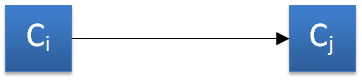
\includegraphics{Figs/noNervousSystem.png}
	\caption{Relationship between the components of an organism without a nervous system.}
	\label{fig:noNervousSystem}
\end{figure}
%\vspace{-0.18cm}
\subsection{Origin of Nervous Systems} The evolution of nervous systems in organisms dates back to the development of primitive electrical signalling in eukaryotes, using calcium action potentials\footnote{See any textbook on evolutionary biology.} and sodium channels \cite{Liebeskind31052011}:

\begin{emquote}
	Voltage-dependent sodium channels are believed to have evolved from calcium channels at the origin of the nervous system.
\end{emquote}

These sodium channels predated modern-day neurons, but served the same fundamental purpose of acting as control systems. We can readily conceive the benefits of imparting a control system onto an organism with the following thought experiment: let us imagine a microscopic organism without any sort of nervous system --- all of its behaviour is hard-coded and mechanical. It can take in nutrients through its cell walls or through an opening; parts of it can contract or expand in response to stimuli like light or pressure; homeostatic conditions can influence its chemistry. Figure~\ref{fig:noNervousSystem} shows this schema: if we enumerate the constituent parts or {\em components} of an organism as $\{C_1,\dots,C_n\}$, the organism's behavior is caused by signals being sent between $C_i$ and $C_j$ (the case $i=j$ is possible). Such an organism suffers from three disadvantages: (a) reactions are localized, as two of its components might be too far apart to communicate in a timely manner or at all; (b) its repertoire of behaviours is necessarily simple and (c) it is not very adaptable.

Precursors to nervous systems ameliorated (a) first via action potentials, which were intracellular electrical signals \cite{Liebeskind31052011} (emphasis mine):
\begin{emquote}
Another key animal innovation was the nervous system, which is present in all but a few animals (i.e., sponges and placozoans). {\em Rapid, specific, long-distance communication among excitable cells} is achieved in bilaterian animals and a few jellyfish (cnidarians) through the use of action potentials (APs) in neurons generated by voltage-dependent sodium (Na$_\mathrm{v}$) channels. Voltage dependent calcium (Ca$_\mathrm{v}$) channels evolved in single-celled eukaryotes and were used for intracellular signaling. {\em It has been hypothesized that Na$_v$ channels were derived from Ca$_v$ channels at the origin of the nervous system} \textsf{[the results in the paper support the hypothesis]} (3), thereby conferring the ability to conduct action potentials without interfering with intracellular calcium. This view was reinforced by the apparent lack of sodium currents in sponges (4).
\end{emquote}

The introduction of dedicated, long-distance\footnote{The term ``long-distance'' may very well mean ``long-distance within a single cell''. Franti\v{s}ek and Mancuso argue in {\em Deep evolutionary origins of neurobiology: Turning the essence of ``neural'' upside-down} \cite{frantisek} that neural analogues already existed in prokaryotes (bacteria and archaea; organisms without cell walls and nuclei) and unicellular eukaryotes.} signalling cells between parts of an organism created the possibility of not only transmitting, but also modifying information. The moment an organism's parts do not communicate directly biochemically/mechanically, but over transmissions lines, evolutionary processes acting upon these lines are able to mutate them so that they change the signals. The first changes might consist of amplifying, diminishing, or distributing signals. Over time, the nerves may come to act as transducers on the stream of signals; in some rudimentary sense, they may begin to compute functions. Schematically, we see this in Figure~\ref{fig:nervousSystem}, where a function $F$ is interposed between two components. Not all components of an organism are created equal, of course. The first and most important use of nerve cells was the communication between sensory organs and the movement apparatus of the organism, and the bulk of nerve cells were located close to the sensory organs, where they processed information. A mere handful of neurons are not able to compute much, but they must have conferred considerable advantage to their owners.

\begin{figure}
	\centering
	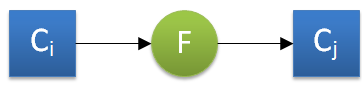
\includegraphics{Figs/nervousSystem.png}
	\caption{Relationship between the components of an organism possessing a nervous system. $F$ can be understood as a simple signal transformer or a central coordinating mechanism.}
	\label{fig:nervousSystem}
\end{figure}

The history of these developments is not entirely clear, but action potentials are present in all animals (with the exception of sponges) and in plants \cite{Leys01051999, PCE:PCE1614}. 
A step up from mere stream transducers are the nerve nets that permeate the entire bodies of cnedaria (jellyfish) and the nerve cords that run along the bodies of bilateria (animals with left and right sides). In Figures~\ref{fig:animalia2} and \ref{fig:animalia} we see them in the phylogeny of the kingdom animalia. Both can process signals in a sophisticated way, and enable the performing of varieties of complex tasks, although the sets vary widely from species to species.

\begin{figure}
	\centering
	\begin{subfigure}[t]{0.30\textwidth}
		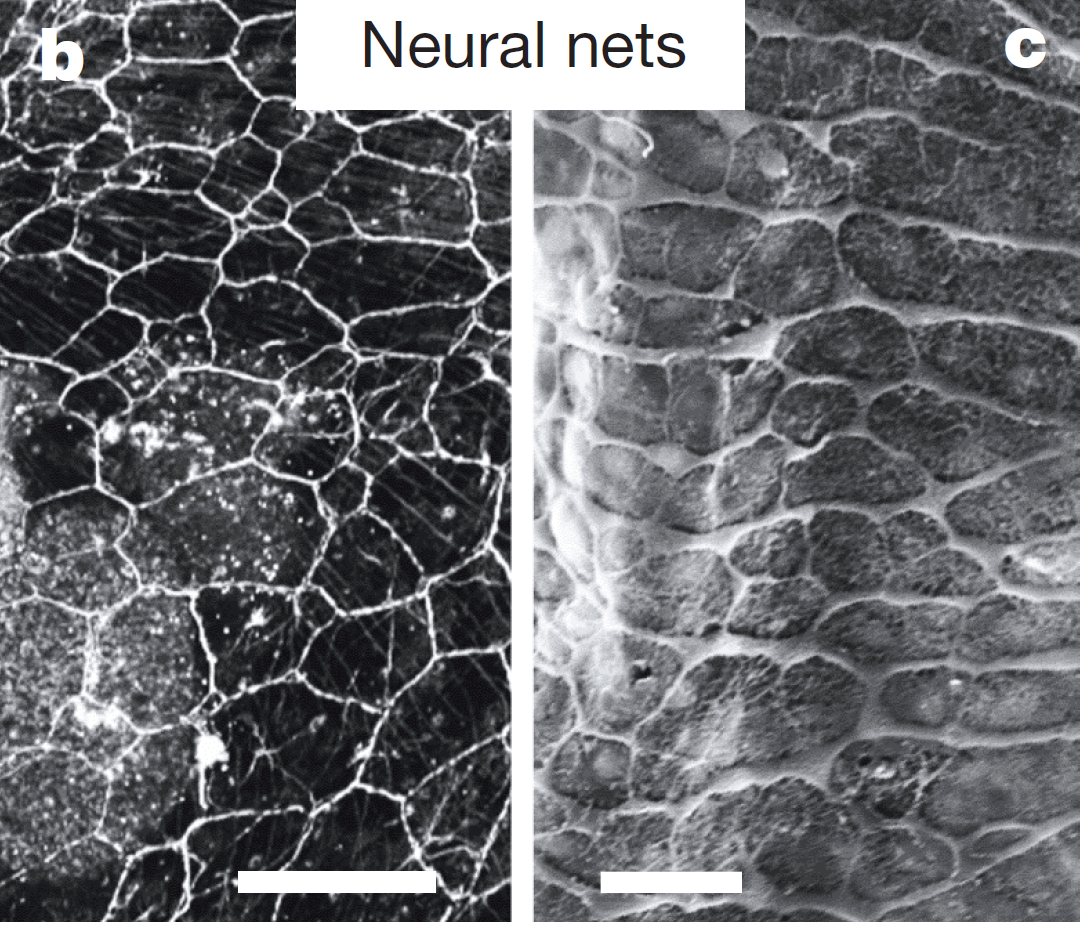
\includegraphics[width=\textwidth]{Figs/neuralNet.png}
		\caption{Nerve nets in ctenaphora.}
		\label{fig:nerveNets}
	\end{subfigure}
	\begin{subfigure}[t]{0.65\textwidth}
		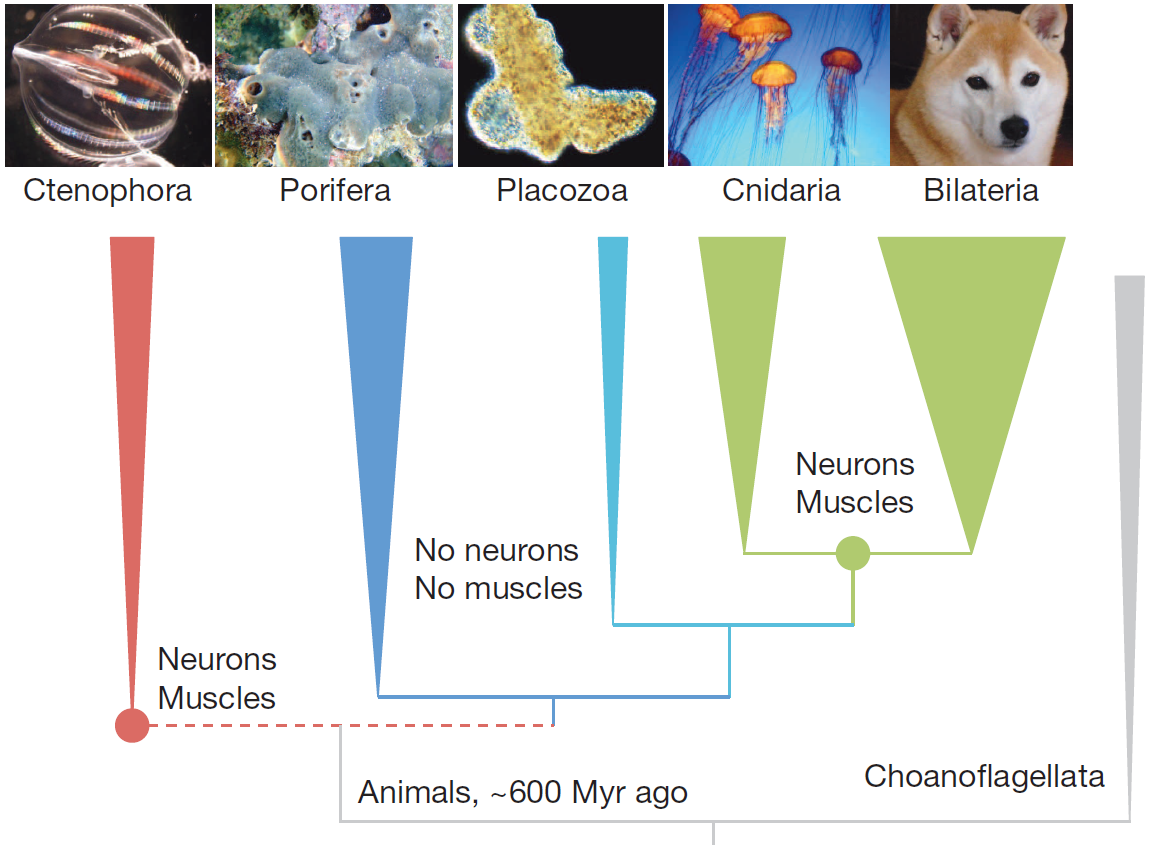
\includegraphics[width=\textwidth]{Figs/animalia3.png}
		\caption{Phyolgeny of the animalia. Even Ctenophores, macroscopic marine invertebrates which predate both jellyfish and bilateria, have nervous systems in the form of distributed nerve nets.}
		\label{fig:animalia2}
	\end{subfigure}
	\caption{Nevre nets and phylogeny of animalia. From {\em {T}he ctenophore genome and the evolutionary origins of neural systems} \cite[p. 100]{animalia2}.}
\end{figure}

\begin{figure}
	\centering
	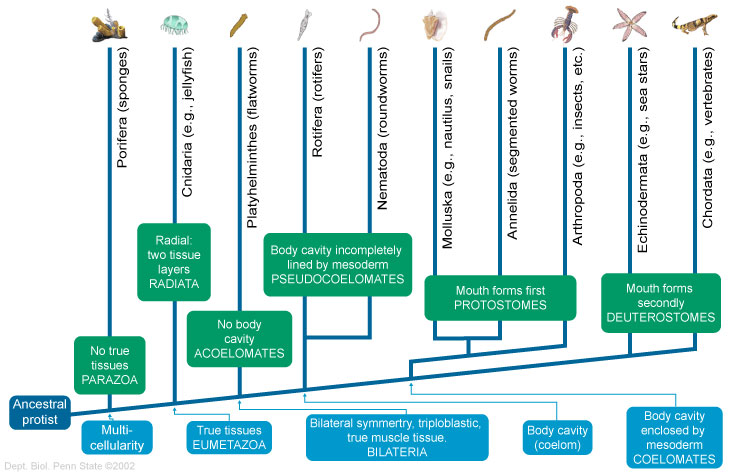
\includegraphics[width=0.8\textwidth]{Figs/animalia.jpg}
	\caption{Phyolgeny of the animalia. Note the cnidaria and bilateria; both of these have types of nervous systems. From {\em Animals I -- An Overview of Phylogeny and Diversity} \cite{animalia}.}
	\label{fig:animalia}
\end{figure}

\begin{figure}
	\centering
	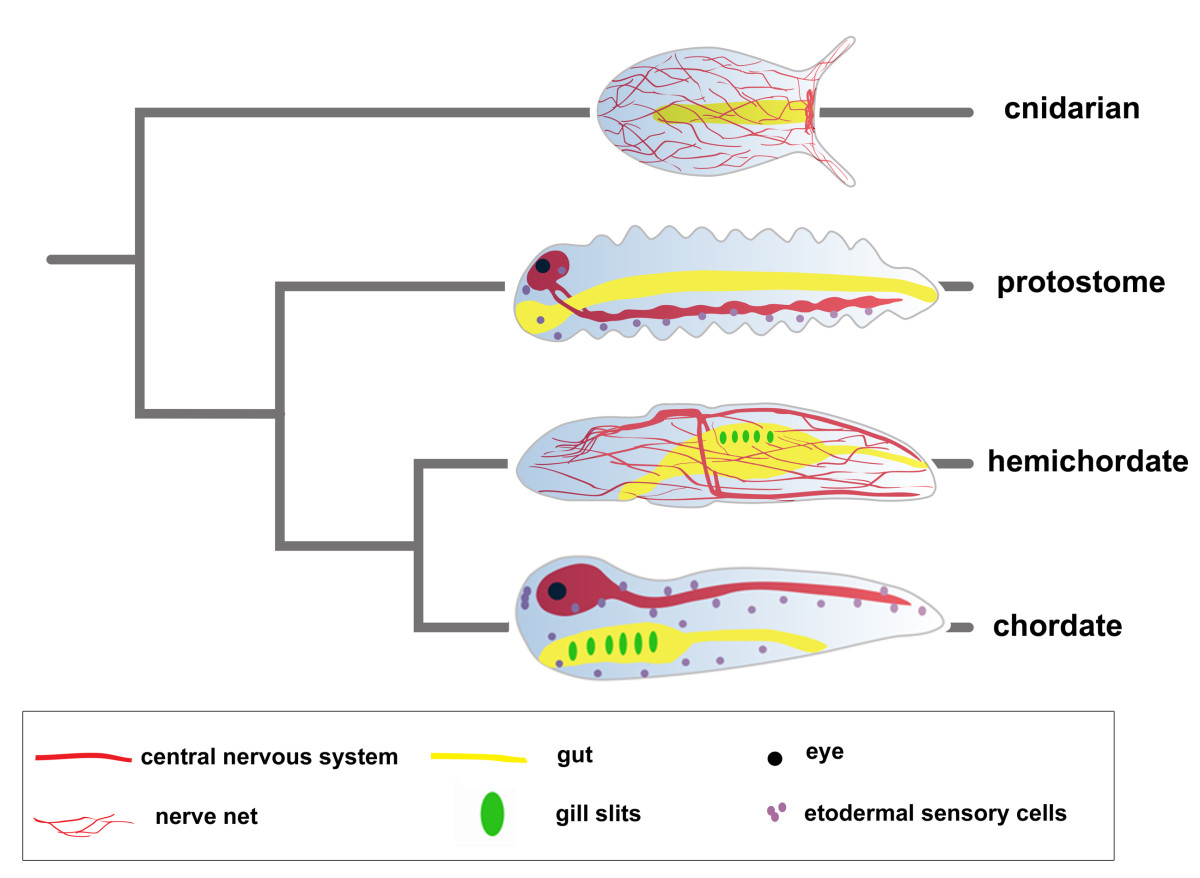
\includegraphics[width=0.8\textwidth]{Figs/chordata.jpg}
	\caption{Body plans for metazoans. The bottom three items are all bilateria and all have nerve cords of some kinds, but only the bottommost (chordates) have a dorsal (upper) nerve cord. Vertebrates are a subphylum of the chordata. From {\em Evolution of bilaterian central nervous systems: a single origin?} \cite[p. 3]{chordata}.}
	\label{fig:chordata}
\end{figure}

\paragraph{Central nerve cord and cephalisation.} Nerve nets, while interesting, are not our aim. Unlike jellyfish, bilateria have a central nerve cord which runs from their front to their back. At various points alongside the cord, we find ganglions --- thickenings containing larger amounts of nerve bundles. In all animals but worms, the frontal ganglion further thickened until it came to contain the overwhelming majority of the organism's neurons --- forming the head. While substantial neural activity was occurring before this time, it is only here that it becomes to proper to speak of brains, and where we can begin to analyse macroscopic structures like lobes.

\begin{figure}
	\centering
	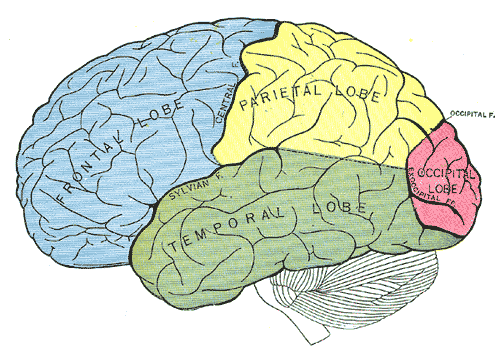
\includegraphics[width=0.65\textwidth]{Figs/brain.png}
	\caption{Illustration of the cerebrum with lobes shown. Hidden: limbic lobe, insular cortex. From {\em Anatomy of the human body} \cite[Fig. 728]{graysAnatomy}.}
	\label{fig:brain}
\end{figure}

Very briefly: vertebrate brains are subdivided into hinbrain, midbrain, and forebrain, having evolved in this order. The forebrain (cerebrum) is responsible for all higher functons and is again divided into six lobes, which we see in Figure~\ref{fig:brain}. The functions performed by these lobes are not precisely understood, but a number can be clearly associated to one lobe. The frontal lobe, for instance, is responsible of conscious thought; the temporal lobe processes auditory and olfactory signals; the occipital lobe deals with sights.\footnote{Interestingly, the occipital lobe is at the {\em back} of the head.} While some functions, like memory, are not neatly localisable, we can nonetheless see in the anatomy of vertebrate and mammalian brains the accruing of large groups of functions: motor control, smell, hearing, sight, reason, emotions. The question of organisation remains, however: it is one thing to say that we have hearing and smell, but what, if anything, ties these experiences together? We, after all, perceive the data from all our senses as one integrated experience. Here, views diverge. The common-sense belief is that we simply have one, indivisible consciousness. Such a view would implicate the frontal lobe as an central organising unit, without which an organism, even if it could smell or see, would not consciously do so. Minsky, Sloman, and Dennett argue persuasively, but speculatively, against this view in their works \cite{emotionMachine,societyOfMind,sloman1991, dennett1991}. They differ on the details, but all agree that the unified consciousness is an illusion; that it is not a single ``I am''-thing gathering raw data, but a dispersed locus of experiences that we merely perceive as immediate.\footnote{Dennett criticises the idea of a \caps{consciousness-thing} with the concept of the ``Cartesian theater'' \cite{dennett1991}. According to him, positing that there is such a thing in our brains, and that it observes all other brain functions, is fundamentally problematic: if there is such a sort of homunculus in our heads that, say, sees the result the output of visual processing in the manner in which one would see a film, then how its visual perception work? Is there yet another a homunculus inside the homunculus that interprets visual information? Such a view implies either an infinite regress, or the algorithmic inexplicability of some part of the brain.} In this view, the frontal lobe, while still instrumental, would not be the only contributor. All other regions of at least the cerebrum would contribute in some way to the organism's conscious experience. An animal without a frontal lobe would not be conscious in the same way as we are, but it would not be utterly blind either --- it would already have some dim awareness of its existence; some rudimentary ``I am'' that we can hardly imagine would already be present in it. To quote Sloman (emphasis mine):\footnote{The quotation appears in {\em The Emotion Machine} \cite[p. 97]{emotionMachine} and Minsky attributes it to a post made by Aaron Sloman in the \texttt{comp.ai.philosophy} newsgroup, but I have been unable to find the original.}
\begin{emquote}
It is not worth asking how to define consciousness, how to explain it, how it evolved, what its function is, etc., {\em because there's no one thing for which all the answers would be the same. Instead, we have many sub-capabilities, for which the answers are different}: e.g., different kinds of perception, learning, knowledge, attention control, self-monitoring, self-control, etc.
\end{emquote}

\paragraph{Implications.} The point in all this is not to give an detailed summary of evolutionary neurobiology; it is to show that nervous systems are ancient, gradually developed things. They have been shaped by the vicissitudes of hundreds of millions of years, and they could have developed in other ways. They were not planned, as a human would understand to word. If we are to gain headway in piecing together the ``big picture'', we must take these facts to heart, and choose our modelling methods accordingly.

In the abstract of this work, I described the biological and the idealistic approaches as being polar opposites, and this is true as far as engineering is concerned, but in terms of their assumptions, false. They are both idealistic. Neural networks, insofar as their users want to re-create human behaviour, implicitly presuppose an intelligence in neurons that is not there. The comparatively small network is taught to compute some desired function, the hope being that it might thereby come to perform some complex, real-world function like common-sense reasoning. In principle, this strategy could work, but in practice, it is unrealistic --- the environment in which real organisms had to succeed was the planet's ecosphere; billions upon billions of nervous systems of all complexities were run over millions of years; nervous systems died off and were re-created from scratch by genes. It is therefore entirely unreasonable to assume that neural network, trained against an objective function over a period of hours or days could re-create the function a biological organism, unless one were to suppose that there is some inherent quality in neurons that strives for such; that groups of cells somehow {\em wish} to organize themselves into specific configurations in which they are able to perform activities we would call ``cognition''. 

All this being said, we should not confuse criticism of the suitability of a method for a specific purpose with criticism of its suitability for any purpose. Neural networks have proven useful in understanding mental activity at small scales; both they and the symbolic/logic-based approaches have had a myriad of industrial applications. From this, however, it does not follow that we can build genuinely intelligent agents with them. Our only means of doing that (the only means that remain) is to laboriously unravel the developmental history of animal brains, step by step, making sense of each development in context. Where empirical data are not available, we at least have to hypothesize how things could plausibly have happened. To day, structural and genetic analyses have been done (via genetic sequencing and MRI), but they do not deliver sufficiently detailed data. Such methods are rather akin to measuring voltages and task time in a PC --- they do tell us something, but an observer would never infer the existence of e.g. compilers, call stacks, or type systems from such observations. For an understanding of the brain so specific that we can re-implement it in a computer, we will need currently non-existent and not-conceived-of technology. Until that day --- and this will be the main thrust of this thesis --- guesswork will have to suffice.

\subsection{Ways of Adaptation}

After the philosophical groundwork and biological basics, let us describe possible means by which nervous systems can change and acquire new features. We begin with the observation that the existence of neuron bundles between parts of an organism is analogous to a loose coupling of components in a software systems. By having intermediaries that take over the task of communication, selection pressure can produce more and more complex functions, since it no longer has to act upon the body parts that send various signals, but change the nervous system that processes these signals instead. As example: pain receptors, muscles fibres, and the optical nerve have been unchanged for quite some time, long pre-dating the human species, but more recent brain developments have given us the ability to utilise them in novel ways --- by providing a rich mental experience of suffering, playing instruments, and mentally rotating objects, respectively. Manipulating the software is far easier and more quickly done than doing so with the hardware, so to speak.

Having said that, the changes still have to have occurred incrementally. Even if a nervous system can change quickly (for evolutionary timescales), it still has change in tiny steps. We shall leave the matter that for the time being, but, as we will discuss later, this simple fact has profound computational consequences that are seldom thematised in discourse on this matter. 

Let us return to the consideration of primitive life forms. We can imagine the malleable neuron bundles of such ancient organisms changing in a variety of ways in the face of selection pressure: when the environment required it, they could, after several generations, start to compute different or more elaborate functions. An organism which had had developed in an environment where food was abundant in bright places and which had now found itself in darkness would have benefited from a variety of plausible changes, such as
\begin{itemize}
	\item an inversion of its light-seeking behaviour,
	\item switching off its metabolism in light places to conserve energy,
	\item accelerating its metabolism in dark places to make better use of the food there.
\end{itemize}

Of course, other changes would have also been possible, such as the metabolization of different food sources,\footnote{A current-day example is given by nylon-eating bacteria, which have developed in the last century and which now have an abundant food source and no competition.} but we can see how the aforementioned three could have been effected through mutations in a simple nervous system. For a system to permit such mutations, it must be far more robust than most products of human engineering, however. If one were to take out a piston in a car or replace a cogwheel in a mechanical clock with a differently sized one, the machine would, in most cases, simply break. In all others, it would catastrophically malfunction. Machines are designed to fit together perfectly and their complexity tends to be irreducible. Even software, which is more readily changed, is easily broken by small-scale tinkering.

When discussing how they can evolve and, in particular, {\em evolve to perform new tasks} and not just variations on old ones, explanations are again constrained by two criteria: (a) the change has to be small, or at least have a small cause\footnote{The effect does not have to be small --- changes in single genes can switch entire components on or off. The MYH16 gene, which is present in non-human primates but has been switched off in humans, is an example. In us, its disabling lead to a drastic reduction in the size of jaw muscles and a corresponding increase in brain size~\cite{carroll2005}. Nonetheless, such events are rare and not the main drivers of evolution.} and (b) each change must be beneficial in the short term.\footnote{Caveats apply: if the selection pressure on a group of organisms is not too strong, changes which may be sub-optimal but perhaps beneficial at some later point may spread, and non-selective processes like genetic drift can also play a role.} Something that we would conventionally recognize as a program, something which has precise notions like "instruction" and "call structure" is probably not suited to this pattern of changes.\footnote{Cf. evolutionary program generation, in which expression trees mutated. I charge that such algorithms are not adequate models of what happened in the evolution of our brains.} Instead, we ought to imagine the brain as a mesh of computation in which functions are computed cumulatively, so that small changes in neural structure only lead to small changes in output.

To illustrate this, we can look at a simple neural network in Figure~\ref{fig:neuralNetwork}, with a marked node $N_x$. Figure~\ref{fig:unlikelyEvolution} shows an unlikely change scenario in which some new component/function is cleanly grafted onto the system. Figures~\ref{fig:likelyEvolution} and \ref{fig:copyEvolution} then show two more likely scenarios: in the first a mutation causes $N_x$ to be split and the new nodes take over some of its connections. In the second, a larger component is accidentally copied as-is and, over time, is moulded to do something useful.\footnote{Such copies can be caused by mutations and are known to happen with some frequency in nature.} In time, new functions can thus grow into the system, but never in the manner in which, say, an engineer would implement a new feature. 

\begin{figure}
	\centering
	\begin{subfigure}[t]{0.45\textwidth}
		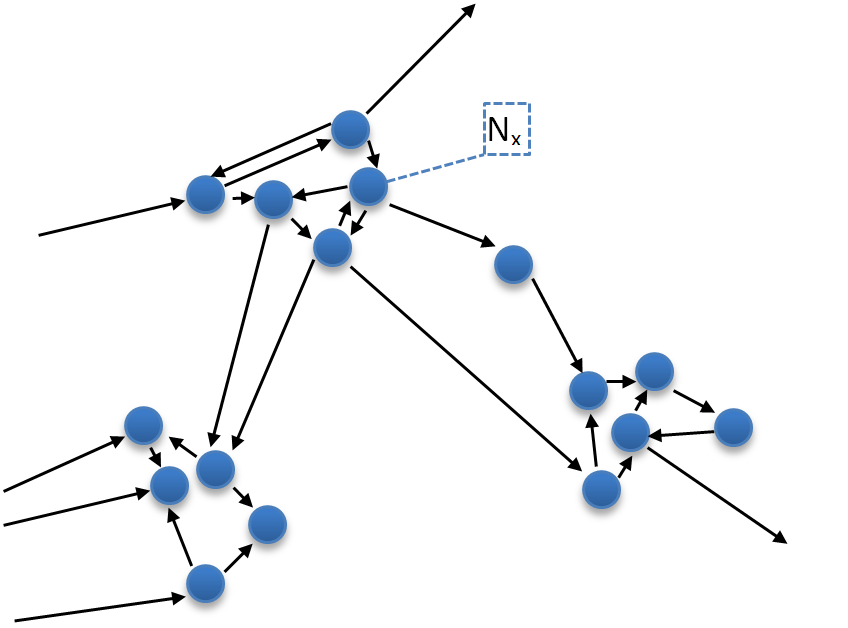
\includegraphics[width=\textwidth]{Figs/neuralNetwork.png}
		\caption{A simple neural network.}
		\label{fig:neuralNetwork}
	\end{subfigure}
	\begin{subfigure}[t]{0.45\textwidth}
		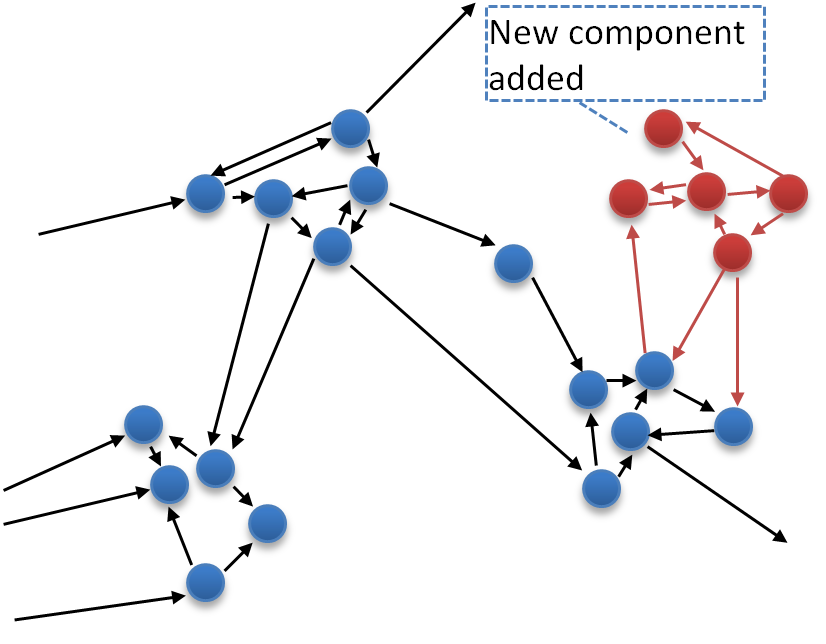
\includegraphics[width=\textwidth]{Figs/unlikelyEvolution.png}
		\caption{An unlikely change scenario in which new, discernible components are grafted on from whole cloth.}
		\label{fig:unlikelyEvolution}
	\end{subfigure}
	\begin{subfigure}[t]{0.45\textwidth}
		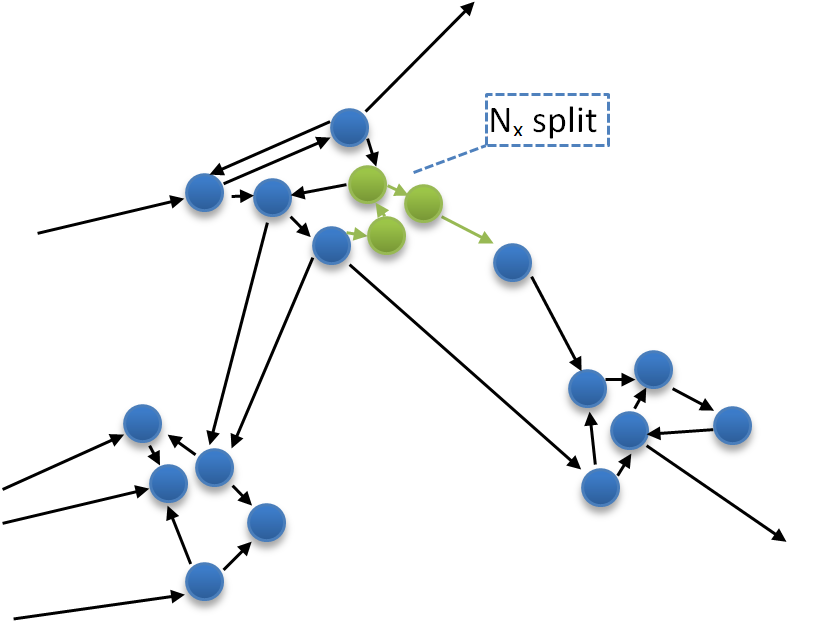
\includegraphics[width=\textwidth]{Figs/likelyEvolution.png}
		\caption{A more likely change scenario in which one part is split into three but where the overall shape of the network is not appreciably altered.}
		\label{fig:likelyEvolution}
	\end{subfigure}
	\begin{subfigure}[t]{0.49\textwidth}
		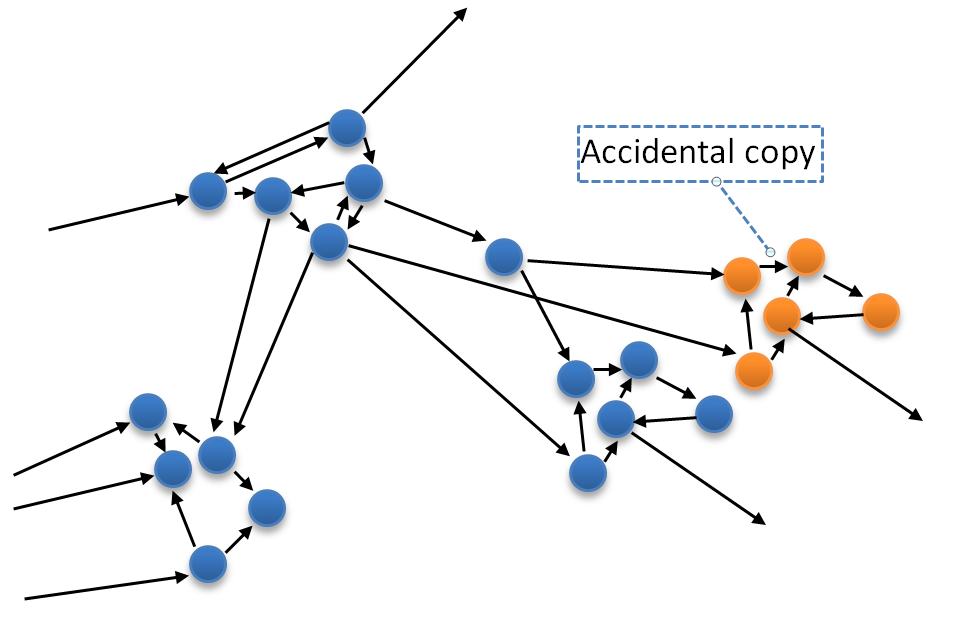
\includegraphics[width=\textwidth]{Figs/copyEvolution.png}
		\caption{A second change scenario in which an entire component is accidentally copied. While the resultant change is large, a small genetic mutation can cause it.}
		\label{fig:copyEvolution}
	\end{subfigure}
	\caption{Means of change in neural networks.}
\end{figure}

\paragraph{Sloman's brain.} One might ask what the relationship between the gradual growth of neural bundles and the observed, large-scale functions in the brain is. We have now supposed at some length that the organisation is not neat, but the question remains whether we can speak of an organisation at all (even a messy one). In {\em Beyond shallow models of emotion} \cite[p. 8]{sloman2000}, Sloman illustrates the possible chaotic organisation of brain with Figure~\ref{fig:slomanBrain}, conjecturing that it might be a jumble of parts that just happen to work together:

\begin{emquote}
	Any observed behaviour might be produced by an unintelligibly tangled and non-modular architecture. (Rectangles represent information stores and buffers, ovals represent processing
	units, and arrows represent flow of information, including control signals.)
\end{emquote}

\begin{figure}
	\centering
	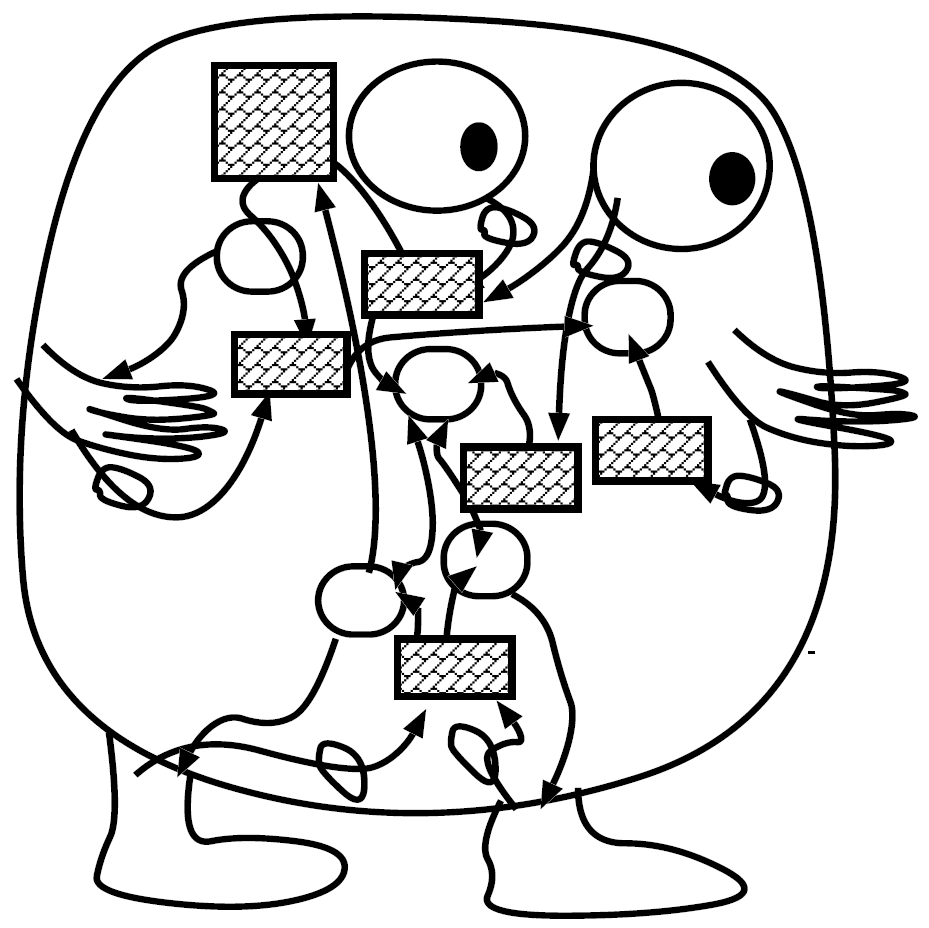
\includegraphics[width=0.6\textwidth]{Figs/slomanBrain.png}
	\caption{Sloman's illustration of the brain as an ``unstructured mess''.}
	\label{fig:slomanBrain}
\end{figure}

This strikes me as a cheery optimism, if anything; one that presupposes that there even are such things as information stores and control signals. The actual situation is, in all likelihood, a far worse one: it is not just different programs that are run in the brain, but entire different models of computation, with the same pattern of activity being interpreted simultaneously in more than one way.
Today, we can scarcely imagine how such an ``architecture'' would work, let alone how one would program --- but if we really want to create genuinely animal intelligences, we will have to find out. Sloman himself admits to the difficulty of gaining understanding of the workings in {\em What Sort of Control System Is Able to Have a Personality?} \cite[p. 6, Section 9 ``Is the task too hard?'']{sloman1997}:
\begin{emquote}
Given the enormous diversity in both design space and niche space and our limited understanding of both, one reaction is extreme pessimism regarding our ability to gain significant insights.
\end{emquote}
The following remedy is offered:
\begin{emquote}
My own attitude is cautious optimism: let us approach the study from many different directions and with many different methodologies and see what we can learn. (\dots)\\
In particular, the Cognition and Affect group at Birmingham has been trying to use a combination of philosophical analysis, critical reflection on shared common sense knowledge about human capabilities, analysis of strength and especially weaknesses in current AI systems, and where appropriate hints from biology, psychology, psychiatry and brain science, to guide a combination of speculation and exploratory implementation (\dots).
\end{emquote}

The methods listed all have their applications, but computational analysis is missing among them. When we talk of psychology, philosophy, and critical reflection, we have already supposed too much; we want to replicate the high-level output of the brain without having explored the mechanism that produces it. In a manner of speaking, we have seen the forest, but do not understand what trees are. If we are to gain the sort of knowledge of brains that we can implement into an AI, we must, empirically, find out about their method of computation. Barring that, we must at least approximate it as far as is practical, and accept that the result will necessarily be an inferior simulacrum.

What, then, is the computational model used in the brain? As yet, nobody knows, and that will stay that way for the foreseeable future. It is very much a guess, but from the concept of slowly growing neural networks (seen in Figures~\ref{fig:neuralNetwork}-\ref{fig:copyEvolution}), one might infer something like the ``active symbol'' hypothesis in Douglas Hofstadter's {\em G\"{o}del Escher Bach}: that patterns of activity form little programs and pieces of data at once; that manipulate other patterns of activation and are manipulated yet other patterns during their lifetime. These are only imperfect analogies, of course. On the coming pages, I shall outline a conceptually compatible white-box model of computation as another, imperfect analogy that will serve as the basis for the model in Sections~\ref{sec:schemaOfCognition}-\ref{sec:mathematicalModel}, and for the implementation of the toy agents in Section-\ref{sec:implementation}.

\section{The Brain as a Collection of White Boxes}\label{sec:whiteBoxModel1}

We now leave the realm of established fact and venture into conjecture. What has been said up to this point has been good, general fact, but it does not suffice for building actual programs. Data on the computational structure of the brain is scarce, thus I will limit myself to positing general, plausible hypotheses about what sorts of structures and loci of computation could have plausibly arisen in it over the course of its evolution. 

A plausible case has been made by Minsky, Sloman, and others (especially in {\em The Emotion Machine} \cite{emotionMachine}) that the brain must possess components in some form. Were it not so, the organ would have long ago succumbed to the innefficiences of its design. As more and more functions are grafted onto a system, the number of interactions between its parts or regions, and therefore the bugs in it, increases. Worse yet, the system becomes brittle: even if, like in a neural network, some accidentally working configuration would have been able to be reached, small changes would surely have upset it again. The part-less system is an evolutionary dead-end from which no improvement is possible, and given how far along our cognition is, it is quite clear that we are not dealing such when we look at our brains.

If we concede that we are dealing with identifiable parts, a second question arises: how do these parts communicate? I would like to deal with with this question in some detail. In the literature, this issue is often glossed over --- in diagrams, one frequently finds unannotated arrows going between functions; the accompanying texts mention concepts like ``selection'', ''message'', and ``sending'' under the implicit assumption that these are merely primitives in no need of further explanation. When we consider the workings of neurons, however, it is not at all clear how groups of them could put together any sort of complex message, and, once put together, how it would travel, and how another group of neurons could receive and interpret it. Are there dedicated interpreters, akin to compilers and runtimes in computer systems? This is not known. I cautiously propose that it is not so, but we can present plausibly-sounding scenarios for both outcomes:
\begin{itemize}
	\item On the one hand, we may image that, early on, some simple message format developed through, allowing more efficient communication between not quite differentiated regions of a nervous system. Over time, this was extended as more components came into play; these new components would have found it easier to make use of the pre-existing protocol. Larger clusters of parts might have even repeated the process and developed simple, internal message formats for communication among themselves. As an orthogonal development, newly developed components might have performed more abstract duties, using older ones as subsidiaries, if at all. To solve conflicts whenever these new and old parts proposed different solutions to whatever issue the organism faced, some other component could have received inputs from both, and adjudicated. In such way, a hierarchical and layered structure could have come into being --- different layers working at different levels of abstraction, and each component only communicating on an on-basis with others. All in all, the whole system would come to resemble a human-developed program.
	
	\item On the other hand, we could imagine quite a different scenario: suppose that the basic scheme of neurons sitting as growths on the communication lines between components never changed. Their basic task was the modulation of signals, and if some new function was to be grafted into the system, then this would have been achieved by growing more neurons that modulated the signals of their fellow neurons. They would not have opened a communication channel with the existing components, but would have listened in on their activity in the manner of interlopers surreptitiously modifying messages. Since neurons would have had no reason to hide their activity (as a black box does), this would have been quite easy and straightforward to do. New bundles of functionality could have inserted themselves into the middle of the information flow (enhancing existing functionality, or adding administrative features), before it (providing pre-processing), or after it (providing post-processing, or usage of the output for higher-level tasks). In contrast to above, we concentrate on the {\em process} of software development instead of its product: a human programmer adds functions one at a time, here and there, extending and refining functionality where fancy strikes or necessity requires.
\end{itemize}

One could thus call the first scenario the \caps{product-oriented view} and the second the \caps{ process-oriented view}: the first looks at the end product of a development, the second posits that the very process of that development, fossilized, is present in the end product.

Evidence is scarce and equivocal for both. In fact, it need not even be the case that they form a dichotomy: we might just as well speculate, for instance, that the second is the low-level reality, but that the first emerged from over time due to the efficiency of its design. The components could be fuzzy, to some degree. We could also posit that the first one ``degenerated'' into the second one; that a formal system is emulating an informal one because of the latter's greater versatility and dynamism.

For the rest of the thesis, I will explore the second of the above two hypotheses, not necessarily because I firmly believe it to be true, but rather because the first one has been tried for some time, and has so far not produced a general AI.

\paragraph{Practical abstraction.} While such a white-box model, and the hypothesizing that preceded it, are conceptually useful, a mesh of gradually grown patterns does not lend itself to implementation in a program. We do not have the capability of faithfully pouring the structure of the human brain into a computerized mould just yet, but, for the time being, we may opt for the next best thing and take cues from it in the hopes of improving our imitations.

\begin{figure}
	\centering
	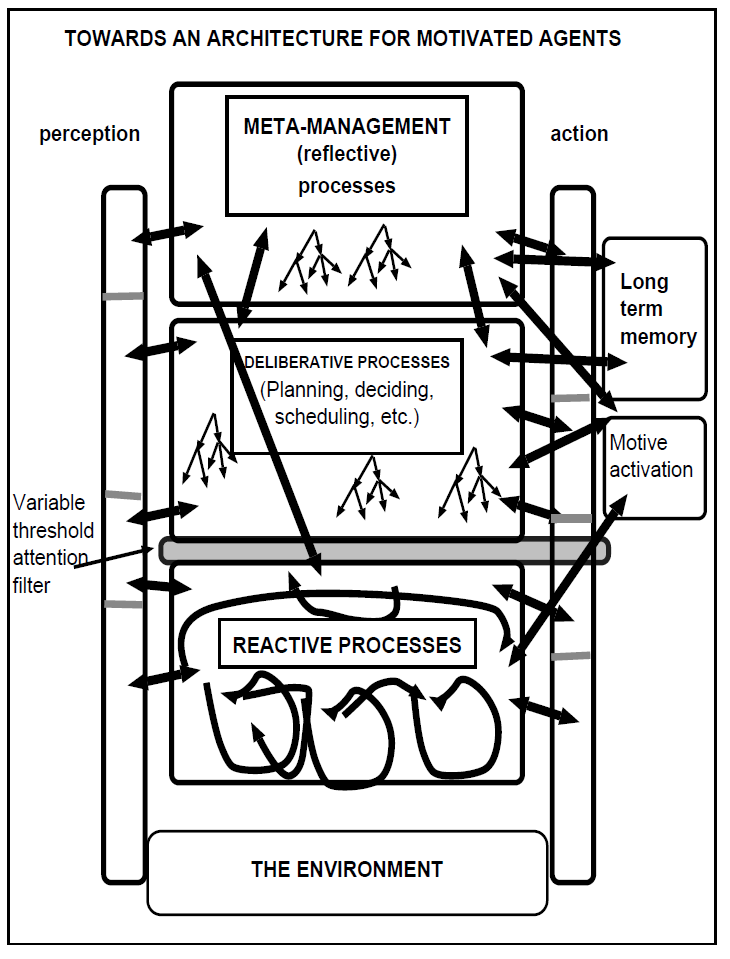
\includegraphics[width=0.8\textwidth]{Figs/slomanSystem.png}
	\caption{Architecture for motivated agents. From \cite[p. 10]{sloman1997}}
	\label{fig:slomanSystem}
\end{figure}

Therefore, I will present a simplified model which, while attempting to remain true to the conceptual view, will, pragmatically, contain discrete functions and components. The white-box nature of brain activity will be emulated by a message-passing scheme in which messages model the internal activity of components. Instead of each component blindly acting in some fashion on the activity of another, components will have explicit parsers and interpreters and later, these will be further simplified into localized message formats and tagging, for the sake of easy implementation.
This effort is guided by the same thought as Sloman's cognitive architecture see in Figure~\ref{fig:slomanSystem}. It is not a truly accurate representation of the brain and it does not claim to be, but it is {\em something like it}; something that is close, and good, enough. We will meet this cognitive architecture again later, but for now, we move on to the description of neural components.

%While some form interpretation surely must happen in one or more places, it is implausible to suppose that there is one agreed-upon message format, or one programming language that all parts use. 
%
%
%The facts and processes of the previous subsection are relatively uncontroversial and can be found reiterated in any textbook on the evolution of nervous systems. The functional structure and the model of computation used in the brain, however, are not well understood. FMRI and similar brain imagining techniques, while invaluable, give only rough impressions about the neural correlates of certain forms of cognition and do not give fine-grained insight into its structure. As such, the model I shall describe in the following paragraphs is a conjecture. The implication of such an evolutionary viewpoint, I conjecture in this document, is that brain functions don't ``just appear'', but are rather the result of small changes and the recombination of pre-existing parts. This, in turn, informs the plausibility of various possible brain architectures. It becomes unlikely that the brain should be a collection of neatly delineated functions, or that it should have certain coordinating units or universal message formats for communication between components. The reason for this is that administrative mechanism confer little evolutionary benefit on their own, and do not confer it gradually: the imposition of a central coordinating mechanism on a pre-existing mesh of neurons would necessitate the complete reorganisation of such, and the abandonment of the previous communication channels in favour centralized coordination. The same objections can be raised against a universal or even a local message format. Moreover, such mechanisms require substantial changes in the organism with no obvious or immediate advantage.
%
%These objections do not contradict the existence of macroscopic structures in the brain, dedicated to certain tasks. The development and adaptation of such remains entirely plausible. They do, however, give insight into the pattern of processing inside such structures, which is often simply regarded as atomic or replicated in computers as if it were a conventional engineering product.
%
%Instead of a rigidly ordered brain with central organisation and large, discrete, and highly complex features like ``sight'' or ``reason'' which function like ready-made black boxes, to be plugged in at will, I propose a decentralized white-box architecture composed of simple parts: first, every component, while perhaps sophisticated, is conceptually simple. Second, communication between different components is not performed in the function-call pattern of computer programs, but rather by one component listening in on the activity of another. Since there is, inherently, no mechanism of function abstraction in neural systems, it stands to reason that the most likely way for new functions to develop is for additional neurons to modulate the activity of others. In such a scheme, a visual perception component does not have to know which other components will consume its output (or rather, listen on its activity); changes which affect agent activity in useful ways based on the visual data can occur gradually and, over time, become large enough to count as components in their own right.

	
	\chapter{Overall Component Model}\label{ch:componentModel}
	
	\section{Components as White Boxes}\label{sec:whiteBoxModel2}

We can imagine the components of the mind as white boxes which inform other components by their very functioning --- however, this does not lend itself to easy implementation. Instead, we can emulate this behaviour via a \emph{message space}, from which individual components take their input and into which they put their output. A \emph{component} is then a local processing unit which continuously scans the message space, running messages through its \emph{filter}. If the filter detects a relevant message, it is then passed to the \emph{interpreter}, which parses the message into the needed format and hands it over to the \emph{processor}. The processor, after having finished, puts its output back into the message space for other components to read. Figure~\ref{fig:global} illustrates this scheme. Note the lack of explicit hierarchical structure and central organising units.

\begin{figure}
	\begin{center}
		\begin{tabular}{l l}
			\toprule
			Symbol & Description\\
			\midrule
			
			\begin{minipage}[t]{0.2\textwidth}
				
\includegraphics[width=80pt]{Figs/legend_proc.png}
			\end{minipage}
			& Processing component\\
			
\includegraphics[width=80pt]{Figs/legend_choice.png} & Choice\\
			
\includegraphics[width=50pt]{Figs/legend_container.png} & Data container (Queue, List, etc.)\\
			
\includegraphics[width=50pt]{Figs/legend_data.png} & Data\\
			
\includegraphics[width=30pt]{Figs/legend_generator.png} & Stream generator\\
			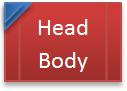
\includegraphics[width=50pt]{Figs/legend_imaginary.png} & Counterfactual (imaginary) data\\
			\bottomrule
		\end{tabular}
	\end{center}
	\caption{Notation for the diagrams in this and the following sections.}
	\label{fig:diagramNotation}
\end{figure}
%
\begin{figure}[!h]
	\centering
	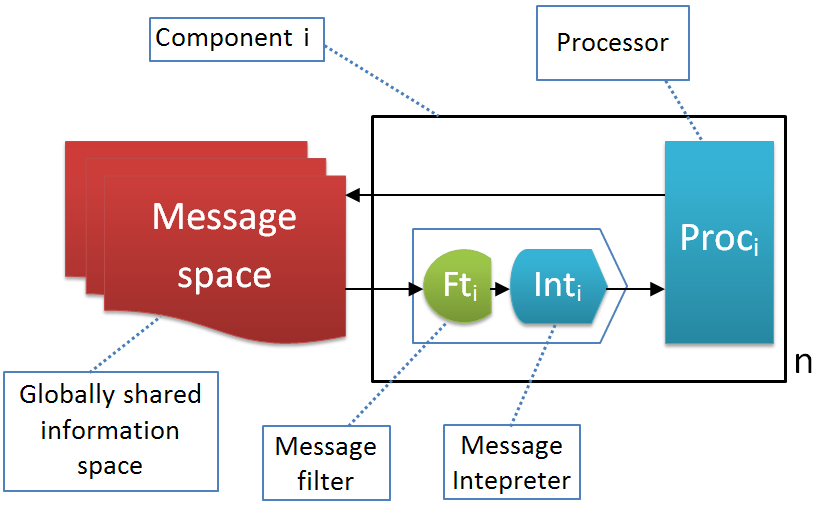
\includegraphics[width=400pt]{Figs/global.png}
	\caption{Global neural architecture.}
	\label{fig:global}
\end{figure}

However, as we will show in the next section, this model is generic enough to accommodate such special-purpose structures. Figure~\ref{fig:global} shows the message-passing scheme, but it also specifies a graph in which the nodes are the components and fixed, while the edges are the accepted messages and are determined by the nodes; through their filters, components control the shape of the graph. By imposing invariants on these filters, we can have the graph take any shape we desire. In particular, we can model the kinds of structures that occur in many other cognitive models and in empirical research: central organisers, sequences of components (``pipelines''), localized messages affecting only a small part of the mind, a component reading its own messages, loops and iterative messages between two or more components et cetera.

\pagebreak

\paragraph{Messages.}

We may now ask how such messages between components are structured. Here, I make two empirical claims:
\begin{enumerate}
	\item messages have a priority and
	\item they are effectively unstructured.
\end{enumerate}

\begin{figure}[!h]
	\centering
	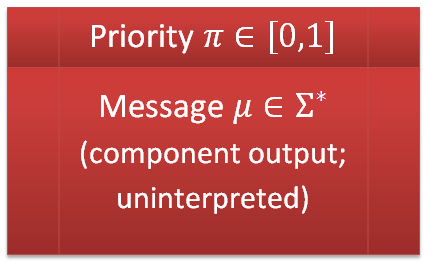
\includegraphics[width=150pt]{Figs/message.png}
	\caption{Structure of a neural message.}
	\label{fig:message}
\end{figure}

To the best of my knowledge, the veracity of either has thus far not been determined by neuroscience. For the first, Marvin Minsky's ``The Emotion Machine'' provides some circumstantial evidence \cite[p.\ 222]{emotionMachine}:

\begin{quote}
	Of course, when one activates two or more Critics or Selectors, this is likely to cause some conflicts, because two different resources might try to turn on a third resource both {\em on} and {\em off}. To deal with this, we could design the system to use various policies like these:
	
	\begin{enumerate}
		\item Choose the resource with the highest priority.
		\item Choose the one that is most strongly aroused.
		\item Choose the one that gives the most specific advice.
		\item Have them all compete in some ``marketplace''.
	\end{enumerate}
\end{quote}

The selection strategies Minsky lists imply that there is some mechanism in the brain to determine the urgency of a signal. While it is possible that higher brain functions like reasoning or affect make an additional, rational evaluation, sensations like intense pain, bright lights, or great sadness can likely be communicated most easily by the appropriate components causing a flood of activity which, by its very intensity, informs other components of the urgency of their messages.

The second claim --- that messages are essentially unstructured --- means that there is no common, agreed-upon format in which they are stored. In addition to the evolutionary implausibility of such a format being created, an unstructured message format is in line with the white-box nature of components: since components merely ``listen in'' on others, and since each components will have its own pattern of activity, a listener would simply have to try and make sense of this activity as best it could. The proposed structure of messages is thus shown in Figure~\ref{fig:message}: every message comprises a priority header, together with an unstructured body which, for our purposes, is simply a string of bits.

\paragraph{Filters.} Before a component can respond to a message by another, such a message must be assessed for the presence of relevant information. Conceptually, this happens via a \emph{filter} in each component, which pattern-matches incoming messages and, if a certain threshold is reached, signals relevance and hands the message over the \emph{interpreter} for parsing. Figure~\ref{fig:filter} shows such a filter: it is composed of a directed graph of nodes, and a node is activated if it detects some specific content in the message. Nodes, in turn, are connected via edges of strength $\in [0,1]$. When a node is activated, it sends a charge proportional to the strength of its link to its neighbours, contributing to their activation as well. Some nodes are marked as {\em output nodes}; if enough such output nodes become activated, the message is deemed to be sufficiently relevant. This model of filters is inspired by the {\em spiking neural P Systems} of Georghe Pa\u{u}n et al. (\cite[p.\ 337]{membraneComputing} and \cite{spikingNeural}), in which charges sent along directed graphs of neurons are used to compute functions.

\begin{figure}[!h]
	\centering
	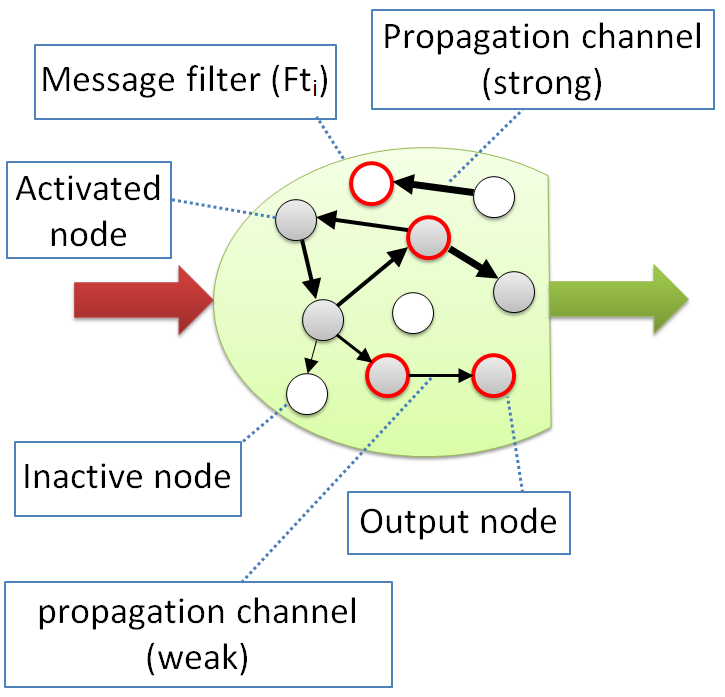
\includegraphics[width=168pt]{Figs/filter.png}
	\caption{A pattern-matching filter for a component $C_i$.}
	\label{fig:filter}
\end{figure}

\section{Mathematical Model}\label{sec:mathematicalModel}

We now create a mathematical model for the description of the architecture. This model will be split into two parts: the structural and the operational semantics. The structural semantics encode the static properties of neural systems, whereas the operational semantics describe the behaviour of such a system at runtime.

\subsection{Preliminaries}\label{sec:mathematicalPreliminaries}

Since the mathematical model is built with implementation in mind, I will use some basic type theory in the coming sections. The following notions are from the $\lambda$-calculus and its attendant type systems; anyone familiar with such can therefore freely skip this section. We will introduce types, type constructors, and their relation to functions, together with a few example types which will come in handy later on. The following can be found in any introduction to type theory and was taken (with simplification) from \cite{Mendler:1988:IDT:913822}, \cite{typeIntroduction2}, and \cite{Jacobs97atutorial}.

\begin{definition}[Syntax: Type]\label{def:type}
	For our purposes, types are defined inductively thus:
	\begin{description}
		\item[Basic type.] $\R$ and $\emptyset$ are types.
		\item[Sum type.] If $\type{T_1},\type{T_2}$ are types, the {\em sum type} $\type{T_1 + T_2}$, is a type. 
		\item[Product type.] If $\type{s}$ is a string and $\type{T_1},\dots,\type{T_n}$ are types, the {\em product type} $\type{s}\ \type{T_1} \dots \type{T_n}$, is a type. A special case is the {\em anonymous product type} \paren{tuple}, where $s=``\langle\rangle"$. There, we just write $\langle\type{T_1},\dots,T_n \rangle$.
		\item[Full application.] If $\type{T_1},\dots,\type{T_n}$ are types and $\allQ{x_1,\dots,x_n} \type{C}$ is a type constructor \paren{see next definition}, then $\type{C\ T_1} \dots \type{T_n}$, is a type.
		\item[$\mu$-abstraction.] If $\type{T}, \type{S}$ are types and $\type{S}$ occurs in $\type{T}$, then $\muQ{\alpha}\type{T}[\type{S}\backslash\alpha]$ \paren{for a fresh variable name $\alpha$} is a type.
	\end{description}
\end{definition}

\begin{definition}[Syntax: Type constructor]\label{def:typeCon}\
	Type constructors are the defined thus:
	\begin{description}
		\item[Base case.] Every type $\type{T}$ is a type constructor.
		\item[Abstraction.] If $\type{C}$ is a type constructor and $\type{T}$ is a type, $\allQ{x} \type{C}[\type{T}\backslash x]$ is a type constructor.
		\item[Sum types.] If $\type{C_1}\dots,\type{C_n}$ are type constructors with $\type{C_i} = \allQ{\vec{X}_i} \type{T_i}$ \paren{$1 \leq i \leq n$}, then $\allQ{\vec{X}_1; \dots; \vec{X}_n} (\type{C_1} + \dots + \type{C_n})$ is a type constructor.
		\item[Partial application.] If $\type{T_1},\dots,\type{T_i}$ \paren{$i < n$} are types and $\allQ{x_1,\dots,x_n} \type{T}$ is a type constructor, then $\allQ{x_{i+1},\dots,x_n} \type{T}[x_1\backslash \type{T_1},\dots,x_i\backslash \type{T_i}]$ is a type constructor.
	\end{description}
\end{definition}

Every type is interpreted as a set of values which are of that type; type constructors are interpreted as universally quantified templates for actual types. Their formal semantics are as follows:

\begin{definition}[Semantics: Type]\label{def:typeSem}
	Let $\type{T}$ be a type. Its interpretation function $\tint(\type{T})$ is defined thus:.
	\begin{description}
		\item[Basic type.] $\R$ is interpreted as the set of real numbers. $\tint(\emptyset) = \{\}$.
		\item[Sum type.] If $\type{T_1}, \type{T_2}$ are types, then $\tint(\type{T_1 + T_2}) = \tint(\type{T_1}) \cup \tint(\type{T_2})$.
		\item[Product type.] If $\type{T_1},\dots,\type{T_n}$ are types and $\type{s}$ is a string, then
		$$
		\tint(\type{s}\ \type{T_1} \dots \type{T_n}) = \left\{
		\begin{array}{l l}
		\{\type{s}\} & \mt{if } n = 0\\
		\{\type{s}\} \times \tint(\type{T_1}) \times \dots \times \tint(\type{T_n}) & \mt{if } n \geq 1.
		\end{array}
		\right.
		$$
		
		\item[Full application.] If $\type{T_1},\dots,\type{T_n}$ are types and $\allQ{x_1,\dots,x_n} \type{C}$ is a type constructor, then
		$$
		\tint(\type{C}\ \type{T_1} \dots \type{T_n}) = \bigcup\limits_{v_1 \in\ \tint(\type{T_1})} \cdots \bigcup\limits_{v_n \in\ \tint(\type{T_n})} \left( \bigcup\limits_{C' \in\ \cint(C)} C'[x_1\backslash v_1,\dots, x_n\backslash v_n] \right).
		$$
		
		\item[$\mu$-abstraction.] If $\muQ{\alpha}\type{T}$ is a type, then $$\tint(\muQ{\alpha}\type{T}) = \tint(\type{T}) \cup \tint(\type{T}[\alpha\backslash\type{T}]) \cup \tint(\type{T}[\alpha\backslash\type{T}][\alpha\backslash\type{T}]) \cup \dots$$
		
		with $\tint(\alpha) = \{\}$.
	\end{description}
\end{definition}

\begin{definition}[Semantics: Type constructor]\label{def:typeConSem}
	The partial interpretation function $\cint$ for type constructors is defined as follows: if $\type{C}$ is a type constructor containing exactly the types $\type{T_1},\dots,\type{T_n}$, then
	$$
	\cint(\type{C}) = \bigcup\limits_{v_1 \in\ \tint(\type{T_1})} \cdots \bigcup\limits_{v_n \in\ \tint(\type{T_n})} \type{C}[\type{T_1}\backslash v_1,\dots,\type{T_n}\backslash v_n].
	$$
\end{definition}

Intuitively, sum types are simply unions, product types are named Cartesian products, and full applications are instantiations of type constructors with all possible values. $\mu$-abstraction represents recursive data types such as lists or trees. Type constructors themselves are just generic types.

Whenever we want to assert that an expression has a specific type, we write:

\begin{notation}[Typed expressions]
	Let $x$ be an expression and $\type{T}$ a type. $x :: \type{T}$ asserts that $x$ has type $\type{T}$.
\end{notation}

Henceforth, by convention, we will write type variables in lower-case and concrete types in upper-case, omitting the explicit $\forall$-blocks. That is, a type like $\allQ{x,y,z} \type{C\ x\ (\N + T_1)\ y\ z}$ will simply be written as $\type{C\ x\ (\N + T_1)\ y\ z}$ and it will be clear that $\type{x}, \type{y}, \type{z}$ are type variables, while $\N, \type{T_1}$ are concrete types. A special kind of type constructor is the function arrow ($\rightarrow$) which induces the function type:

\begin{example}[Function arrow]
	If we take, say, the type $\rightarrow \type{S1}\ \type{S2}$ (a product type with the product types $\type{S1}$ and $\type{S2}$ as arguments) and abstract twice, we get $\allQ{s,t} \rightarrow \type{s}\ \type{t}$. $\rightarrow \type{s}\ \type{t}$ is the type constructor for unary functions from $\type{s}$ to $\type{t}$, also written infix as $\type{s} \rightarrow \type{t}$. Functions with multiple arguments, mapping $\type{t_1},\dots,\type{t_{n-1}}$ to $\type{t_n}$, can be modelled in two ways: either through n-tuples, or through nested function arrows:
	
	$$
	\begin{array}{l}
	\tuple{\type{t_1}, \type{t_2}, \dots \type{t_{n-1}}} \rightarrow \type{t_n}\\
	\type{t_1} \rightarrow (\type{t_2} \rightarrow \dots \rightarrow (\type{t_{n-1}} \rightarrow \type{t_n})\cdots)
	\end{array}
	$$
	
	The first method necessitates that we supply all arguments at once, whereas the second allows them to be given one after another.
\end{example}

\noindent
Function arrows allow the execution of functions in the obvious way:

\begin{definition}[Function application]
	Let $f :: \type{S} \rightarrow \type{T}$ and $x$ be an expression of type $\type{S}$. Then $f\ x$ is an expression of type $\type{T}$. Function application associates to the left, that is: $f\ x_1 \dots x_n = (\cdots((f\ x_1)\ x_2) \dots x_n)$.
\end{definition}

\noindent
We can combine type constructors, sum types, and product types into {\em algebraic data types} (ADTs).

\begin{definition}[Algebraic data type (ADT)]\label{def:ADT}
	Let $\type{s}$ be a string and $\type{C_1},\dots,\type{C_n}$ be type constructors such that $\type{C_i} = \allQ{x_1,\dots,x_n} \type{T_i}$ and $\type{T_i}$ is a named product type with type variables \paren{$1 \leq i \leq n$}. Then $\allQ{x_1,\dots,x_n} (\type{T_i} + \dots + \type{T_n})$ is an ADT. If we want to give a name to an ADT, we write it as $\type{s\ x_1 \dots x_n = T_i + \dots + T_n}$.
\end{definition}

Since an ADT is merely the sum of product types, it is itself a type constructor. If it has no type variables, it is also a type. Next, we define a couple of example ADTs, some of which we will use in the next section.

\begin{example}[$\N$, $\B$, $\Q$, $\C$,  Maybe, Either, List]
	$$
	\begin{array}{l c l}
	\N & = & \muQ{\alpha}\type{Z + S\ \alpha}\\ 
	\B & = & \type{False + True}\\
	\Q & = & \type{Rat}\ \N\ \N\\
	\C & = & \type{Complex}\ \R\ \R\\
	\type{Maybe\ t} & = & \type{Nothing + Just\ t}\\
	\type{Either\ l\ r} & = & \type{Left\ l + Right\ r}\\
	\type{List\ a} & = & \muQ{\alpha}\ \type{Nil + (a : \alpha)}\\
	\end{array}
	$$
	
	$\N$ is the usual Peano definition of natural numbers, with a nullary product type $\type{Z}$ representing zero, and a unary product type $\type{S}$, which allows recursion. $\B$, $\Q$, $\C$ are the sets of Boolean number and rational/complex numbers, respectively, with $\type{False}$ and $\type{True}$ being nullary product types, and with $\type{Rat}\ \N\ \N$ and $\type{Complex}\ \R\ \R$ being binary ones. $\mathtt{Maybe}$ represents an optional value, which may or may not be present. $\mathtt{Either}$ represents a choice between two values, of which either the left or the right one is present, but not both. $\type{List\ a}$ \paren{or just $\type{[a]}$ as a shorthand} denotes a list of values of type $\type{a}$. There, $\type{Nil}$ is the nullary type constructor for an empty list and $\type{:}$ is an infix binary type constructor that stores the head and tail of a list.
\end{example}

\noindent
We also define the usual convenience functions for these types:
$$
\begin{array}{l l}
\begin{array}{r c l}
\field{isJust} & :: & \type{Maybe\ a \rightarrow Bool}\\
\field{isJust}\ m & = & \left\{
\begin{array}{l l}
\type{True} & \mt{if } m = \type{Just}\ x\\
\type{False} & \mt{otherwise}\\
\end{array}
\right.\\
\\
\field{fromJust} & :: & \type{Maybe\ a \rightarrow a}\\
\field{fromJust}\ m & = & \left\{
\begin{array}{l l}
x & \mt{if } m = \type{Just}\ x\\
\bot & \mt{otherwise}\\
\end{array}
\right.\\
\end{array}
&
\begin{array}{r c l}
\field{head} & :: & \type{[a] \rightarrow a}\\
\field{head}\ l & = & \left\{
\begin{array}{l l}
x & \mt{if } l = x:xs\\
\bot & \mt{otherwise}\\
\end{array}
\right.\\
\\
\field{tail} & :: & \type{[a] \rightarrow [a]}\\
\field{tail}\ l & = & \left\{
\begin{array}{l l}
xs & \mt{if } l = x:xs\\
\bot & \mt{otherwise}\\
\end{array}
\right.\\
\end{array}
\end{array}
$$

Definitions~\ref{def:type}--\ref{def:ADT} specify a fragment of System F$_\omega$,\footnote{Specifically, the decidable fragment of System F$_\omega$ without higher kinds and only prenex-polymorphism. That is, type constructors can only take types as arguments and are of the form $\allQ{x_1,\dots,x_n} \type{C}$ for quantifier-free $\type{C}$. This is also called the Hindley-Milner type system. For details, see \cite{barendregt91}.} which is used to type expressions in the lambda calculus. Although System F$_\omega$ is strictly more powerful, our definitions are enough to provide a description language for the data types and functions in the rest of this work.


\subsection{Neural Systems}\label{sec:mathematicalNeuralSystem}

\begin{definition}[Neural component]
	Let $I$ be an index set and let $\type{T}$ be any type. Then, a neural component $C$ with a name from $I$ and message type $\type{T}$ is a four-tuple
	$$
	\tuple{\field{name}, \field{ft}, \field{int}, \field{proc}}
	$$
	where
	\begin{enumerate}
		\item $\field{name} :: I$ is the {\em name} of $C$,
		\item $\field{ft} :: \type{T \rightarrow \B}$ is  called the {\em filter} of $C$,
		\item $\field{int} :: \type{T} \rightarrow \type{Maybe\ T}$ is called the {\em interpreter} of $C$, and
		\item $\field{proc} :: \type{T} \rightarrow \type{T}$ is called the {\em processor} of $C$.
	\end{enumerate}
	
	Formally, the type of $C$ is $\field{Comp}_{\type{T},I}$. As a shorthand, we denote the name, filter, interpreter and processor of a given component $C$ as $\field{name}_C$, $\field{ft}_C$, $\field{int}_C$, $\field{proc}_C$, respectively.
\end{definition}

\noindent
A set of neural components, together with a set of messages, induces a {\em neural system}:

\begin{definition}[Neural system]
	Let $T$ be any type and let $I$ be an index set. Then, a neural system with message type $T$ and component names from $I$ is a tuple
	$$
	\langle \textbf{Co}, \textbf{Me} \rangle
	$$
	where
	\begin{itemize}
		\item $\textbf{Co}$ is a set of neural components (with message type $T$ and names from $I$) and
		\item $\textbf{Me}$ is a set of elements of type $T$, called the {\em set of messages}.
	\end{itemize}
\end{definition}

\subsection{Sending and Receiving Messages}\label{sec:notation}

We now give a notation for the sending and receiving of messages in a system. Here, we distinguish two aspects: first, the structural, which describes how messages {\em can} travel in a system and the operational, which describes how they {\em do} travel in some given scenario.

\subsubsection{Structural Notation}

The elements of a component statically determine which messages it can receive and send. Based on the behaviour of the filter, interpreter and processor of a component, we can express a number of properties.

\begin{definition}[Message reception]
	Let $C$ be a component and $m$ a message. $C$ can receive $m$ if and only if $\ft{C}\ m = \field{True}$ and $\int{C}\ m = \field{Just}\ m'$ for some $m'$.
	When $C$ can receive all messages in $\{m_1,\dots,m_n\}$, we write:
	$$
	\canrec{m_1,\dots,m_n}{C}.
	$$
	
	We denote the opposite statement --- that $C$ cannot receive any message in $\{m_1,\dots,m_n\}$ --- by:
	
	$$
	\cantrec{m_1,\dots,m_n}{C}.
	$$
\end{definition}

\begin{definition}[Message sending]
	Let $C$ be a component and $m, m_1,\dots,m_n$ messages. $C$ can send out a message $m$ if and only if there exists a message $m_{\mt{in}}$ s.t. $\proc{C}\ m_{\mt{in}} = m$.
	When $C$ can send all messages in $\{m_1,\dots,m_n\}$, we write:
	
	$$
	\cansend{C}{m_1,\dots,m_n}.
	$$
	
	The opposite statement --- that $C$ cannot send any message in $\{m_1,\dots,m_n\}$ --- is denoted by:
	$$
	\cantsend{m_1,\dots,m_n}{C}.
	$$
\end{definition}

\begin{definition}[Receiving set]
	The set of components which can receive a message $m$ is denoted by
	
	$$
	\rec{m} \equiv \{C \in \co\ |\ \canrec{m}{C} \}.
	$$
	
	$\field{rec}$ can also be overloaded to refer to the set of components which can receive and interpret at least some message of a component $C$:
	
	$$
	\rec{C} \equiv \{C_i \in \co\ |\ \exists m:\ \cansend{C}{m} \wedge \canrec{m}{C_i} \}.
	$$
\end{definition}


\subsubsection{Operational Notation}

Whereas the structural notation pertained to the static properties of a neural system, the operational notation describes {\em traces}: lists of sent and received messages, and the changes they induced in the system.

\begin{definition}[Message action]
	When a component $C_i$ outputs a message $m_{out}$ that another component $C_j$ receives and interprets as message $m_{in}$, we write
	
	$$
	C_i \rightarrow [m_{out}, m_{in}] \rightarrow C_j.
	$$
	
	We refer to this as {\em message action}. If it's clear that the message $m$ does not change, we just write
	
	$$
	C_i \rightarrow [m] \rightarrow C_j.
	$$
\end{definition}

\begin{definition}[Trace]
	Traces are defined inductively thus:
	\begin{enumerate}
		\item Every message action is a trace.
		\item If $T_1$ and $T_2$ are traces, $T_1;T_2$ is a trace.
	\end{enumerate}
	
	``$;$'' denotes sequential execution and is associative. Thus, the semantics of a trace $T_1;T_2;\dots;T_n$ are that $T_1$ is executed first, followed by $T_2$, and so forth, until $T_n$ is reached and the execution ends.
	For readability, $T_1;\dots;T_n$ will sometimes be written line-by-line as
	$$
	\begin{array}{l}
	T_1\\
	\vdots\\
	T_n
	\end{array}
	$$
\end{definition}

\begin{definition}[Component mutation]
	Let $f_1,f_2,\dots$ be functions $\compT{T}{I} \rightarrow \compT{T}{I}$ which preserve the names of components, $m,m'$ messages of type $T$, and let $C$ be a component of type $\compT{T}{I}$. When $C$ is changed into $(f_n \circ \dots \circ f_1)\ C$ by a message $m$ it receives, or changed into $(f_n \circ \dots \circ f_1)\ C$ by a message $m'$ it sends, we write, respectively:
	$$
	\begin{array}{c}
	\dots \rightarrow [m] \rightarrow \langle f_1,\dots,f_n \rangle C\\
	C\langle f_1,\dots,f_n \rangle \rightarrow [m'] \rightarrow \dots
	\end{array}
	$$
	
	\noindent
	If no change occurs, that is, if
	$$
	\begin{array}{r l}
	C\langle\rangle \rightarrow [m] \rightarrow \dots & \mt{or}\\
	\dots \rightarrow [m] \rightarrow \langle\rangle C
	\end{array}
	$$
	
	\noindent
	we omit the angle brackets.
	The semantics are as follows: after by sending or receiving a message, $\co$ is replaced by $(\co - \{C\}) \cup \{(f_n \circ \dots \circ f_1)\ C \}$.
\end{definition}

\begin{definition}[Plastic and non-plastic neural systems]
	If, for all messages $m$ and components $C, C'$ in a neural system, the following holds:
	$$
	C\langle\rangle \rightarrow [m] \rightarrow \langle\rangle C'
	$$
	
	\noindent
	we call the system non-plastic. Otherwise, we call it plastic.
\end{definition}


This definition intends to roughly convey the notion of neuroplasticity, as used in neuroscience: areas in the brain are changed over time through specific patterns of activity. Here, such change is modelled by the execution of functions and the replacement of $C$ in the system by $f_n \circ \dots \circ f_1 (C)$.

\subsection{Invariants}

Such a model does not necessitate the existence of special structures, such as central organizers or sequences of components, one activated after another,\footnote{An example of such a sequence is found in \cite{DBLP:journals/nn/SanderGS05} where the authors model the emotion process as a four-step pipeline of relevance, implication, coping and normative significance.} but it does not preclude them either. In fact, we can enforce certain features via first-order invariants. For example, a central organizing units for the components $C_1,\dots,C_n$ can be emulated by a component $C_{co}$ which accepts messages and transforms them into an appropriate format for the some other components.

\begin{invariant}[Central organiser]
	$$
	\begin{array}{l}
	[\forall i \in \{1\dots,n\}] [\forall m]:\\
	\quad \quad \left(\cansend{C_i}{m} \Rightarrow \rec{m} = \{C_{co}\}\right) \wedge \left( \left( \proc{C_{co}} \circ \int{C_{co}}(m)  \right) \in \bigcup\limits_{1 \leq j \leq n} \rec{C_j} \right).
	\end{array}
	$$
\end{invariant}

Figure~\ref{fig:centralOrganizer} depicts such an organizer. Similarly, sequences can be created by components $C_{1},\dots,C_{n}$, where each components reads the message of the last one.

\begin{invariant}[Sequence]
	$$
	[\forall i \in \{2\dots,n\}]:\ \rec{C_{i-1}} = \{C_i\}.
	$$
\end{invariant}

\begin{figure}
	\centering
	\begin{subfigure}[t]{0.45\textwidth}
		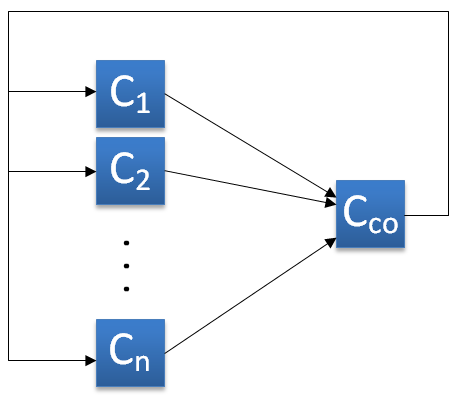
\includegraphics[width=\textwidth]{Figs/c_co.png}
		\caption{Components communicating via a central organising mechanism.}
		\label{fig:centralOrganizer}
	\end{subfigure}
	\begin{subfigure}[t]{0.45\textwidth}
		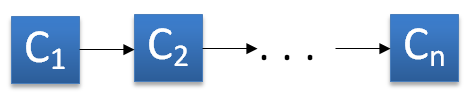
\includegraphics[width=\textwidth]{Figs/c_sequence.png}
		\caption{A sequence of components.}
		\label{fig:c_sequence}
	\end{subfigure}
\end{figure}

	
	\chapter{Affective Architecture}\label{ch:affectiveArchitecture}
	
	\section{Important Subsystems}\label{sec:someImportantSubsystems}

The global architecture now specified, we will introduce three related subsystems and fit them into this global framework: sensory perception --- the processing of raw sensory input into an format intelligible to other brain components ---, belief generation --- the imagination, which mimics the output of the senses ---, and affect --- broadly speaking, the emotional component of cognition.

\subsection{Sensory Perception}\label{sec:sensoryPerception}

The model presented herein is inspired by Marvin Minsky's ``The Emotion Machine''. Therein, Minsky proposes a layered mental structure where each successive layer operates on more and more abstract representations of the world, starting with primitive sensations and proceeding all the way to self-conscious reflection and rational planning. Figure~\ref{fig:brainLayers} shows such a layered structure.

 \begin{figure}[!h]
 	\centering
 	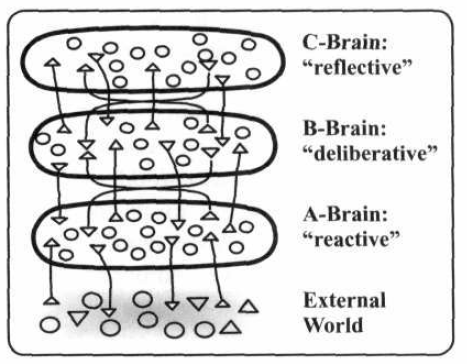
\includegraphics[width=300pt]{Figs/emotionMachine_brainLayers.png}
 	\caption{Layered perception of the world, from \cite[p.\ 100]{emotionMachine}.}
 	\label{fig:brainLayers}
 \end{figure}
 
 \newpage
 
The diagram is explained thus \cite[p.\ 100]{emotionMachine}:

\begin{quote}
	Now suppose that your A-Brain gets some signals from the external world (via such organs as eyes, ears, nose, and skin) --- and that it also can react to these by sending signals that make your muscles move. By itself, the A-Brain is a separate animal that only reacts to external events but has no sense of what they might mean. For example, when the fingertips of two lovers come into intimate physical contact, {\em the resulting sensations, by themselves, have no particular implications}. For there is no significance in those signals themselves: their meanings to those lovers {\em lie in how they represent and process them in the higher levels of their minds.}
\end{quote}

If we apply this to the architecture of Section~\ref{fig:global}, we can devise a system in which each sense $S$ has an associated component $C_S$ which does two things:
\begin{enumerate}
	\item Consume the raw sensory information delivered by various organs and output processed input for higher brain functions;
	\item as a side a effect of this processing, cause  instinctive, low-level reactions in the body, such as pulling away from pain or jumping at a sudden fright.
\end{enumerate}

In Figure~\ref{fig:sensoryPerception}, a slice of just such a system is shown for visual, auditory, olfactory/gustatory and tactile sensation. The produced data can be of two kinds: one is more abstract than the input and facilitates deliberative action, and the other contains instructions for instinctive behaviour for the body.

\begin{figure}[!h]
	\centering
	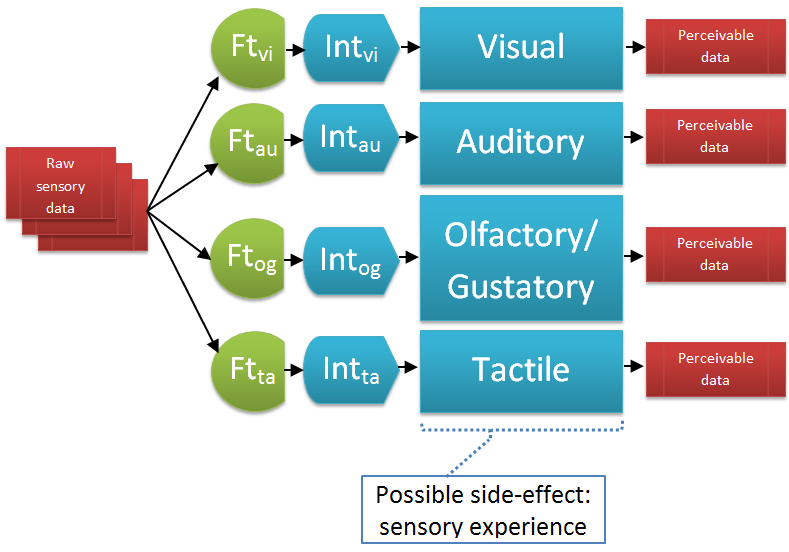
\includegraphics[width=325pt]{Figs/sensoryPerception.png}
	\caption{Partial structure of sensory perception - raw sensory data is processed and made available to higher functions such as the affective subsystem. The comment ``Possible side-effect: sensory experience'' signifies the fact that conscious and subconscious sensory experiences might occur as a side-effect of this processing. However, it is currently unknown to neuroscience whether this is indeed the case.}
	\label{fig:sensoryPerception}
\end{figure}


\subsection{Belief Generation and Planning}\label{sec:worldSimulation}

Broadly speaking, belief generation can be described as ``imagination'', and is closely related to sensory perception and world simulation. In examining the system, we might broadly classify its processes into three categories:

\begin{enumerate}
	\item Belief generation --- imagining sights, sounds, etc. Such experiences have much in common with those caused by our sensory organs, yet are marked not as real. In particular, imagined experiences evoke only parts of the conscious experience that accompanies real perceptions. Research by Berthoz and Lotze et al.\ suggests that (a) the brain indeed uses similar circuitry for real and imagined experiences and that (b) imagined experiences are prevented from being confused with real ones via inhibitory signals. Lotze et al.\ write \cite{lotze1999}:
	\begin{quote}
		The results of cortical activity support the hypothesis that motor imagery and motor performance possess similar neural substrates. The differential activation in the cerebellum during EM and IM is in accordance with the assumption that the posterior cerebellum is involved in the inhibition of movement execution during imagination.
	\end{quote}
	
	From the abstract of Berthoz's paper \cite{8713551}:
	
	\begin{quotation}
		\ellipses experimental evidence suggesting that the brain can use the same mechanisms for the imagination and the execution of movement. In particular the fact that adaptation of the vestibulo-ocular reflex can be obtained by pure mental effort and not solely by conflicting visual and vestibular cues has been suggestive of the fact that the brain could internally simulate conflicts and use the same adaptive mechanisms used when actual sensory cues were in conflict.
	\end{quotation}
	
	\item World simulation --- the imagination of future states. Simulating worlds goes beyond the imagination of sensory experiences; it involves constructing models of worlds and simulating their behaviour. The details of this process are unknown, but we can assert that it is capable of a number of things:
	\begin{enumerate}
		\item construction of non-physical worlds, such as mathematical models,
		\item extrapolation into the future and the past
		\item simulation of the minds itself and other agents.
	\end{enumerate}
	
	
	\item Executive planning --- humans can plan both both in immediate and concrete terms (such as body movement) and in the abstract. It is likely that different circuitry is used for movement planning and for planning involving abstract reasoning, in both cases it is necessary that the brain simulate the world in some way. The simulation of the consequences of body movement is likely older than humanity and distinct from the kind of world simulation described above, but both share their function: the agent proposes as series of actions to take, inserts them into some mental world and judges the utility of those actions based on the predicted consequences.
\end{enumerate}

Needless to say, that this process in all its subtleties is immensely complex and thus we simply endeavour to sketch its possible structure only in extremely rough outlines. This sketch is shown in Figures~\ref{fig:imagination},  \ref{fig:planner}, and \ref{fig:worldSimulatorPlannerInteraction}: the world simulation is an ordinary component with a filter and interpreter which outputs, for simplicity's sake, messages marked as imaginary. We can imagine such messages to be very much like ordinary sensory ones, with the exceptions that they have no accompanying sensation and, more importantly, that we are aware of their non-reality. The planning component receives instructions about desirable states and outputs hypothetical actions which the world simulator incorporates. The world simulator's output is in turn read by the planner, which then abandons the plan or decides to pursue it further.

\begin{figure}
	\centering
	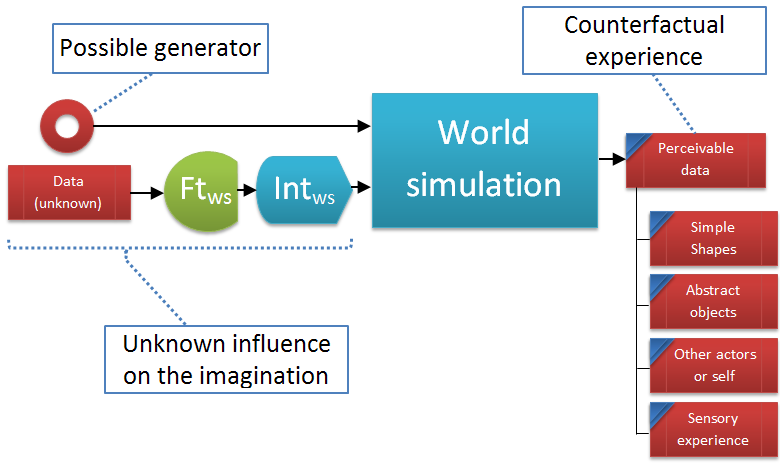
\includegraphics[width=\textwidth]{Figs/imagination.png}
	\caption{Structure of of belief generation \& world simulation: messages emulating the output of sensory perception are generated, but are marked as imaginary by unknown means.}
	\label{fig:imagination}
\end{figure}

\begin{figure}
	\centering
	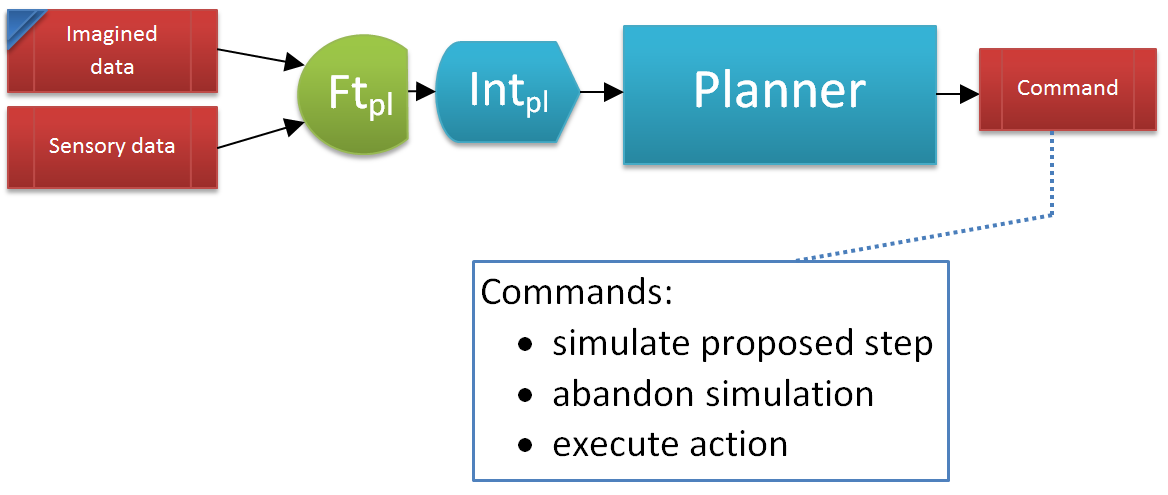
\includegraphics[width=\textwidth]{Figs/planner.png}
	\caption{Planner with two kinds of inputs: (1) real sensory data and (2) imaginary data which comes from world simulation. On the basis of these inputs, possible steps are developed and sent out as commands.}
	\label{fig:planner}
\end{figure}

The planner, minimally, has to perform two functions --- first, it has to judge the desirability of various world states and second, it has to be able to devise possible steps for the agent based on some strategy. If these two functions and some desired goal(s) are given, the planner can do its work by issuing the following commands, as shown in Figure~\ref{fig:planner}:
\begin{enumerate}
	\item If some goals are not yet reached but appear possible, devise possible steps to take and have the world simulator predict their outcomes.
	\item If the goals appear impossible the necessary steps prohibitively undesirable, command the world simulator to cease its activity.
	\item If earlier proposed steps turn out to fulfil some goal, contact the agent's executive component.
\end{enumerate}

\begin{figure}
	\centering
	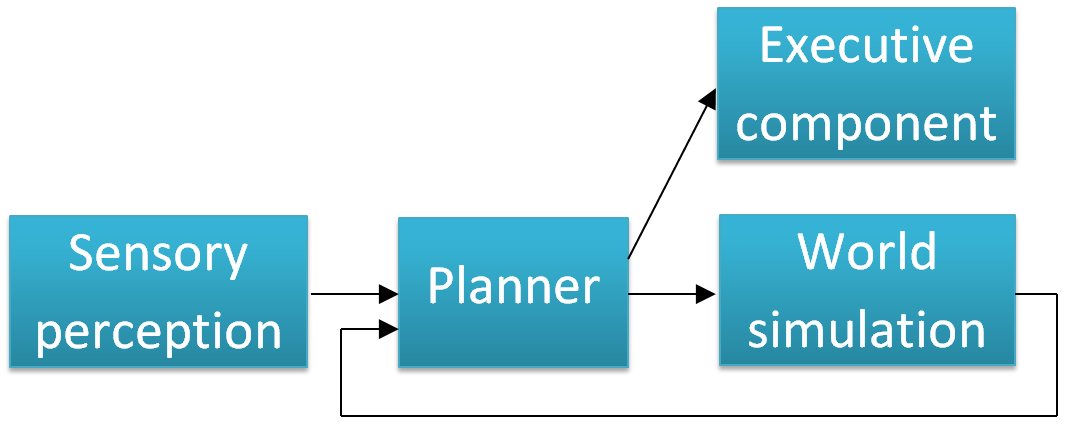
\includegraphics[width=\textwidth]{Figs/worldSimulatorPlannerInteraction.png}
	\caption{Interaction between world simulator and planner: the planner devises possible steps and feeds them into the world simulator, which, in turn, tries to calculate their effects. The results are fed back to the planner.}
	\label{fig:worldSimulatorPlannerInteraction}
\end{figure}

\subsubsection{World Simulation as Rationality}
The way in which we just described the interaction between the world simulator and the planner suggests that they function as a pair of guesser and checker: the planner generates ideas on what to do and the world simulation tests their viability in some setting. Indeed, we can model rational thinking as embedded in the world simulator, especially if we make use of a plastic neural system. The proposed steps of the planner might be quite chaotic and irrational, but when given to the world simulator, it recognises them as such and returns a failure signal to the planner, causing it to abandon ``bad'' paths of cognition. A plastic planner can learn from the consistent failure of certain kinds of steps and, in time, propose them less and less often. Observed as a whole, this system of planner and simulator appears to simply deliver good plans by intuition, even though, in isolation, neither part is very clever.\footnote{We do not wish to idealize rationality too much; world simulation is only partly rational and, given faulty information about the world, will err considerably and in documented ways. Similarly, it is certainly possible for the planner to derange the world simulator by evaluating certain states as so desirable/undesirable that it will pursue even scenarios which the world simulator reports as highly unlikely.}

\paragraph{Model.} In a simplified way, we can model the process of logical deduction in a formal system $F = (A, R)$, where $A$ is a recursive set of axioms and $R$ is a recursive set of production rules of the form $(r_{\mt{from}}, r_{\mt{to}})$ s.t. $r_{\mt{from}} \rightarrow r_{\mt{to}}$ is a valid production in the system. Let
	\begin{enumerate}
		\item $W$ be a world simulator for the world of propositions $\mathcal{P}$ in $(A,R)$,
		\item $P$ a planner,
		\item $\mathrm{St} = \{s_1,\dots,s_p\}$ a set of messages about steps to take,
		\item $\mathrm{Cat} = \{K_1,\dots,K_q\}$ a list of message categories,
		\item $\field{cur} : W_S$ the current state of the world simulator,
		\item $\field{ins} :: W_S \rightarrow \mathrm{St} \rightarrow W \rightarrow W$, $\field{del} :: \mathrm{St} \rightarrow W \rightarrow W$ functions for inserting or deleting a state change into the world simulator or the planner,
		\item $t(i)$ and $b(i)$ functions which increase or decrease the likelihood of sending a message belonging to category $K_i$ and 
		\item $\bot_{i}, \top_{i}$ the failure and success signals of a message belonging to the category $K_i$.
	\end{enumerate}
	
One step of the interaction between $W$ and $P$, in a scenario where $P$ proposes steps $s_{i_1},\dots,s_{i_n}$, can then be modelled with two traces $T_{\mt{guess}}$ and $T_{\mt{check}}$:

$$
	\begin{array}{l l l}
		T_{\mt{guess}}(\tt{step}) & \equiv & \sendsf{P}{\tt{ins cur step})}{\tt{step}}{\tt{step}}{\tt{ins cur step})}{W}\\
		\\
		T_{\mt{check}}(\tt{step}) & \equiv &
		\forall K_i \in Cat: K_i(\tt{step}) \Rightarrow\\
		
		& & \hspace{1cm} \mt{if } \exQ{s_j} (\field{cur}, s_j) \in R\ \mt{ then } \
					\sendsf{W}{}{\top_i}{\top_i}{t\ i}{P}\\
		& & \hspace{1cm} \mt{else }\ \sendsf{W}{\tt{del step})}{\bot_i}{\bot_i}{\tt{del step}, b\ i}{P}\\
	\end{array}
$$

\medskip

Axioms can be selected by executing $T_{\mt{guess}}(\tt{ax})$ for all $\tt{ax} \in A$. We can then perform deduction via $T_{\mt{guess}};T_{\mt{check}}$, for a probabilistically selected $\tt{step} \in St$.

Intuitively, $T_{\mt{guess}}$ guesses a step to take. It does so but inserting it into the planner's world-state via $\tt{ins}$ and then sending a message to the world simulator, which also inserts it into its world state. $T_{\mt{check}}$ then checks whether the change from $\tt{cur}$ to $\tt{step}$ was legitimate. If so, it determines to which category $\tt{step}$ belongs and sends the $\top$-signal for that category back to the planner. Otherwise, it sends the corresponding $\bot$-signal. The purpose of this is to make it more or less likely, respectively, that the planner should choose the same category of step in the future. The categories, we can imagine, could be things like ``modus ponens'', ``associative reasoning'', ``appeal to consequences'' and so forth.

If we repeat this interaction (with different proposed steps $s_1,\dots,s_p$ in each iteration), we get an algorithm for logical deduction  --- that is, since $A$ and $R$ are recursive, the system will recursively enumerate all valid logical formulas, provided that we pursue each path and that the probability of selecting any valid step is $> 0$. In addition, we could add a goal function $g$ to $P$ s.t. it would accept certain states and stop. Thereby, $P$ and $W$ could be used to prove logical propositions.

\subsection{Affect}\label{sec:affect}

When discussing human affect, one can mean various things: the causation of emotion, its internal mechanisms, the expression of emotion, social communication of emotions, etc. In this document, we restrict our attention just to the internal mechanisms --- that is, to the means by which emotions are evoked in an agent and how they shape its thinking.

Furthermore, the issue will only be the causative mechanism itself; taxonomy and hierarchy of emotions are deferred to future versions of this document.

The model presented herein is adapted from Gadanho and Hallam \cite{DBLP:journals/adb/GadanhoH01}, who employed it in the context of robot learning. They constructed a system of \emph{feelings} and \emph{sensations} $\mathcal{F}$, \emph{emotions} $\mathcal{E}$, and a hormone storage $H$.

\begin{figure}[!h]
	\centering
	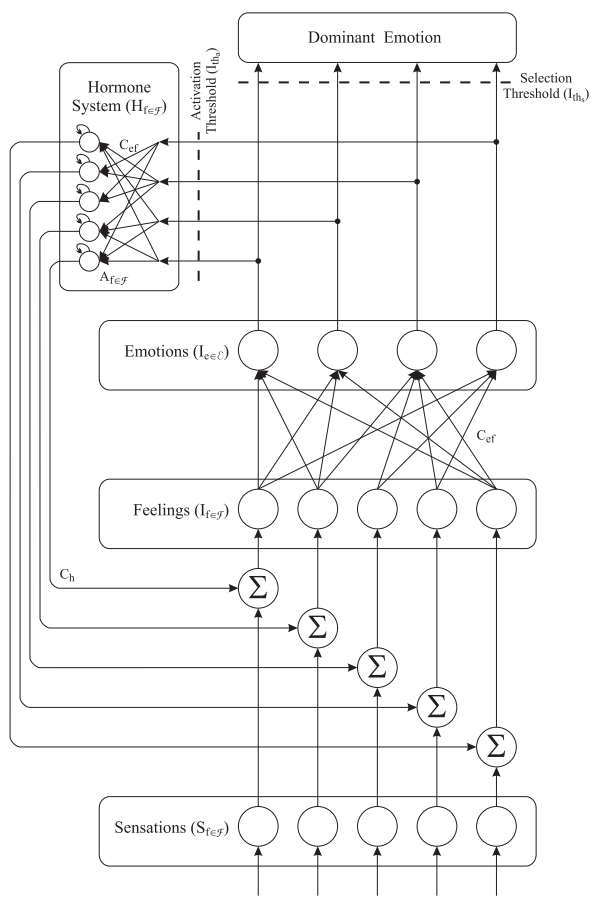
\includegraphics[width=200pt]{Figs/gadanhoModel.png}
	\caption{Emotional model of Gadanho and Hallam \cite[p.\ 46]{DBLP:journals/adb/GadanhoH01}.}
	\label{fig:gadanhoModel}
\end{figure}

Figure~\ref{fig:gadanhoModel} shows this model: \emph{sensations} enter the system and are connected to the \emph{feelings}. They, in turn, determine the agent's \emph{emotions}. The emotions then feed into a \emph{hormone storage}, the contents of which influence, together with the \emph{sensations}, the agent's \emph{feelings}. In the context of their paper, this model had a very restricted application. Its purpose was to merely help guide a robot through a world, and accordingly, $\mathcal{F}$ and $\mathcal{E}$ were only defined as \cite[p.\ 47]{DBLP:journals/adb/GadanhoH01}:
$$
	\begin{array}{l}
		\mathcal{F} = \{ \mt{Hunger}, \mt{Pain}, \mt{Restlessness},
						 \mt{Temperature}, \mt{Eating}, \mt{Smell},
						 \mt{Eating}, \mt{Proximity} \}\\
		\mathcal{E} = \{ \mt{Happiness}, \mt{Sadness}, \mt{Fear},
						 \mt{Anger} \}
	\end{array}
$$

\begin{figure}[!h]
	\centering
	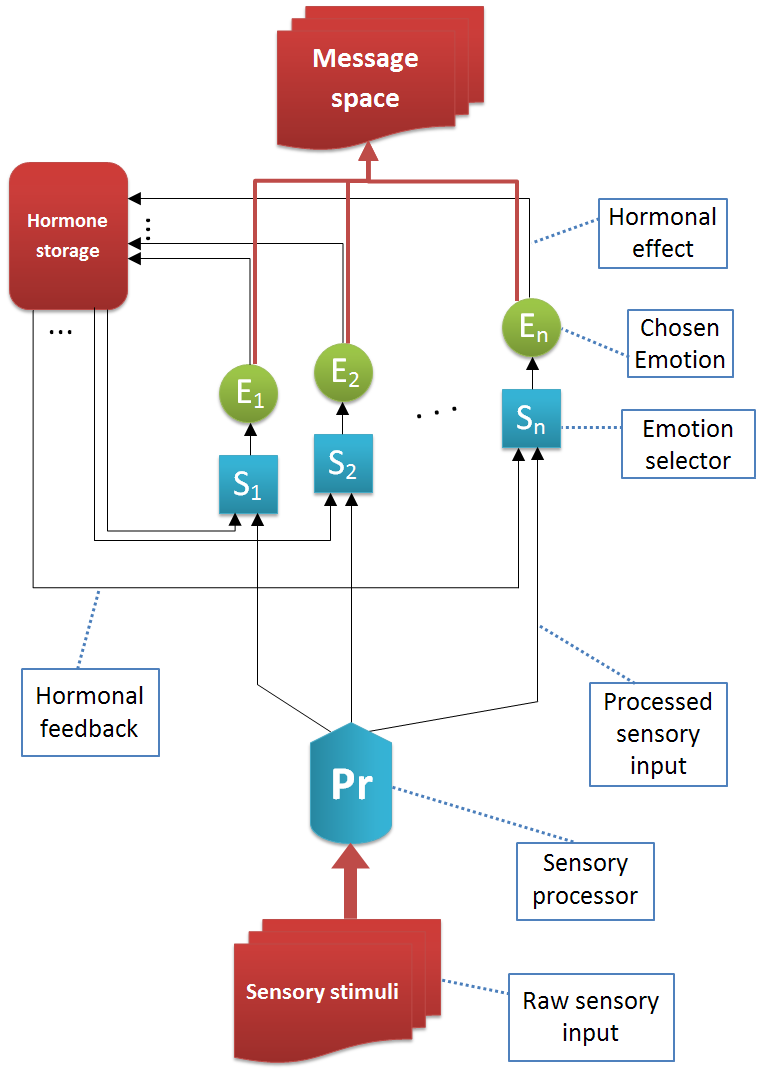
\includegraphics[width=400pt]{Figs/affectiveSubsystem.png}
	\caption{Affective subsystem; specialisation of the global neural architecture. In plastic neural systems, selections may change over time.}
	\label{fig:affectiveSubsystem}
\end{figure}

\pagebreak
The main advantage of Gadanho's and Hallam's model is that (a) it is sufficiently generic to accommodate various schemas and (b) posits an internal state (the hormone storage), giving agents a certain inertia. For example, one can imagine integrating a many-dimensional model like Brazeal's \cite{breazeal2003} detailed taxonomy of emotion like Ortony's OCC model \cite{ortony1988}. The existence of an internal state is necessitated by the simple observation that our internal world is not solely dependent on momentary stimuli, but merely influenced by them. The idea of a hormone storage might be a simplistic approximation but it, too, can be refined as needed.\footnote{It might be tempting to simply replace the hormone storage with the message space, but doing so would ignore the role that neurotransmitters like dopamine and serotonin play in cognition, irrespective of the purely computational activity of brain components.} Figure~\ref{fig:sensoryPerception} shows the adapted model. The general structure was retained, but the set of sensations was replaced by the sensory processor described in Section~\ref{sec:sensoryPerception} and, instead of a single dominant emotion, competing emotions simply emit messages which are used by execute components and the world simulation.

\subsubsection{Affective Subsystems}

In this section, We will develop the concept of ``emotion'' in greater detail. The process shown in Figure~\ref{fig:affectiveSubsystem} might suggest we simply have a collection of emotions and that all emotions are essentially equal, but we submit that this is not so. Instead, we propose the existence of various subsystems, each responsible for a group of emotions, and each with its own history and distinctive tasks. In the rest of this work, the following two assumptions will be made:

\begin{enumerate}
	\item {\em ``Emotion'' is not a singular phenomenon.} Specifically, this is contradicts many-dimensional models of emotions which propose one, two, three or four axes and a corresponding vector space in which every emotion is a point. Such a view implies that all emotions share a neurological template which is parametrized with coordinates to result in different experiences.
	\item {\em There exist emotions which are both different in kind and which pertain to different subsystems in the brain.} This implies that emotions cannot morally be seen as a homogeneous set $\{E_1,\dots,E_n\}$. Instead, a number of distinct subsystems are necessitated, each responsible for the causation and processing of a group of emotions. Given this, the only substantial aspect any two emotions might have in common would be our referring to both of them as ``emotion''.
\end{enumerate}

Both of these assumptions are rather concrete and thus deserve evidence. In 1999, Davidson and Irwin, using PET and fMRI scanning, found two different systems mediating approach- and avoidance related behaviours \cite[p.\ 13]{davidson1999}:

\begin{quote}
A large body of lesion, neuroimaging and electrophysiological data supports the view that the prefrontal cortex (PFC) is an important part of the circuitry that implements both positive and negative affect. ($\dots$)
A number of early studies that evaluated mood subsequent to brain damage suggested that patients with damage to the left hemisphere, particularly in PFC, were more likely to develop depressive symptoms compared with patients having lesions in homologous regions of the right hemisphere. ($\dots$)
The general finding of left dorso-lateral PFC damage increasing the likelihood of depressive symptoms has been interpreted to reflect the contribution of this cortical territory to certain features of positive affect, which, when disrupted, increases the probability of depressive symptomatology.
\end{quote}

In this, they echo earlies findings by Cacioppo et al.\ \cite{cacioppo1999}, Gray \cite{gray1994} and Lang et al.\ \cite{lang1990} that affect is lateralised, with different hemispheres being responsible for different categories of feeling. It therefore stands to reason that different emotions, being generated by different brain regions, should therefore also be different in their character.

Further, much research has been done in the area of so-called {\em basic emotions} --- a small set of emotions are acknowledged as being both elementary and characteristically distinct from each other. The Cambridge Handbook of Affective Neuroscience provides a good overview of the basic emotion theory \cite[pp.\ 9-10]{cambridgeAff}. Matsumoto and Eckman \cite{matsumoto2009}, for instance, identified seven basic emotions: happiness, surprise, contempt, sadness, fear, disgust, and anger.

Damasio \cite{damasio1998}, drawing upon neuroscientific findings, sketches a model of affect mainly involving the prefrontal cortex, but also the amygdala, the hypothalamus, and the anterior cingulate cortex, as seen in Figure~\ref{fig:damasioSystem}.

\begin{figure}
	\centering
	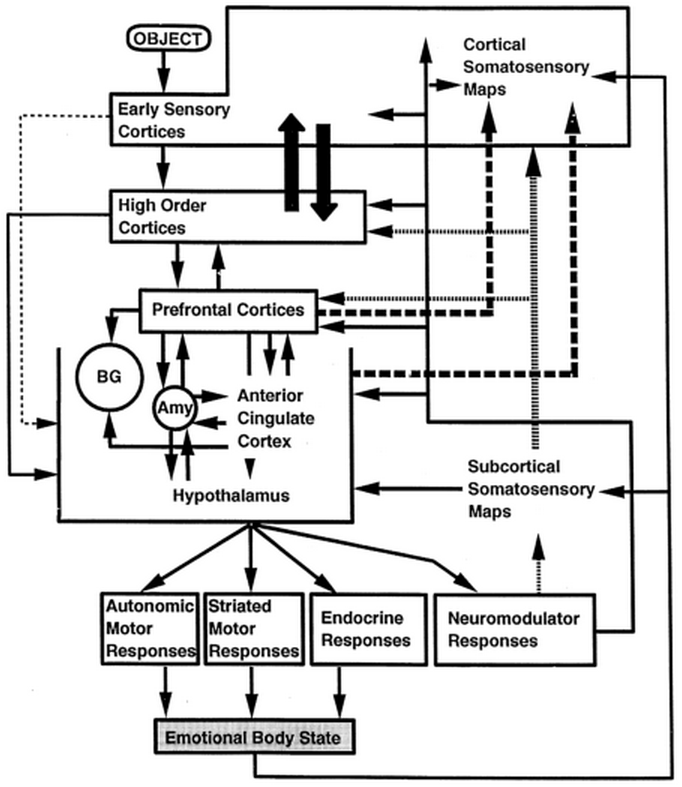
\includegraphics[width=250pt]{Figs/damasioSystem.png}
	\caption{Neurological structure of affect, according to Damasio \cite{damasio1998}.}
	\label{fig:damasioSystem}
\end{figure}

In the same article, he describes how different brain regions are responsible for different kinds of emotion:

\begin{quotation}
	Equally problematic is the widespread view that the limbic system is the neural basis for all emotions. A rich body of evidence tells us that this is just not the case. Both within and around the limbic system, circuitry connection varied neural sites supports the operation of different emotion. For instance, work on aversive conditioning in rodents has shown that the amygdala is certainly involved in negative emotions such as fear [10,6]. {\em Work in humans, on the other hand, has not only confirmed the amygdala's involvement in negative emotions such as fear and anger, but also shown that the amygdala is not involved in the processing of positive emotions such as happiness, or negative emotions such as disgust.} [emphasis mine]
\end{quotation}

The last sentence of that quotation is especially revealing: it states that the neurological distinction is not simply one between positive and negative, or one between approach- or avoidance-related emotions, but that each emotion has its own profile of neurological activity and involves its own peculiar set of brain structures.

These facts make it quite clear that emotions are not simply homogeneous phenomena, being induced by a single system in the brain; rather, they are different in character and in the neural structures they involve. 

\paragraph{Structure of affect.} The system depicted in Figure~\ref{fig:affectiveSubsystem} left several parts unspecified: the sensory processor $\Pr$, the emotion selectors $S_1,\dots,S_n$ and the messages sent by the chosen emotions into the message space. In the following paragraphs, we will flesh out that model in greater detail, building principally on the work of Sander, Grandjean and Scherer \cite{DBLP:journals/nn/SanderGS05}. Sander and colleagues partitioned the emotion process into four stages, as shown in Figure~\ref{fig:sanderSystem}. The first is {\em relevance}, which functions as a filter and detects the intrinsic pleasantness and the level of (emotional) attention that a stimulus demands. The processes of this stage, roughly speaking, correspond to the work of the sensory processor $\Pr$. The second stage is {\em implication}, where reasoning becomes engaged in order to determine the cause, likely outcome, and urgency of the perceived facts. At this stage, emotions like joy, anger, contentment, disgust, etc. are evoked, together with approach- and avoidance-related behaviours --- this corresponds to the emotion selectors $S_1,\dots,S_n$. Deliberate strategies come only in the next stage: {\em coping}. In it, reasoning and planning become fully engaged. The fourth stage is {\em normative significance} and deals, in essence, with moral concerns, both internal and those of other agents.

\begin{figure}
	\centering
	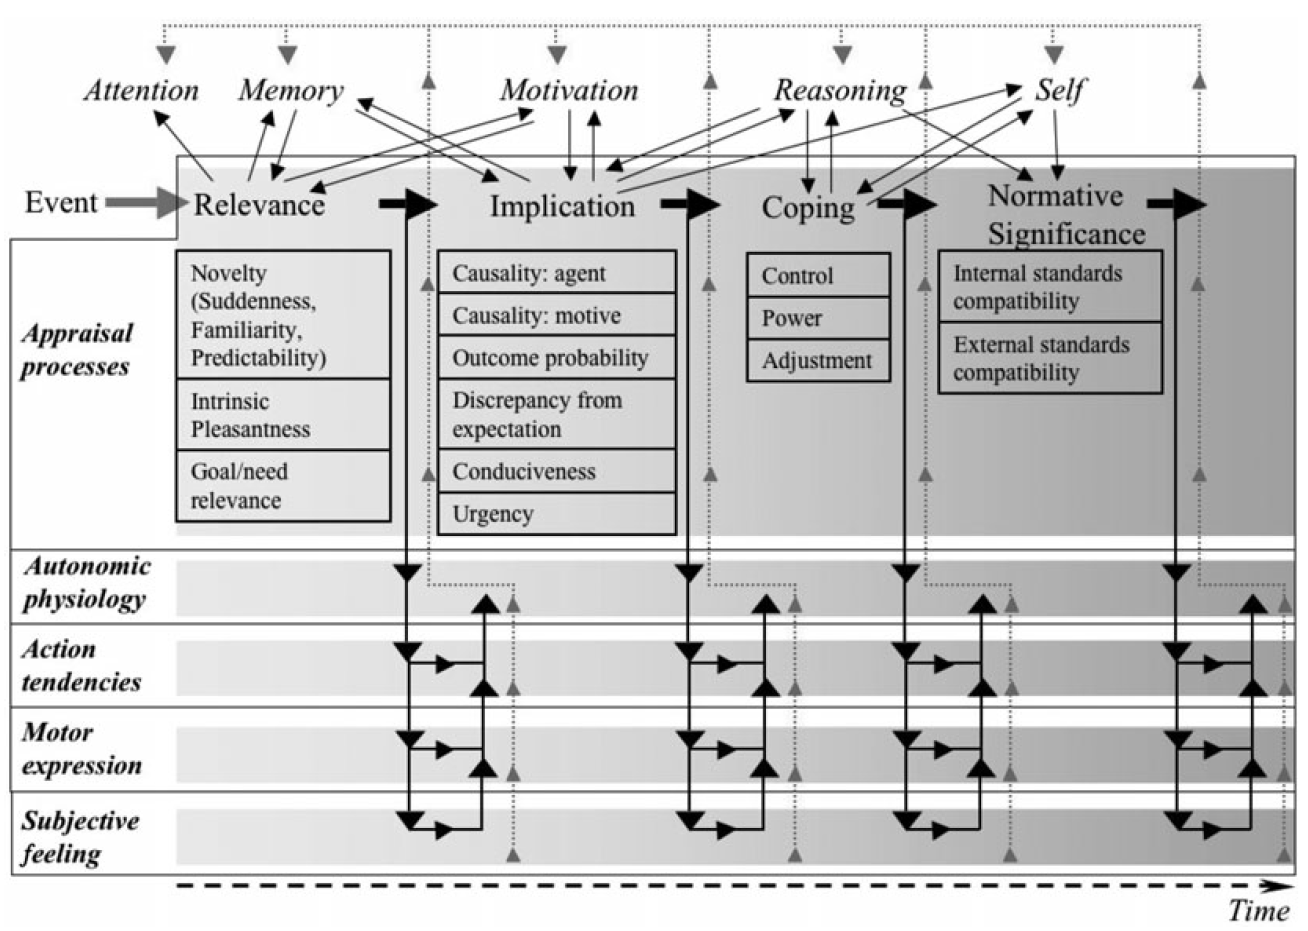
\includegraphics[width=440pt]{Figs/sanderSystem.png}
	\caption{The four-stage emotion process according to Sander et al, consisting of relevance, implication, coping and normative significance.}
	\label{fig:sanderSystem}
\end{figure}

Sander et al.\ give a good, detailed account of the interactions of affect with other systems, although we would argue that theirs is unduly suggestive of a simple {\em pipeline}, rather than a mesh of systems into which the affective ones are embedded. In addition, it does not address the interactions with perception, memory, and reasoning. Based on the evidence discussed above, we shall now present a more horizontal view and construct a model of the hypothesized emotional subsystems and their interactions with other parts of the brain. Since no established vocabulary seems to exist in this specific are we shall first introduce a number of terms.

\begin{definition}[Evocative system]
An evocative system is a subsystem in the brain responsible for evoking consciously experienced affect within an agent based on internal or external stimuli.
\end{definition} 

Various such evocative systems can be imagined. For the purposes of this thesis, we will work with the following rough categorization:

\begin{description}
	\item[Pre-social emotions.] Certain behavioural mechanisms can be observed in non-social as well as social animals. The fight-or-flight instinct, for example, is nearly universal, as is the inclination to seek out food, shelter, and other resources. ``Instinct'' is indeed a more appropriate term in the case of most species, rather than ``emotion'', which connotes a certain richness of experience. Nonetheless, we can clearly see that, in more intelligent, social animals, emotions like anger, fear, and joy, have grown out of just these instincts. Hence the term ``pre-social emotions'': while emotion itself is quite possibly inherently social, certain emotions are rooted in instincts which are not, and an emotional animal would feel them even if it were the only one of its kind in an environment.
	
	\item[Social emotions.] A by far richer subset of emotions are the social ones. Indeed, social situations are the ones where affect can and must truly shine: the presence of other individuals, or of the entire tribe, demand a variety of affect relating to the appraisal of the agents, sympathy/antipathy, respect/contempt, the appraisal of oneself, showing dominance or submission, influencing other group members, taking action as a group, judging the behaviour of agents against norms, etc. It is also in social emotions in which it even makes sense to {\em show} emotion: facial expressions and gestures provide the signalling and mechanism needed for group coherence and coordinated action.
	
	We can identify several subsystems in the category of social emotion:
	
	\begin{enumerate}
		\item Reflective judgement about oneself in relation to the group or to abstract norms, primarily pride and shame \cite{Teroni2008}, but possibly also jealousy and humiliation (which, in contrast to shame, is attributed to external causes) \cite{fontaine2009};
		\item other-related judgement which determines whether to feel sympathy or antipathy, compassion, respect or contempt, trust or distrust for other individuals;
		\item normative judgement, which determines whether others or oneself is acting in accordance with instinctive or cultural norms.
	\end{enumerate}
	
	Other classifications are also possible. Haidt \cite{haidt2003}, for example, identifies those that are other-condemning (disgust, contempt), self-conscious (shame, embarrassment), other-suffering (compassion), other-praising (gratitude, awe). The picture is immensely complex and the neurological structure is presently not known. For the purposes of this thesis, we will therefore content ourselves with only this roughest of outlines.
	
	\item[Aesthetic emotions.] This type of emotion is perhaps the least studied in neuroscience and AI. It is certainly the most subtle and the least ``utilitarian'' type --- as such, it is philosophers, rather than AI researchers, who study it. For instance, Jenefer Robinson, in {\em Deeper Than Reason: Emotion and Its Role in Literature, Music, and Art} \cite{robinson2005}, writes about the affective appraisal of artwork as an unconscious process which partly reproduces the emotions of its creator. In this, she builds upon and modifies Collingwood's 1983 {\em The Principles of Art} \cite{collingwood1938, SEPcollingwood}. Since aesthetics are not the focus of this work, we shall leave it at this mention. A more thorough exploration would be interesting future work, however.
\end{description}

The emotions just listed can all be found in the more extensive taxonomies, chiefly among them in Ortony's OCC model \cite{ortony1988}. The taxonomies, however, tend to neglect the underlying neurology and the chronology of the development of these systems. Ortony's classification specifically is persuasive up to a point, but, despite it being fine-grained, one is left wondering about the underlying structure: which emotions are caused by the same brain regions, what structure, if any, do two given emotions share, to what degree is the classification scheme isomorphic to the actual neurology? This is an active area of research and while these questions are interesting, we have to leave them largely open for now.

The evoked feelings tie into and directly influence the agent's actions. This includes conscious, deliberate ones, such as avoiding an unsympathetic person, but also subconscious ones and those that are purely internal, such as the focusing one's attention to an important topic. These actions all fall under the umbrella term of {\em executive system}:

\begin{definition}[Executive system]
An executive system is a subsystem in the brain which makes decisions about the behaviour of an agent's mind or muscular system.
\end{definition}

This definition leaves open what exactly a decision is. In principle, any neural activity in a part of the brain could be seen as a decision of sorts, since it influences neural activity in other parts. While we do perceive certain processes as deliberate and others as automatic, this is simply what our introspection tells us and does not reflect the underlying reality; (conscious) decision-making is as mechanical as any other process in the brain, the chief difference being that we are aware of the workings of that process and perceive the control it exerts over cognition as coming from us.\footnote{We should add that we are not even aware of the entirety of our decision-making. This is especially apparent when we are asked to make trivial or random choices. A person who is asked to press a left or a right button, for example, will choose one, seemingly at random, but will not be able to explain why one button was chosen over another. Moreover, there is evidence that the choice is made before the person {\em knows} that a choice was made: Soon et al. \cite{soon2008} instructed subjects to press a button and to record when they thought they made the decision to do so. Brain scanning revealed spikes in the activity of the lateral and medial frontopolar cortices and the posterior cingulate cortex {\em before} the subjects claimed their decisions were made. In effect, they only became aware of their supposedly free decisions after they had already been made. From their conscious perspective, the decision simply ``popped into their heads''.}

Nonetheless, there are properties by which we can identify executive systems in the brain: on a sufficiently high level of abstraction, we can see that certain components are receptive to control signals. Certain other components --- these are the executive systems --- have as their {\em chief purpose} the sending of such control signals. The former accomplish some conceptually small task and essentially serve as building blocks. The latter structure the work and assemble the small building blocks into compound actions. See Section~\ref{sec:worldSimulation}, where planner and world simulator work in tandem, with the world simulator bearing the workload and the planner having control.

We can now distinguish certain kinds of action. While those performed with the ``body'' (i.e.\ the skeletomuscular system) are the most visible ones, we, as shown, also make decisions regarding the contents of our minds --- we decide {\em what to think about}. We then add the distinction between consciously and subconsciously made actions and get the following four categories of executive system:

\begin{description}
	\item[Subconscious motor control:] instinctive reaction, such as the jerking away from pain, jumping when startled, and turning towards interesting visual stimuli.
	\item[Conscious motor control:] deliberate, planned action which the agent experiences as a choice.
	\item[Subconscious mental control:] involuntary but consciously experienced changes to the mind-state of an agent which are perceived as activity rather than mere feeling. This includes like obsessing over an issue, manias, fantasies insofar as involuntary, etc.
	\item[Conscious mental control:] deliberate mental changes of an agent. This includes the making of decisions, the deliberate focusing of attention, deliberate planning, deliberate strategy selection, and so forth.
\end{description}

We stress that these are {\em categories} of systems, not systems themselves. We control our minds and our bodies in a variety of ways and there is no evidence that there is some sort of master control system anywhere in the brain responsible for these tasks. The planner from Section~\ref{sec:worldSimulation} only controls one other component --- and it might very well be that it does not even exist in the brain as one compact component. It might be that a variety of smaller systems are tugging and vying for control and balanced against each other in such a way that the illusion of dedicated planning component is created.

\section{Interaction Between Affect and World Simulation}\label{sec:interactionBetween}

Section~\ref{sec:worldSimulation} outlined what could be called {\em deliberate action} in the from of a planner-world-simulator loop. Section~\ref{sec:affect} described the structure and components of affect. These systems are of course not isolated from each other; emotional states influence both the planner's chosen heuristics and the world simulator's creation of worlds. In addition, attention, also influenced by affect, controls the allocation of cognitive resources. We now explore these relationships in further detail.

\paragraph{Planning as search.} In the AI literature, search algorithms are of great importance. In this context, we can view the loop between planner and world simulator as a greedy search: the planner chooses the nodes which are to be expanded and sends them to the world simulator. It, in turn, performs the expansion by simulating the appropriate worlds. These simulated worlds are sent back to the planner for evaluation regarding desirability (i.e.\ cost). This presents an obvious problem: since greedy search is not complete, our planner-world-simulator loop can't be complete either. In fact, the situation is worse --- greedy search computes the cost of all candidates for expansion and chooses the cheapest, whereas our planner, being heuristic, might not consider certain nodes at all.

This might seem damning, but we must also consider the interaction with attention and memory. First, planned steps are committed to memory and thus, we gain access to past costs. An agent does not plan blindly, but can recall how long its plans are and what costs past planned steps entail. Given this information, we can turn the greedy algorithm into an A$^*$ search, with the qualification that the planner might not consider certain nodes. The mechanism of attention can further be used to enhance the search: if planning along a certain path takes too long, the agent might decide to abandon it altogether and start afresh with a different strategy. This failure too is stored in memory and can influence the planner in the new planning process by making the proposing of steps of the previously pursued path  unlikely.
	
	\chapter{Implementation}\label{ch:implementation}
	
	Having laid the theoretical framework, we come to the practical part of this thesis --- a proof-of-concept implementation of multiple affective agents interacting with each other. This section contains the following parts: (1) the world in which act, (2) the architecture of these agents, and (3) the evolutionary changes in the agent pool from generation to generation.

The goal is the creation of toy AI that semi-realistically mimics animal intelligence, the operative word being "mimic". As Sloman \cite{sloman2000} pointed out, naming a variable \textsc{anger} or \textsc{love} does not give a program some qualitative experience. No; our much more modest goal is to \textsc{emulate} the behaviours that are associated with certain mental states --- and to show how such emotional states, interacting with reasoning, can help an agent thrive in its environment. These programs will really only be soulless automata, employed to illustrate a point about living beings with brains, acting with incomplete information.

\subsection{World}

The choice of the world profoundly affects the implementation of the agent --- its knowledge base, mechanism of perception and interaction, the required complexity of the implementation. On the one hand, the world should be simple enough to permit a reasonably small and effective agent which does not have to solve hard AI problems (like human-level sight) to deal with what we, in this context, might call details --- but on the other hand, the world should be sufficiently complex to allow agents to distinguish themselves. This is especially true in the case of an affective agent whose actions should be visibly influenced in rich and subtle ways by its emotional state. I shall first lay out the design goals and then evaluate three possible worlds for agents.

\paragraph{Design Goals.} The two most important criteria for prospective worlds are richness of interaction and world complexity, in that order. As said, an evaluation of affective agents is only possible if they can interact with their environment and other entities in a sufficiently complex way to allow agents with different emotional profiles to be distinguished from each other. Mechanisms of problem-solving like STRIPS \cite{fikesNilsson}, A* \cite{nilssonAStar}, ASP \cite{asp1}, forward-/backward-planning, etc. have been explored in the context of structurally simple worlds, generally those representable through propositional logic, cost-functions, decision tress, and the like. While these are useful, they are less appropriate in an affective scenario for the following two reasons:

\begin{enumerate}
	\item they are geared towards finding provably optimal solutions to computationally expensive but conceptually simple problems like planning or game-playing and
	\item they rely heavily on hand-crafted ontologies and domain knowledge on the part of the human programmer.
\end{enumerate}

For a world to be useful to us and to avoid these pitfalls, it should be in some sense realistic: it should permit a large number of different kinds of interactions, and it should not provide agents in it with perfect knowledge about its rules. 

I admit that I here stand in opposition with Marvin Minsky, who famously recommended the use of idealized micro-worlds to study artificial intelligence, in that same vein in which physics makes use of ideal, frictionless planes and perfect spheres. His argument certainly has merit, but I believe that emotion is too complex a phenomenon for such abstract scenarios. In too simple a setting, pure reasoning not only easily outperforms emotional behaviour, but avenues for exhibiting emotional behaviour are scarce to begin with. For this reason, I propose that, in this context, rich interactions should take precedence over idealization and simplicity.

It is of course still desirable to minimize complexity as far as possible. An overwhelmingly complex world has two obvious drawbacks: first, the required complexity of an agent scales with the complexity of the world; second, the more complex the world, the harder it is to reason about it. If there are a hundred ways to succeed, for instance, agent performance becomes quite difficult to measure.

\subsubsection{Block World}

Block worlds are the simplest type of abstract world, and many variations exist. They all have in common a number of shapes placed on top of each other in a 2-dimensional world. An agent can pick up and move a shape if and only if there are no other shapes on top of it (and if it is not already holding one). The goal generally consists of achieving some desired configuration of shapes, such as building or piecewise transporting a tower, or collecting all red triangles. 

Micro-worlds like blocks worlds have been extensively studied. In this, their simplicity has been their great advantage --- that very simplicity is a serious problem for us, however. Affect is inherently a subtle and social phenomenon; it is not clear how it could be believably exhibited in such an abstract and simple world. The very same properties which expedite their theoretical study make them useless for our evaluation.

%\subsubsection{Real world}

\subsubsection{Wumpus World}

The traditional Wumpus world, as described in Russell and Norvig's {\em Artificial Intelligence: A Modern Approach} \cite[p. 236]{norvig}, is a grid-based, 4x4 cave world with one agent, one monster --- the Wumpus --- and gold placed in random rooms. The agent starts at position $\langle 1,1\rangle$ and can move forward or turn 90$^\circ$ to the left or right. If it enters a room with a pit or a live Wumpus, it dies; its goal is to find and collect the gold and then move back to position $\langle 1,1\rangle$ to climb out of the cave. In addition, it has one arrow which he can fire straight ahead to defend against the Wumpus. The agent has only the following local information \cite[p. 237]{norvig}:
\begin{itemize}
	\item In the square containing the Wumpus and in the directly (not diagonally) adjacent squares, the agent will perceive a {\em Stench}.
	\item In the squares directly adjacent to a pit, the agent will perceive a {\em Breeze}.
	\item In the square where the gold is, the agent will perceive a {\em Glitter}.
	\item When an agent walks into a wall, it will perceive a {\em Bump}.
	\item When the Wumpus is killed, it emits a woeful {\em Scream} that can be perceived anywhere in the cave.
\end{itemize}

This type of world is simple enough to be amenable to rule-based reasoning, although it can contain ambiguous situations where the agent does not have enough information to make the best choice. For example, if an agent moves to position $\langle p_x,p_y \rangle$ and experiences a breeze, 1, 2, or 3 adjacent rooms may contain pits, but it cannot be safely determined which ones these are. Thus,  occasionally, the agent must choose between climbing out without the gold and risking death by pit or Wumpus.

For our purposes, this is a bit too simple, however. Caution/bravery is the only axis along which agents can be differentiated and although various complex behaviours --- such as trying one dangerous cell, then going back and trying another one to explore the world --- are possible, these do not have a clear relation to emotional states.

Let us, while staying true to the spirit of the original, now define a type of extended Wumpus world \wext\ that allows more varied interaction between agent an environment.

\begin{definition}[\wext-type world]\label{def:wext}
	Let $\type{T_v}$, $\type{T_e}$, $\type{T_g}$ be arbitrary types. Further, let $G$ be a directed graph with vertex labels of type $\type{T_v}$ and edge labels of type $\type{T_e}$, and let $\mathrm{gl}$ be an object of type $\type{T_g}$. Then the tuple \tuple{G, \mathrm{gl}} is a \wext-type world \paren{with type parameters $\type{T_v}$, $\type{T_e}$, $\type{T_g}$}. We call $G$ the {\em world frame} and $\mathrm{gl}$ the {\em world data}.
\end{definition}

We can interpret each vertex $v$ in the graph as a room with attached data $l(v)$ of type $\type{T_v}$, and each edge $e$ as an unidirectional connection between rooms with attached data (such as path costs) $l(e)$ of type $\type{T_e}$. $\mathrm{gl}$ is the global world data. Next, we specify some properties of the world frame:

\begin{definition}[World properties]
	Let $W = \tuple{G,\mathrm{gl}}$ be a \wext-world. We say that $W$ has property $X$ iff it fulfils the first-order sentence corresponding to $X$. The following properties are of importance:
	
	

	\begin{center}
		\begin{tabular}[b]{l l}
		\toprule
		\textbf{Property name} & \textbf{FO sentence}\\
		\midrule\addlinespace[0.7em]
		Reflexive & $\allQ{v \in V(G)} (v,v) \in E(G)$\\ \addlinespace[0.7em]
		Non-Euclidean &
		\begin{minipage}[t]{0.65\textwidth}
			$\allQ{\textit{ pairwise distinct } v_1,v_2,v_3 \in V(G)}$\\$\{(v_1,v_2),(v_1,v_3)\} \subseteq E(G) \Rightarrow (v_2,v_3) \notin E(G)$
		\end{minipage}\\ \addlinespace[0.7em]
		Symmetrical & $\allQ{v_1,v_2 \in V(G)} (v_1,v_2) \in E(G) \Rightarrow (v_2,v_1) \in E(G)$\\ \addlinespace[0.7em]
		Connected & $\allQ{v_1,v_2 \in V(G)}$ there exists a path from $v_1$ to $v_2$ in $G$\\ \addlinespace[0.7em]
		
		$n$-dimensionally embeddable &
		there exists an infinite, $n$-dimensional grid $S$ such that $G \subseteq S$\footnotemark
		
		\\ \addlinespace[0.5em]
		\bottomrule
		
		\end{tabular}
	\end{center}
\end{definition}

\footnotetext{Formally, $G$ and $S$ must fulfil the following conditions:
		\begin{enumerate}
			\item $V(G) \subseteq V(S)$,
			\item $E(G) \subseteq E(S) \cup \{ (v,v)\ |\ (v,v) \in E(G) \}$,
			\item $S$'s drawing, embedded into $\R^n$, forms a regular tiling, and
			\item $(v_1,v_2) \in E(S)$ iff the Euclidean distance between $v_1$ and $v_2$ in $\R^n$ is 1.
		\end{enumerate}}

The first four properties speak for themselves. As for the fifth --- Figure~\ref{fig:2dgrid} shows an example of a 2-dimensionally embeddable frame. A frame $G$ is $n$-dimensionally embeddable if it is a fragment of an infinite, $n$-dimensional, square grid of nodes $S$, plus any loops $G$ might have. When we embed this infinite grid $S$ into $\R^n$ through an embedding, every edge corresponds to a vector of length 1 along exactly one dimension. If we additionally take $G$'s loops to correspond to null-vectors, this induces an {\em edge direction function} and a {\em position function}:

\begin{definition}[Edge direction and position]
Let $W = \tuple{G, \mathrm{gl}}$ be an $n$-dimensionally embeddable world (for some $n$) and $\epsilon$ an embedding of $W$ into $\R^n$. Then we have an {\em edge direction function} 

$$\Delta_n^\epsilon : E(G) \rightarrow \{0,x_1^+,x_1^-,x_2^+,x_2^-,\dots,x_n^+,x_n^-\}$$

with $0$ corresponding to a loop and $x_i^+$/$x_i^-$ corresponding to forward/backward movement in the $i$th dimension. We also have a {\em position function}

$$\pi^\epsilon :: V(G) \rightarrow \R^n,$$

with $pi^\epsilon(v) = r$ indicating that under $\epsilon$, $v$ was mapped to position $r$ in $\R^n$. When the number of dimensions and the embedding are obvious, we omit $n$ and $\epsilon$.
Since $\pi^\epsilon$ is injective by definition, an inverse $(\pi^\epsilon)^{-1}$ also exists. Through it, we define the {\em indexing function} of $W$:

$$
	\begin{array}{l}
		[.] : n\textit{-dimensionally embeddable world} \rightarrow \R^n \rightarrow \type{Maybe}\ V(G)\\
		W[p] \equiv \left\{
			\begin{array}{l l}
				\type{Just } ((\pi^\epsilon)^{-1}\ p) & \textit{if } (\pi^\epsilon)^{-1}\ p \textit{ is defined}\\
				\type{Nothing} & \textit{otherwise}
			\end{array}
			\right.
	\end{array}
$$
\end{definition}

We will give agents access to $\Delta_n^\epsilon$ and $\pi^\epsilon$ (or simply $\Delta$ and $\pi$) to allow them to determine their position and direction in the world. Providing such information might seem problematic, but we thereby free ourselves from having to insert things like landmarks, wind currents, stars, and other navigational aids into the world. Given that navigation is not the focus of this thesis, this seems an appropriate simplification. Using the above properties, we can specify a subtype of \wext-type worlds:

\begin{figure}
	\centering
		\begin{tikzpicture}[scale=0.8]
		\draw (1,1) -- (5,1); \draw (7,1) -- (10,1);
		\draw (0,2) -- (10,2);
		\draw (0,3) -- (1,3); \draw (2,3) -- (4,3); \draw (6,3) -- (10,3);
		\draw (0,4) -- (1,4); \draw (2,4) -- (4,4); \draw (6,4) -- (7,4); \draw (8,4) -- (9,4);
		\draw (0,5) -- (1,5); \draw (2,5) -- (5,5);
		\draw (0,6) -- (5,6); \draw (8,6) -- (9,6);
		\draw (0,7) -- (2,7); \draw (4,7) -- (6,7); \draw (7,7) -- (10,7);
		\draw (0,8) -- (2,8); \draw (3,8) -- (10,8);
		\draw (3,9) -- (10,9);
		
		\draw (1,1) -- (1,2); \draw (1,3) -- (1,5); \draw (1,6) -- (1,8);
		\draw (2,0) -- (2,5); \draw (2,6) -- (2,8);
		\draw (3,0) -- (3,10);
		\draw (4,1) -- (4,10);
		\draw (5,0) -- (5,2);
		\draw (5,5) -- (5,10);
		\draw (6,2) -- (6,4); \draw (6,7) -- (6,10);
		\draw (7,1) -- (7,4); \draw (7,7) -- (7,10);
		\draw (8,0) -- (8,10);
		\draw (9,0) -- (9,6); \draw (9,7) -- (9,10);
	\end{tikzpicture}
	\caption{A segment of 2-dimensionally embeddable world. The vertices are its rooms, the edges are the connections between the rooms.}
	\label{fig:2dgrid}
\end{figure}

\begin{definition}[2D grid world]
	Let $W = \tuple{G,\mathrm{gl}}$ be a \wext-type world \paren{with type variables $\type{T_v}, \type{T_e}, \type{T_g}$}. If $W$ is reflexive, connected, and 2-dimensionally embeddable $W$ is a {\em 2D grid world}.
	Every 2D grid world has an associated function $\Delta_2 : E(G) \rightarrow \{0,x_1^+,x_1^-,x_2^+,x_2^- \}$ and a position function $\pi : V(G) \rightarrow \R^2$.
\end{definition}

\noindent
Note: every $n$-dimensionally embeddable world is also symmetrical and non-Euclidean.\\

Grid worlds, as we have seen, are potentially infinite, n-dimensional grids, although their cells need not form a square or cube. Their shape can be irregular in that some rooms and connections may be missing, as long as the shape as a whole stays connected.

2D grid worlds are representationally the same as \wext-type worlds; they just have some structural invariants on their frames. If we additionally specialize the representation through the type parameters $\type{T_v}$, $\type{T_e}$, and $\type{T_g}$, we arrive at the type of world which will serve as the environment for our agents: the ``jungle world'' \wjun.

\begin{definition}[\wjun]
\label{def:wjun}
Let $\type{T_v}$, $\type{T_e}$, $\type{T_g}$ be the following tuples:

$$
	\begin{array}{r c l}
		\type{TV_{\mathrm{jun}}} & = & \langle \field{entity} :: \type{Entity},\\
		           &   & 	   \ \field{plant} :: \type{Maybe\ \R},\\
		           &   &     \ \field{stench} :: \R,\\
		           &   &     \ \field{breeze} :: \R,\\
		           &   &	   \ \field{pit}    :: \B,\\
		           &   &		\ \field{meat}    :: \N,\\
		           &   &		\ \field{fruit}    :: \N,\\
		           &   &	   \ \field{gold}   :: \N \rangle 
		\\
		\\
		\type{TE_{\mathrm{jun}}} & = & \langle \field{danger} :: \R,\\
				   &   &       \ \field{fatigue} :: \R \rangle
		\\
		\\
		\type{Temp} & = & \type{Freezing} + \type{Cold} + \type{Temperate} + \type{Warm} + \type{Hot}\\
		\\
		\type{TG_{\mathrm{jun}}} & = & \langle \field{time} :: \N,\\
				   &   &       \ \field{temperature} :: \type{Temp} \rangle
	\end{array}
$$

$\type{Entity}$, $\type{Item}$, $\type{Agent}$ and $\type{Wumpus}$ are the following records:

$$
	\begin{array}{r c l}
		\type{Entity} & = & \type{Ag\ Agent + Wu\ Wumpus + None}\\
		\\
		\type{Item} & = & \type{Gold + Fruit + Meat}\\
		\\
		\type{Agent} & = & \langle \field{name} :: \type{String},\\ 
					 &   & \ \field{direction} :: \type{X_1^+ + X_1^- + X_2^+ + X_2^-},\\
					 &   & \ \field{health} :: \R,\\
					 &   & \ \field{fatigue} :: \R,\\
					 &   & \ \field{inventory} :: [\type{\langle Item, \N \rangle}],\\
					 &   & \ \field{state} :: \type{S} \rangle
		\\
		\\
		\type{Wumpus} & = & \langle \field{health} :: \R,\\
					  &   & \ \field{fatigue} :: \R\rangle
	\end{array}
$$

The last component of $\type{Agent}$, $\field{state} :: \type{S}$, is the internal state of agents which we will discuss later.

Let $\mathrm{gl}$ also be a value of type $\type{TG}_{\mathrm{jun}}$ and let $G$ be any 2D grid world with node labels of type $\type{TV}_{\mathrm{jun}}$ and edge labels of type $\type{TE}_{\mathrm{jun}}$. Then, $\tuple{G, \mathrm{gl}}$ is a \wjun-type jungle world.
\end{definition}

The intuitive meaning of \wjun is this: the two-dimensional grid world is inhabited by multiple agents and wumpuses, where the former act according to their agent function and the latter act mechanically. In addition, each cell in the world may have a plant or a deadly pit on it, in addition to a certain amount of fruit, meat, and gold. Agents and wumpuses move in the world by traversing edges which have associated fatigue and danger levels, representing easy and difficult paths. Local information is available to expedite navigation: stench (emanating from wumpuses) and breeze (emanating from pits). Finally, the temperature and the time dictate global environmental conditions.

Although the field names are suggestive of the way in which a \wjun-type world works, the type, strictly speaking, only specifies the data and frame properties. We can employ such worlds in any sort of scenario, with whatever semantics we wish. Notwithstanding, our implementation will use a straightforward {\em standard semantics}, that have the world work in the manner of a simple ecosystem in which predators hunt for prey and compete with each other. The wumpuses fulfil the role of carnivorous predators which roam the world, hunting and attempting to kill agents on sight. Agents, in turn, are hunter-gatherer omnivores who can sustain themselves either through eating plants, killing Wumpuses for their meat, or by acquiring resources from other agents. They may carry meat or fruits in their inventory, or gold, which has no intrinsic use, but which may be used as an exchange medium, provided that multiple agents have the mental ability to facilitate bartering. The term ``jungle world'' reflects the uncertainty under which its actors must act. They only have access to quite limited local environmental information, and they possess no communication protocol upon which they could base their cooperation. Analogously to real-world situations, agents must rely on simple gestures to infer the intentions of their peers, and they cannot know whether they are misunderstanding these, or whether they are being deceived. The aim of this mechanism is to allow the experimentations with things like social adaptation, prejudice, and trust. The goal of simulating affective agents in such a world is to see which behavioural profiles are successful, how they develop over multiple generations, and how they engage each other.

\begin{definition}[Semantics and runs of \wjun-type worlds]
Let $\varphi$ be a function of type $\wjun \rightarrow \wjun$. $\varphi$ is called a {\em semantics of \wjun-type worlds}.
Now let $W$ be a \wjun-type world. The iterated application of $\varphi$ to $W$, given by the list ${[W, \varphi\ W, \varphi^2\ W, \varphi^3\ W, \dots]}$, is called a {\em run of $W$ \paren{with semantics $\varphi$}}. $\varphi^n\ W$ is referred to as the {\em state of $W$'s simulation at time $n$ \paren{with semantics $\varphi$}}.
\end{definition}

\begin{definition}[Standard semantics of \wjun-type worlds]
\label{def:ssem}
The standard semantics for \wjun-type worlds are given by the function $\ssem :: \type{\wjun \rightarrow \wjun}$. $\ssem$ is defined as 
$$\ssem\ \tuple{G, \mathrm{gl}} = \tuple{G', \mathrm{gl}'}, $$
where $\tuple{G', \mathrm{gl}'}$ is identical to $\tuple{G, \mathrm{gl}}$, except for the following changes:

\begin{description}
	\item[Environment] For all $v \in V(G)$, perform the following:
	
	\begin{description}
		\item[Wumpus.] Set $v$'s stench to
		$$
			\mathrm{max}\left\{0, 1 - \frac{\mathrm{max}\{0,\dist{v}{w}-1\}}{3}\right\}
		$$
		where $w$ is the closest cell that has a Wumpus on it. If there are no Wumpuses, set $w$'s stench to 0.
		
		\item[Plant.] If there is a plant on $v$ and it has a growth value of $< 1$, increase its growth by $\frac{1}{10}$.
		
		\item[Pit] If there is a pit in a cell $w$ at a distance $\leq 3$ from $v$, set the breeze to
 		$$
			\mathrm{max}\left\{0, 1 - \frac{\mathrm{max}\{0,\dist{v}{w}-1\}}{3}\right\}.
		$$
	\end{description}
	
	\begin{figure}
		\centering
		\label{fig:stenchIntensity}
		\pgfplotsset{
    colormap={}{[5pt]
        rgb255(0pt)=(255, 255, 255);
        rgb255(1000pt)=(255, 111, 25)
    },
}

\begin{tikzpicture}[
    declare function={single(\x) = max(0,1 - (max(0,abs(x)-1)/3));},
    declare function={stench(\x,\y) = max(0,1-(max(0,((x^2)+(y^2))^(1/2)-1)/3));}]
\begin{axis}[
    width=10cm,
    view={45}{65},
    enlargelimits=false,
    domain=-4.5:4.5,
    y domain=-4.5:4.5,
    samples=40,
    xlabel=$x$,
    ylabel=$y$,
    zmax=1.1,
    zlabel={$\mathrm{intensity}$},
]
\addplot3 [surf] {stench(x,y)};
\addplot3 [domain=-4.5:4.5,samples=31, samples y=0, thick, smooth] (x,4.5,{single(x)});
\addplot3 [domain=-4.5:4.5,samples=31, samples y=0, thick, smooth] (-4.5,x,{single(x)});

\end{axis}
\end{tikzpicture}
		\caption{Graph of the intensity of the stench/breeze, as a function of the distance from a Wumpus/pit.}
	\end{figure}
	
	\item[Global data.] The {\em daylight function} is defined as
	
	$$
			\field{light}\ t = 
			\left\{
				\begin{array}{l l l l}
					0 & \mt{if } & 20 & \leq |t - 25|\\
					1 & \mt{if } & 15 & \leq |t - 25| < 20\\
					2 & \mt{if } & 10 & \leq |t - 25| < 15\\
					3 & \mt{if } & 5 & \leq |t - 25| < 10\\
					4 & \mt{if } & & \ \ \ |t - 25| < 5
				\end{array}
			\right.
	$$
	
	The new global data $\mathrm{gl}'$ are given by
	
	$$
		\begin{array}{r c l}
		   \field{time'} & = &  \field{time}\ \mathrm{gl} + 1\ \mathrm{mod}\ 50\\
		   \\
			\field{temperature'} & = &
			\left\{
				\begin{array}{l l}
					\type{Freezing} & \mt{if }\ \field{light}\ \field{time'} = 0\\
					\type{Cold} & \mt{if }\ \field{light}\ \field{time'} = 1\\
					\type{Temperate} & \mt{if }\ \field{light}\ \field{time'} = 2\\
					\type{Warm} & \mt{if }\ \field{light}\ \field{time'} = 3\\
					\type{Hot} & \mt{if }\ \field{light}\ \field{time'} = 4
				\end{array}
			\right.\\
			\\
			\mathrm{gl}' & = & \langle \field{time'},\ \field{temperature'} \rangle\\
		\end{array}
	$$
	
	\item[Wumpus behaviour.] Every Wumpus has three behaviors:
	
	\begin{enumerate}
		\item If the Wumpus is adjacent to a player, it performs the \action{attack} action on that player.
		
		\item If there is a player reachable with at most $(\field{light} \circ \field{time})\ \mathrm{gl}$ edges, move along the edge that minimizes the distance to that player (in $\R^2$). If there are multiple players, choose one at random as target. This target choice remains until the player is no longer within range.
		
		\item If there is no player within range, move in a random direction with probability
		
		$$
			0.2 \times (1 + (\field{light} \circ \field{temperature})\ \mathrm{gl}).
		$$
	\end{enumerate}
	
	Whenever a Wumpus travels along an edge $e$ with $\Delta\ e \neq 0$, apply $0.1$ damage with probability $\field{danger}\ e$.
	
	\item[Agent behaviour.] Agents always act after Wumpuses and, depending on their implementation, may choose one of the following actions:
	
	\begin{enumerate}\label{lst:agentBehavior}
		\item[\action{move}] --- move along an edge $e$. If $\Delta\ e = 0$, restore $0.1$ of the agent's fatigue, otherwise reduce it by $0.05 \times \field{fatigue}\ e$. Additionally (if $\Delta\ e \neq 0$), apply $0.1$ damage with probability $\field{danger}\ e$.
		
		If an agent's fatigue is below $0.2$, it cannot choose this action.
		
		\item[\action{rotate}] --- the agent changes the direction into which it is facing to a value in ${x_1^+,x_1^-,x_2^+,x_2^-}$.
		
		\item[\action{attack}] --- move along an edge $e$ to attack an agent or wumpus.
		
		\item[\action{give}] --- give an item $i$ from the agent's inventory to another agent $a$.
		
		\item[\action{gather}] --- if there is a plant with a fruit on the agent's cell, take the fruit and put it in the agent's inventory.
		
		\item[\action{butcher}] --- if there is a dead Wumpus on the agent's cell, remove it and add an item of meat to the agent's inventory.
		
		\item[\action{collect}] --- if there is $n$ gold on the player's cell, take an amount $m$ ($1 \leq m \leq n$) of it an put it into the agent's inventory.
		
		\item[\action{eat}] --- eat a meat- or fruit-item $i$ from the agent's inventory. Restore $0.5$ health, to a maximum of $2.0$.
		
		\item[\action{gesture}] --- expresses a gesture in the form of a string $s$. All other agents on the same cell receive $s$.
		
		\item[\action{nothing}] --- doing nothing this turn.
	\end{enumerate}
	
	\item[Combat mechanics.] When two entities $\field{A}$, $\field{B}$ attack each other, an entity being either an agent or a Wumpus, the health of $\field{A}$ is subtracted from the health of $\field{B}$ and vice versa. Any entity whose health thereby reaches or goes below 0 dies.
	
	Upon death in a fight, one meat is added to the cell. If the dead entity was an agent, the amount of gold, fruit, and meat in its inventory are added to values of the $\field{gold}$, $\field{fruit}$, and $\field{meat}$ fields of its cell.
	
	\item[Movement mechanics.] Agents and Wumpuses may only move to another cell if that movement does not reduce their fatigue below 0. Neither agent nor Wumpus may move onto a cell that already has another agent or Wumpus, or a plant. Any agent or Wumpus can move into a pit, but doing so deletes the agent/Wumpus from the world.
	
	\item[Hunger.] If an agent doesn't eat a fruit or meat item, its health declines by 0.01. If its health thereby reaches 0, it dies and the contents of its inventory are added to the values of the $\field{gold}$, $\field{fruit}$, and $\field{meat}$ fields of its cell. However, not additional item of meat is created on the cell.
\end{description}
\end{definition}

It ought to be said that the formulae and constants used in the above definitions are, fundamentally, judgement calls and that there is no theoretical reason for choosing these over others. Nonetheless, we can given them an intuitive meaning:
\begin{description}
	\item[Environment.]\ 
	\begin{description}
		\item[Wumpus.] Wumpuses carry around them a wafting stench, the strength of which drops off linearly for three cells.
		\item[Plant.] Fruits grow periodically on plants, although a plant can only bear one fruit at a time.
		\item[Pit.] The breeze coming from pits works via the same mechanism as the stench of wumpuses, but as pits are immobile, the strength of a breeze does not change with time.
	\end{description}
	\item[Global data.] A day is segmented into 50 periods, where a time of 25 represents midday, and 0/50 represents midnight. The temperature is a function of the daytime, with midday being the hottest and midnight being the coldest.
	\item[Wumpus behaviour.] Wumpuses are day-active and roam around randomly. At night, they are likely to sit still. When they sight an agent (depending on light conditions), they will invariably attempt to close the distance and attack.
	\item[Agent behaviour.] Agents are free to do choose any action they wish. They may move around, attack wumpuses and other agents, gather items (fruit from plants, meat from dead wumpuses, gold lying around), consume food, give items to other agents, or communicate with them. They are limited by their health, which is depleted by traveling along dangerous paths and by fights, and by fatigue. They must thus periodically eat and rest to keep both up.
	\item[Combat and hunger.] Agents must compete with each other for finite resources. They can either eat fruits from plants, get meat from killed Wumpuses and agents, or they can kill other agents for the contents of their inventories. Because their health slowly but steadily decreases, they must periodically eat food. In addition, fatigue limits their ability to move, forcing periodic rests.
\end{description}

\subsection{Agents}

The agents of our simulation are composed of two parts: their minds and their bodies. Their minds constitute their sensors and agents functions; their bodies, make up their actuators, although they are more than that. An agent's body can be damaged and healed, perceived by others, and it can hold items. As such, the bodies are actually part of the world. From the point of view of the agent's mind, they are external objects they happen to control.

\subsubsection{Body and Percepts}

As we saw in Definitions~\ref{def:wjun} and \ref{def:ssem}, agents (1) have a body composed of a name, health, fatigue, and an inventory of items they carry, and (2) can execute one of a fixed set of actions at each step. These data function in the obvious way: the name is publicly available information other agents can use for identification, the agent is killed when its health drops to zero, fatigue determines the effectiveness when attacking and prevents movement when low, and the inventory is used to store items which the agent can use for itself or give away to others.

What we are missing is the description of the agent's percepts in the world. As in the original Wumpus world, an agent can perceive everything on its cell:
	\begin{enumerate}
		\item the plant, if present,
		\item the breeze,
		\item the stench, and
		\item the amount of fruit, gold, and meat.
	\end{enumerate}
	
In addition to this local information, the agent also has access to the global world state:

	\begin{enumerate}
		\item the temperature and
		\item the current time.
	\end{enumerate}

The most important means of perception will be the agent's sight, however. The sense of sight is modelled via an approximately $\frac{\pi}{4}$ radians sight cone which is oriented in the agent's direction and is shortened or lengthened, depending or daylight. Formally:

\begin{definition}[Sight cone]
	\label{def:los}
	Let $W = \tuple{G, \mathrm{gl}}$ be a 2D grid world. Let an agent be on vertex $v \in V(G)$, facing into direction $d$. Let further $l_d$ be the line starting at $v$ and extending infinitely into direction $d$, and $l_{v,w}$ be the line from $v$ to $w$. Then, any other vertex $w \in V(G)$ falls into the agent's sight cone exactly if:
	
	\begin{enumerate}
		\item the angle between $l_{v,w}$ and $l_d$ is $\leq \frac{\pi}{4}$,
		\item $\dist{v}{w} \leq 1.5 \times (((\field{light} \circ \field{time})\ \mathrm{gl}) + 1)$, and
		\item there is a path $v_1, v_2, \dots, v_n$ from $v$ to $w$ in $G$ such that
		the distance between $v_i$ and the closest point along $l_{v,w}$ is $\leq \frac{\sqrt{2}}{2}$ ($1 \leq i \leq n$).
	\end{enumerate}
\end{definition}

Criterion one restricts the sight cone to $\frac{\pi}{4}$ radians; criterion two limits its length based on light conditions; criterion three demands rough line-of-sight, saying that the path in $G$ may never deviate more than one cell from the line in $\R^2$. Figure~\ref{fig:los} illustrates the working of this mechanism.
%
\begin{figure}
	\centering
		\begin{tikzpicture}[scale=0.80]
		\draw (1,-1) -- (5,-1); \draw (7,-1) -- (10,-1);
		\draw (0,-2) -- (10,-2);
		\draw (0,-3) -- (1,-3); \draw (2,-3) -- (4,-3); \draw (6,-3) -- (10,-3);
		\draw (0,-4) -- (1,-4); \draw (2,-4) -- (4,-4); \draw (6,-4) -- (7,-4); \draw (8,-4) -- (9,-4);
		\draw (0,-5) -- (1,-5); \draw (2,-5) -- (5,-5);
		\draw (0,-6) -- (5,-6); \draw (8,-6) -- (9,-6);
		\draw (0,-7) -- (2,-7); \draw (4,-7) -- (6,-7); \draw (7,-7) -- (10,-7);
		\draw (0,-8) -- (2,-8); \draw (3,-8) -- (10,-8);
		\draw (3,-9) -- (10,-9);
		
		\draw (1,-1) -- (1,-2); \draw (1,-3) -- (1,-5); \draw (1,-6) -- (1,-8);
		\draw (2,0) -- (2,-5); \draw (2,-6) -- (2,-8);
		\draw (3,0) -- (3,-10);
		\draw (4,-1) -- (4,-10);
		\draw (5,0) -- (5,-2);
		\draw (5,-5) -- (5,-10);
		\draw (6,-2) -- (6,-4); \draw (6,-7) -- (6,-10);
		\draw (7,-1) -- (7,-4); \draw (7,-7) -- (7,-10);
		\draw (8,0) -- (8,-10);
		\draw (9,0) -- (9,-6); \draw (9,-7) -- (9,-10);
		
		\draw [very thick] (6,-8) -- ++(1,0)
								  -- ++(0,1)
								  -- ++(1,0)
								  -- ++(0,3);
		
		\fill [white] (5,-5) circle [radius=0.15];
		\fill [white] (6,-4) circle [radius=0.15];
		\fill [white] (8,-5) circle [radius=0.15];
		\fill [white] (7,-4) circle [radius=0.15];
		\fill [white] (8,-4) circle [radius=0.15];
		\draw (5,-5) circle [radius=0.15];
		\draw (6,-4) circle [radius=0.15];
		\draw (8,-5) circle [radius=0.15];
		\draw (7,-4) circle [radius=0.15];
		\draw (8,-4) circle [radius=0.15];
		
		\fill [color=PaleRed] (4,-5) circle [radius=0.15];
		\fill [color=PaleRed] (4,-6) circle [radius=0.15];
		\fill [color=PaleRed] (5,-6) circle [radius=0.15];
		\fill [color=PaleRed] (5,-7) circle [radius=0.15];
		\fill [color=PaleRed] (6,-7) circle [radius=0.15];
		\fill [color=PaleRed] (7,-7) circle [radius=0.15];
		\fill [color=PaleRed] (8,-6) circle [radius=0.15];
		\fill [color=PaleRed] (4,-4) circle [radius=0.15];
		\fill [color=PaleRed] (9,-5) circle [radius=0.15];
		
		\fill [red, opacity=0.3] (6,-8) -- ($(6,-8) + ({sqrt(2.25*4.5)},{sqrt(2.25*4.5)})$) arc [radius=4.5, start angle=45,end angle=135];
		
		\path [name path=delta, draw=none] (8,-7) -- ++(153.43:3);
		\draw [name path=direct, color=DeepBlue] (6,-8) -- (8,-4) node [midway, left, above, rotate=63.43] {$l_{v,w}$};
		
		\path[name intersections={of = delta and direct}];
		\coordinate (i) at (intersection-1);
		
		\draw [color=DeepBlue] (i) -- (8,-7) node [midway,above,rotate=-26.57] {$\Delta$};
		
		\draw (6,-8.3) node [right] {$v$};
		\draw (8,-3.7) node [right] {$w$};
		\draw (8,-7.3) node [right] {$d$};
	\end{tikzpicture}
	\caption{Sight cone of an agent at $\field{light}(t) = 2$. The cone with width $\frac{\pi}{4}$ signifies that agent's range of vision. Red vertices in it are perceived; the hollow black ones are not because they are blocked by holes in the world. The line $l_{v,w}$ illustrates why the vertex $w$ is not visible from $v$: the shortest path from $v$ to $w$ runs through $d$, but the distance $\Delta$ between $d$ and the closest point along $l_{v,w}$ is larger than $\frac{\sqrt{2}}{2}$.}
	\label{fig:los}
\end{figure}
%
If vertex $w$ falls into an agent's sight cone, it perceives $\pi(w)$ and the following:

\begin{enumerate}
	\item the agent or Wumpus on $w$ (excluding the agent's internal state),
	\item the plant, it present,
	\item the pit, if present, and
	\item the amount of fruit, meat, and gold.
\end{enumerate}

The breeze and the stench, being non-visual, are not thus perceived. As we can see from criterion two in Definition~\ref{def:los} and the formulae for breeze and stench in Definition~\ref{def:ssem}, sight reaches farther, but is directed. The non-visual cues can tell an agent that it's in danger, but not from which direction that danger comes. If that agent consequently fails to look around, it may be attacked or wander into a pit.

\subsubsection{Cognition}

Our goal is the design of a reasonably effective type of agent which will be able to navigate $\wjun$-type worlds. \textsc{Effectiveness}, in this context, simply means \textsc{survival}. There is no explicit performance measure; certain agents will survive, while others will not.

\paragraph{Relevant aspects.} We have already seen what sort of data an agent must process if it is to perform well. It must first know or learn the geography of the world, of which it is a priori unaware. It must also be able to seek out resources in the form of plant and gold; it must be able to deal with the threat posed by Wumpuses, either by avoiding or defeating them. Most importantly, it must be able to interact with other agents in ways which avoid adverse behaviour towards the agent itself, and it must find ways to solicit beneficial behaviour from them.

In order to achieve this, three things are indispensable: (1) memory, (2) utility maximisation. If we don't impose a memory limit, it is quite easy to store everything that happens to an agent. In essence, such memories will be fragments of past states of the external which can be used to make decisions. Utility maximisation is the far more complex task: the agent must either perform individual fact synthesis or inherit certain predilections from its parents and must therewith exhibit useful behaviour. The fact synthesis can be done in a number of ways --- machine learning, reasoning, heuristic ---, but we must remember that knowledge, by itself, does not determine behaviour. In addition, the agent must possess a decision-making component which uses gained knowledge in whatever way it sees fit. Knowledge thus  {\em allows} efficient decisions to be made, but fundamentally, an agent is free to disregard any fact it wants.

\paragraph{Design goals and dynamism.} As with the world, the cognitive structure of agents is a compromise between intricacy and simplicity. Ideally, we would make every aspect of an agent's thinking dynamic and malleable under evolution, but this would necessitate a prohibitively high implementation effort. Instead, based on the description of \textsc{filters} in Section~\ref{sec:schemaOfCognition}, I make the following compromise: the {\em evocation} of an emotion will be dynamic and different from agent to agent; the effects of emotions, however, will always be the same. As an example, different agents might become angry in different situations and to different degrees, but the behavioural consequences that follow from the emotion of anger will always be the same.

\paragraph{Cognitive components.} Based on the considerations outlines in earlier sections, I propose that agents be made out of the following six components:

\begin{description}
	\item[Pre-social behaviour control (PSBC).] This controls aspects of an agents which, in principle, can work without other agents: fear, happiness, anger.  These emotions are evoked in social situations, but in principle, they would be useful in a world without any other agents present.
	\item[Social judgement system (SJS).] Analogous to the \textsc{PSBC}, the \textsc{SJS} controls an agent's appraisal of other agents and thereby influences its decision-making.
	\item[Belief generation (BG).] In essence, the imagination of an agent. belief generation allows reasoning and the internal simulation of parts of the world.
	\item[Attention-control (AC).] Attention-control is the recognition of certain real or imaginary percepts as {\em important}, leading to the allocation of cognitive resources to them.
	\item[Decision-making (DM)]. The executive component of an agent which includes both internal decision-making (IDM) --- {\em what to think} --- and external decision-making (EDM) --- {\em what to do}.
	\item[Memory.] Memory is a log of imagined and real events that happened to an agent. This log is utilized chiefly by the \textsc{BG} with the goal of providing world data.
\end{description}

As a side remark: these components make no claim to encompass the kind of intelligence humans have. In particular, there are no aesthetics, pure abstract reasoning,  purely self-centered emotions like grief or remorse, etc. Providing such mechanisms is, however, not the goal; we merely wish to make the agents complex enough to successfully navigate the world. For this purpose, a simple, social, and animalistic sort of intelligence suffices, one that, in complexity, is actually below even that of wolves an dogs.

\paragraph{Pre-social behaviour control.} The \textsc{PSBC} is responsible for evoking the kinds of emotions that non-social animals have, in some form. Here ``pre-social'' does not refer to the current use of this system, but to its evolutionary history: past animals were able to experience anger and fear, or something analogous to anger and fear, before they developed social lives. The fight-or-flight instinct, and deciding when to engage in activity and when to abstain from it are necessary for survival even in solitary animals. A social system, of course, does impact these emotions, but a social system is not necessary for them to be there.
We categorize the experienced emotions according to approach/avoidance and positivity/negativity, based on the work of Davidson and Irwin \cite{davidson1999}. The four combinations are:

\begin{enumerate}
	\item Anger, which is approach-related and negative. Anger causes \action{attack}-actions against Wumpuses and other agents, and \action{gesture}-actions with parameters the agent deems to be aggressive.
	\item Fear, which is avoidance-related and negative. Fear, causes flight and \action{gesture}-actions which the agent deems submissive.
	\item Enthusiasm, which is approach-related and positive. Enthusiasm has a wide range of effects: \action{gesture}-actions with positive contents, fatigue-inducing activity, and the gathering and sharing of resources with other agents.
	\item Contentment, which is avoidance-related and positive. Contentment is concerned primarily with the conservation of resources. Its chief effect is thus the is the cessation of action.
\end{enumerate}

Figure~\ref{fig:PSBC} illustrates these four emotions. Each of them can be evoked with a {\em valence} $\in [-1,1]$. Higher-valence emotions exert a greater pressure on decision-making and attention control. The figure, with its two axes, should not mislead us into thinking that emotions are just vectors in $\R^2$. There is, for example, weak/intense enthusiasm and there is weak/intense contentment, but there is no emotion halfway between contentment and enthusiasm. It {\em is} possible that a stimulus should activate two emotions at once, but those will actually be two emotions, not one ``hybrid'' emotion.

\begin{figure}[!h]
	\centering
	\begin{tikzpicture}[scale=3]
		\draw[step=0.25,black,thin,opacity=0.2] (-1,-1) grid (1,1);
		
		\fill [red, opacity=0.4] (1,0) arc [radius=1,start angle=0,end angle=90] -- (0,0);
											   
		\fill [violet, opacity=0.4] (0,-1) arc [radius=1,start angle=270,end angle=360] -- (0,0);
		
		\fill [orange, opacity=0.4] (0,1) arc [radius=1,start angle=90,end angle=180] -- (0,0);
		
		\fill [yellow, opacity=0.4] (-1,0) arc [radius=1,start angle=180,end angle=270] -- (0,0);
									   
		%\fill [violet, opacity=0.3] (0.95,-0.95) rectangle (0,0);
		%\fill [orange, opacity=0.5] (-0.95,0.95) rectangle (0,0);
		%\fill [yellow, opacity=0.5] (-0.95,-0.95) rectangle (0,0);
		
		\draw [ultra thick, <->] (-1.1,0) --(1.1,0);
		\draw [ultra thick, <->] (0,1.1) --(0,-1.1);
		\node at (0.4,0.4) {Anger};
		\node at (0.4,-0.4) {Fear};
		\node at (-0.4,0.4) {Enthusiasm};
		\node at (-0.4,-0.4) {Contentment};
		
		\node at (1.4,0) {negative};
		\node at (-1.4,0) {positive};
		\node at (0,1.2) {approach-related};
		\node at (0,-1.2) {avoidance-related};
	\end{tikzpicture}
	\caption{Emotions evoked by the \textsc{PSBC}.The left half contains the positive emotions of enthusiasm and contentment, whereas the right contains the negative emotions of anger and fear. Enthusiasm and anger are both approach-related, causing action, whereas contentment and fear are approach-related, causing flight or abstinence from action.}
	\label{fig:PSBC}
\end{figure}

In terms of implementation, this is realized via the system we saw in Figure~\ref{fig:affectiveSubsystem}, Section~\ref{sec:selectedSubsystems}: each of the four emotions has a \textsc{selector} reads percepts and the \textsc{hormone storage}, using them to decide whether and how intensely to activate and emotion. Emotions, once active, flow into the \textsc{hormone storage} and send messages into the global message space. The scheme is illustrated in Figure~\ref{fig:PSBC_system}: the filters of each emotions continually check the agent's percepts for relevant data. If a filter is activated, the message is passed the component's interpreter (to determine its urgency), which hands it to the processor. It then puts the message ``I feel emotion $E$ with intensity $\pi_E$'' into the message space. In this, it takes the \textsc{hormone storage} into account: experiencing an emotion increases the corresponding hormone level, and, conversely, a high hormone level intensifies the emotion. Formally, the hormone storage is defined thus:

\begin{definition}[Hormone storage]
	Let $E_1,\dots,E_n$ be the names of emotions. A hormone storage for the emotions $E_1,\dots,E_n$ is the ADT $\type{H}_n = \tuple{h_1 :: \R, \dots, h_n :: \R}$, together with the functions $\field{receive} :: \type{H}_n \rightarrow \N \rightarrow \R \rightarrow \type{H}_n$ and $\field{tick} :: \type{H}_n \rightarrow \type{H}_n$, given by
	
	$$
		\begin{array}{r c l}
			\field{receive}\ h\ e\ \pi & = & 2\pi * \log_2(1-\field{get}\ h\ e)\\
			\\
			\field{tick}\ h & = & \langle \field{get}_1\ h - 2\log(\field{get}_1\ h),\\
							 &   & \ \ \dots\\
							 &   & \ \field{get}_n\ h - 2\log(\field{get}_n\ h) \rangle.
		\end{array}
	$$
\end{definition}

The idea is that hormone level increases and decreases logarithmically: whenever an agent receives a message about an experienced emotion $e$ with intensity $\pi$, the corresponding level $h_e$ is increased proportionally to $\pi$ and the logarithm of the current level. The levels also decay at each time step, returning the agent to a neutral state over time if no stimuli are experienced.

One objection might be that, while an agent can experience conflicting emotions if multiple components are activated, different emotions cannot directly interact with each other. This is true; however, they can interact indirectly, through the message space: if a component $C_X$ reads the message of component $C_Y$ as a percept and, because of that, begins sending negatively-valenced messages, the emotion $X$ is effectively shutting down the emotion $Y$ --- even though the process is controlled by $C_Y$. I of course do not claim that this mechanism accurately reflects nature, that being an empirical question, but at the very least, it gives us a way to implement both ambivalence and quick mood changes.

\begin{figure}
	\centering
		\begin{tikzpicture}[scale=0.7,every node/.style={scale=0.7}]
		\figDataContainer{(0,0)}{Percepts}
		
		\draw [->] (2,0.3) -- (2,2) -- (-0.25,2) -- ++(0,1.05);
		\draw [->] (2,0.3) -- (2,2) -- (1.25,2) -- ++(0,1.05);
		\draw [->] (2,0.3) -- (2,2) -- (2.75,2) -- ++(0,1.05);
		\draw [->] (2,0.3) -- (2,2) -- (4.25,2) -- ++(0,1.05);
		                   
		\figFilter{(-0.75,4)}{$\ft{\mathsf{A}}$}
		\figFilter{(0.75,4)}{$\ft{\mathsf{F}}$}
		\figFilter{(2.25,4)}{$\ft{\mathsf{C}}$}
		\figFilter{(3.75,4)}{$\ft{\mathsf{E}}$}
		
		\draw [->] (-0.25,4) -- ++(0,0.5);
		\draw [->] (1.25,4) -- ++(0,0.5);
		\draw [->] (2.75,4) -- ++(0,0.5);
		\draw [->] (4.25,4) -- ++(0,0.5);
		
		\figProcessingComponentBentUp{(-0.75,6)}{$\int{\mathsf{A}}$}
		\figProcessingComponentBentUp{(0.75,6)}{$\int{\mathsf{F}}$}
		\figProcessingComponentBentUp{(2.25,6)}{$\int{\mathsf{C}}$}
		\figProcessingComponentBentUp{(3.75,6)}{$\int{\mathsf{E}}$}
		
		\draw [->] (-0.05,5.95) -- ++(0,0.55);
		\draw [->] (1.45,5.95) -- ++(0,0.55);
		\draw [->] (2.95,5.95) -- ++(0,0.55);
		\draw [->] (4.45,5.95) -- ++(0,0.55);
		
		\figProcessingComponent{(-0.75,7.5)}{$\fontsize{9.5pt}{1em}\proc{\mathsf{A}}$}
		\figProcessingComponent{(0.75,7.5)}{$\fontsize{9.5pt}{1em}\proc{\mathsf{F}}$}
		\figProcessingComponent{(2.25,7.5)}{$\fontsize{9.5pt}{1em}\proc{\mathsf{C}}$}
		\figProcessingComponent{(3.75,7.5)}{$\fontsize{9.5pt}{1em}\proc{\mathsf{E}}$}
		
		\draw [very thick, color=PaleRed,->] (-0.45,7.5) -- ++(0,0.5) -- ++(-1.75,0);
		\draw [very thick, color=PaleRed,-]  (1.05,7.5) -- ++(0,0.5) -- ++ (-1.5,0);
		\draw [very thick, color=PaleRed,-]  (2.55,7.5) -- ++(0,0.5) -- ++ (-1.5,0);
		\draw [very thick, color=PaleRed,-]  (4.05,7.5) -- ++(0,0.5) -- ++ (-1.5,0);
		
		\figDataContainer{(-6.5,8.8)}{Hormone storage}
		
		\draw [very thick, color=PaleRed,->] (-5.5,6.6) -- ++(0,-0.5) -- (-0.45,6.1) -- (-0.45,6.5);
		\draw [very thick, color=PaleRed,->] (-0.45,6.1) -- ++(1.5,0) -- ++(0,0.4);
		\draw [very thick, color=PaleRed,->] (1.05,6.1) -- ++(1.5,0) -- ++(0,0.4);
		\draw [very thick, color=PaleRed,->] (2.55,6.1) -- ++(1.5,0) -- ++(0,0.4);
		
		\draw [->] (-0.05,7.5) -- ++(0,1) -- (2,8.5) -- ++(0,1);
		\draw [->] (1.45,7.5) -- ++(0,1) -- (2,8.5) -- ++(0,1);
		\draw [->] (2.95,7.5) -- ++(0,1) -- (2,8.5) -- ++(0,1);
		\draw [->] (4.45,7.5) -- ++(0,1) -- (2,8.5) -- ++(0,1);
		
		\figDataContainer{(0,11.5)}{Message space}
		
	\end{tikzpicture}
	\caption{The PSBC as a collection of a hormone storage and four emotion selectors. The neural components shown are {\em anger} ($\mathsf{A}$), {\em contentment} ($\mathsf{C}$), {\em enthusiasm} ($\mathsf{E}$), and {\em fear} ($\mathsf{F}$).}
	\label{fig:PSBC_system}
\end{figure}

\paragraph{Social judgement system.} The SJS has the task of recognizing other agents as such and guiding friendly and hostile interactions with them. Real social behaviour is very complex and involves not only other agents as individuals, but the group itself. In the minds of tribal animals, the group exists as an entity unto itself, with its own will and mood. Our agents will not implement this group dynamic. Instead, they will appraise each other agent individually, according to three criteria:

\begin{description}
	\item[Sympathy.] This determines how much an agent likes another one. Liked agents will receive friendly gestures, assistance in the form of food and protection from Wumpuses and hostile agents, disliked agents will be denied these benefits, receive hostile gestures and, if the dislike is sufficient, might be attacked.
	\item[Trust.] The trustworthiness of another agent influences the likelihood of two things: (1) the propensity to give out items in the hope of future reciprocation and (2) the aggressiveness if protection from the agent is present. The reasoning here is that the agent will be emboldened by the presence of trusted allies.
	\item[Competence.] Competence judges the capabilities of another agent. Competent agents will be respected, incompetent ones will be held in contempt. Similarly to trust, the presence of friendly, competent agents emboldens the agent.
\end{description}

Sympathy is the primary axis of judgement, since it determines whether others are seen as friends or enemies. Trust and competence are secondary and help an agents ascertain the quality of its allies an enemies. The three criteria are illustrated in Figure~\ref{fig:SJS}. Figures~\ref{fig:SJS_enemy} and \ref{fig:SJS_friend} list the different antagonistic and sympathetic judgements.

The evocative mechanism is structurally similar to that of the PSBC, as we saw in Figure~\ref{fig:PSBC_system}, but with two crucial differences: first, social judgements are always attached to agents; second, the SJS models each of these three categories as a single emotions which can be positive or negative --- that is, an agent cannot simultaneously experience trust and distrust for another one, but only a single emotion (trust). We see this system illustrated in Figure~\ref{fig:SJS_system}, which shows it to be largely analogous to the PSBC in Figure~\ref{fig:PSBC_system}.

\begin{figure}
	\centering
		\begin{tikzpicture}[scale=3]
		\draw [ultra thick, <->] (-1.1,0) -- (1.1,0);
		\draw [ultra thick, <->] (0,-1.1) -- (0,1.1);
		\draw [ultra thick, <->] ($({sqrt(2)/2}, {sqrt(2)/2})$) -- ($(-{sqrt(2)/2}, {-sqrt(2)/2})$);
		
		\node [left] at (-1.1,0) {trust};
		\node [right] at (1.1,0) {distrust};
		\node [below] at (0,-1.1) {contempt};
		\node [above] at (0,1.1) {respect};
		\node [below, right] at ($({sqrt(2)/2},{sqrt(2)/2})$) {sympathy};
		\node [above, left] at ($({-sqrt(2)/2},{-sqrt(2)/2})$) {antipathy};
	\end{tikzpicture}\\
	\caption{Emotions evoked by the SJS. The primary is axis is sympathy/antipathy, since it distinguishes friend from foe. Trust/distrust judges the loyalty/honor of another agent, whereas respect/contempt judges its competence.}
	\label{fig:SJS}
\end{figure}

\begin{figure}
	\centering
	\begin{tabular}{c}
	\textbf{\Large Enemy segment}\\
	\\
		\begin{tikzpicture}
	
		\cubeShape{(-1,-1)}{DeepRed} %tc
		\cubeShape{(0,-1)}{yellow} %uc
		\cubeShape{(-1,0)}{orange} %tr
		\cubeShape{(0,0)}{yellow} %ur
		
		\draw [ultra thick, <->] (-1.1,0) -- (1.1,0);
		\draw [ultra thick, <->] (0,-1.1) -- (0,1.1);
		\draw [ultra thick, <-] ($({sqrt(2)/2}, {sqrt(2)/2})$) -- (0,0);
		
		\coordinate (tc) at (-1,-1.3);
		\coordinate (uc) at (1.5,-1.2);
		\coordinate (tr) at (-1,1.2);
		\coordinate (ur) at (1.5,1.2);
		
		
		\node [left] at (tc) {\cubeLabel{Bumbling fool}{trust, contempt}};
		\node [right] at (uc) {\cubeLabel{Ineffectual villain}{distrust, contempt}};
		\node [left] at (tr) {\cubeLabel{Arch enemy}{trust, respect}};
		\node [right] at (ur) {\cubeLabel{Traitor}{distrust, respect}};
	\end{tikzpicture}
	
\\
	\end{tabular}
	
	\caption{The four antipathic judgements. Enemies can be respected or held in contempt, and deemed trustworthy or untrustworhty. Respect for an enemy implies that an agent holds it to be competent. Trust implies that an agent knows its enemy to be basically honourable.}
	\label{fig:SJS_enemy}
\end{figure}

\begin{figure}
	\centering
	\begin{tabular}{c}
	\textbf{\Large Friend segment}\\
	\\
		\begin{tikzpicture}
	
		\cubeShape{(-1,-1)}{DeepGreen} %tc
		\cubeShape{(0,-1)}{green} %uc
		\cubeShape{(-1,0)}{RoyalBlue} %tr
		\cubeShape{(0,0)}{JungleGreen} %ur
		
		\draw [ultra thick, <->] ($({sqrt(2)/2},{sqrt(2)/2}) + (-1.1,0)$) --++ (2.2,0);
		\draw [ultra thick, <->] ($({sqrt(2)/2},{sqrt(2)/2}) + (0,-1.1)$) --++ (0,2.2);
		\draw [ultra thick, ->] ($({sqrt(2)/2},{sqrt(2)/2})$) --++ ($({-sqrt(2)/2}, {-sqrt(2)/2})$);
		
		\coordinate (tc) at (-1,-1.3);
		\coordinate (uc) at (1.5,-1.2);
		\coordinate (tr) at (-1,1.2);
		\coordinate (ur) at (1.5,1.2);
		
		
		\node [left] at (tc) {\cubeLabel{Lovable fool}{trust, contempt}};
		\node [right] at (uc) {\cubeLabel{Scamp}{distrust, contempt}};
		\node [left] at (tr) {\cubeLabel{Best friend}{trust, respect}};
		\node [right] at (ur) {\cubeLabel{Unreliable friend}{distrust, respect}};
	\end{tikzpicture}
	
\\
	\end{tabular}
	
	\caption{The four sympathic judgements. Friends, like enemies, respected or held in contempt, and deemed trustworthy or untrustworthy. Distrust renders the sympathetic judgement tentative, since the agent cannot be sure of the assistance of an untrustworthy friend. Contempt works similarly, but doubts a friend's ability, rather than loyalty.}
	\label{fig:SJS_friend}
\end{figure}

\begin{figure}
	\centering
		\begin{tikzpicture}
		\figDataContainer{(0.55,0)}{Percepts}
		
		\draw [->,shift={(1.3,0)}] (1.25,0.3) -- (1.25,2) -- (-0.25,2) -- ++(0,1.05);
		\draw [->,shift={(1.3,0)}] (1.25,0.3) -- (1.25,2) -- (1.25,2) -- ++(0,1.05);
		\draw [->,shift={(1.3,0)}] (1.25,0.3) -- (1.25,2) -- (2.75,2) -- ++(0,1.05);
		                   
		\figFilter{(0.55,4)}{$\ft{\mathsf{S_a}}$}
		\figFilter{(2.05,4)}{$\ft{\mathsf{T_a}}$}
		\figFilter{(3.55,4)}{$\ft{\mathsf{R_a}}$}
		
		\draw [->,shift={(1.3,0)}] (-0.25,4) -- ++(0,0.5);
		\draw [->,shift={(1.3,0)}] (1.25,4) -- ++(0,0.5);
		\draw [->,shift={(1.3,0)}] (2.75,4) -- ++(0,0.5);
		
		\figProcessingComponentBentUp{(-0.75,6)}{$\int{\mathsf{S_a}}$}
		\figProcessingComponentBentUp{(2.05,6)}{$\int{\mathsf{T_a}}$}
		\figProcessingComponentBentUp{(3.55,6)}{$\int{\mathsf{R_a}}$}
		
		\draw [->,shift={(1.3,0)}] (-0.05,5.95) -- ++(0,0.55);
		\draw [->,shift={(1.3,0)}] (1.45,5.95) -- ++(0,0.55);
		\draw [->,shift={(1.3,0)}] (2.95,5.95) -- ++(0,0.55);
		
		\figProcessingComponent{(0.55,7.5)}{$\fontsize{9.5pt}{1em}\proc{\mathsf{S_a}}$}
		\figProcessingComponent{(2.05,7.5)}{$\fontsize{9.5pt}{1em}\proc{\mathsf{T_a}}$}
		\figProcessingComponent{(3.55,7.5)}{$\fontsize{9.5pt}{1em}\proc{\mathsf{R_a}}$}
		
		\draw [very thick, color=PaleRed,->,shift={(1.3,0)}] (-0.45,7.5) -- ++(0,0.5) -- ++(-1.75,0);
		\draw [very thick, color=PaleRed,-,shift={(1.3,0)}] (1.05,7.5) -- ++(0,0.5) -- ++ (-1.5,0);
		\draw [very thick, color=PaleRed,-,shift={(1.3,0)}] (2.55,7.5) -- ++(0,0.5) -- ++ (-1.5,0);
		
		\figDataContainer{(-5.2,8.8)}{Hormone storage}
		
		\draw [very thick, color=PaleRed,->,shift={(1.3,0)}] (-5.5,6.6) -- ++(0,-0.5) -- (-0.45,6.1) -- (-0.45,6.5);
		\draw [very thick, color=PaleRed,->,shift={(1.3,0)}] (-0.45,6.1) -- ++(1.5,0) -- ++(0,0.4);
		\draw [very thick, color=PaleRed,->,shift={(1.3,0)}] (1.05,6.1) -- ++(1.5,0) -- ++(0,0.4);
		
		\draw [->,shift={(1.3,0)}] (-0.05,7.5) -- ++(0,1) -- (1.45,8.5) -- ++(0,1.10);
		\draw [-,shift={(1.3,0)}] (1.45,7.5) -- ++(0,1) -- (1.45,8.5);
		\draw [-,shift={(1.3,0)}] (2.95,7.5) -- ++(0,1) -- (1.45,8.5);
		
		\figDataContainer{(0.55,11.5)}{Message space}
		
		\draw [ultra thick,shift={(1.3,0)}] (-7,12.3) rectangle (4,-2.7);
		\node at (-8.2,4.3) {{\fontsize{18pt}{1em}$\allQ{a : \mt{agent}} a \xRightarrow{\mathrm{\fontsize{7.5pt}{1em}induce}}$}};
		
	\end{tikzpicture}
	\caption{The SJS {\em for one other agent} as a collection of a hormone storage and three emotion selectors. The neural components shown are {\em sympathy} ($\mathsf{S}$), {\em trust} ($\mathsf{T}$), and {\em respect} ($\mathsf{R}$). Every agent which is encountered has its own SJS instance.}
	\label{fig:SJS_system}
\end{figure}

This system is a quite gross simplification of the real world. In reality, one does not simply possess an emotion called ``trust'', the value of which can go from -1 to +1, but rather, one possesses different kinds of trust, and trust with respect to different matters. One can, for instance, have a gut feeling that someone is generally unreliable and shady, but one can, through reason, come to the conclusion that this person will keep his word in a certain situation in which punishment would ensue. This does given an assurance of loyalty, but does not change the fundamentally negative appraisal of that person. Similarly, one can have judgements which seem to lie halfway between reason and emotion, and which pertain only to certain situations, such as trusting someone with money, with completing a task on time, or with one's child.

Our agents will not implement the nuances of such concepts directly, but they won't completely neglect them either. As we will see in the sections about memory and the relationship between components, the two affective systems will make use of memory and imagination in order to deliver situational judgements. To stay with our example about trust: if an agent imagines a situation in which another was loyal, or remembers such an event, it will be able to judge that other agent as trustworthy (in that situation.)

\paragraph{Belief generation.} World-simulation is probably the most complex identifiable part of human cognition. Our version of it, therefore, will only be a minimalistic reproduction. Instead of constructing a system which is able to extensively utilize learning and construct its own ontologies and ways of thinking from scratch, we will use a fixed ontology, and an existing reasoning tool called \dlvhex\ \cite{dlvhex}. \dlvhex\ is a solver for answer-set programming. Answer-sets are a specific kind of solutions to (disjunctive) logic programs, which are reasoning schemes that take both the presence and the absence of knowledge into account. Extensive descriptions can be found in \cite{lifschitz2008} and \cite{baral2003}. I will give the compressed definitions:

\begin{definition}[Syntax: Disjunctive logic program]
	A finite set of rules $\Pi$ is a disjunctive logic program exactly if every rule $r$ is of the following form:
	
	$$
		\mathrm{head}(r) \leftarrow \mathrm{body}^+(r), \mathrm{body}^-(r)
	$$
	
	where $\mathrm{head}(r) = \field{P_1},\dots,\field{P_h}$, $\mathrm{body}^+(r) = \field{P_{h+1}},\dots,\field{P_k}$, and $\mathrm{body}^-(r) = \field{not\ P_{k+1}},\dots,\field{not\ P_m}$, with $P_i$ being a first-order predicate $(1\leq i \leq m)$. For all predicates $\field{P_i}$, both $\field{P_i}$ and its {\em strong negation} $\neg \field{P_i}$ are {\em literals}. If a literal only has constant arguments, it is called a {\em ground literal}.
	If $\mathrm{body}^-(r) = \emptyset$ for all $r \in \Pi$, we call $\Pi$ as {\em positive} logic program.
	
	$\mathrm{head}(r) $ is called the head of the rule $r$, $\mathrm{body}^+(r),\mathrm{body}^-(r)$ its body. The predicates in $\mathrm{body}^+(r)$ are asserted and the predicates in $\mathrm{body}^-(r) $ are default-negated\footnote{That is, it is asserted that they cannot be derived, but not necessarily that their negation can be derived.}. If the body of a rule is empty, the rule is called a {\em fact}; if its head is empty, the rule is called a {\em constraint}.
\end{definition}

Intuitively, the semantics of logic programs are that, whenever all the asserted predicates in the body of a rule are true and we do {\em not} know any of the default-negated predicates to be true, one of the predicates in the head of the rule must be true. We first define models for positive logic programs:

\begin{definition}[Sets closed under logic programs]
	Let $\Pi$ be a positive logic program and let $X$ be a set of atoms. $X$ is {\em closed under} $\Pi$ if, for all $r \in \Pi$, $\mathrm{body}^+(r) \subseteq X$ implies that there exists a $\field{P} \in \mathrm{head}(r)$ such that $\field{P} \in X$.\\
	
	\noindent
	The $\subseteq$-minimal set of atoms closed under $\Pi$ is called $\mathsf{Cn}(\Pi)$.
\end{definition}

Answer sets for general disjunctive logic programs are defined through the Gelfond-Lifschitz reduct:

\begin{definition}[Reduct of a logic program]
Let $\Pi$ be a (disjunctive) logic program and let $X$ be a set of atoms. Then the reduct $\Pi^X$ is
	$$
		\{ \mathrm{head}(r) \leftarrow \mathrm{body}^+(r)\ |\ r \in \Pi \mt{ and } \mathrm{body}^-(r) \cap X = \emptyset \}
	$$
\end{definition}

\begin{definition}[Answer set]
	A set of atoms $X$ is an {\em answer set} of a disjunctive logic program exactly if $\mathsf{Cn}(\Pi^X) = X$.
\end{definition}

$X$ being answer set thus means that it is a consistent, subset-minimal, and stable model of $\Pi$, i.e. one that, for any rule $r \in \Pi$, contains a predicate in $\mathrm{head}(r)$ exactly if it contains all predicates in $\mathrm{body}^+(r)$ and none of the predicates in $\mathrm{body}^-(r)$.

Answer-sets are thus the smallest sets of knowledge that we can derive, starting from the facts of a logic program. A variety of ASP tools exist besides \dlvhex, e.g. CLASP \cite{clasp}, GnT \cite{gnt}, and Platypus \cite{platypus}. The main advantage of \dlvhex\ over them is that it provides and implementation of the \acthex\ language\cite{acthex}, which extends logic programs with bidirectional access to the external world. Whenever \dlvhex finds a so annotated input atom, it queries an external information source; whenever it finds an action atom, it performs some specified IO action against. We will use this mechanism to implement the planner/world simulator loop between the ASP solver and the agent function.

To determine its next action in the real world, the agent function calls \dlvhex\ with a proposed action. It, in turn, will begin simulating (i.e. imagining) the consequences of that action. The solver will know the rules of the world, but since it won't possess any information about its state, it will query the agent's memory and perception via external atoms. After deducing the world's future state based on this information, it will call an {\em action atom}, sending the world state back to the agent function for evaluation, which then either proposes another step or terminates the planning process.

\paragraph{Memory.} While real-world memory is complex phenomenon, for expediency's sake, our agents will possess only a simple analogue to it, in the form of a private database of world data which they perceived in the past. These data are of type $\type{TV_{\mathrm{jun}}}$, $\type{TE_{\mathrm{jun}}}$, which were given in Definition~\ref{def:wjun}. We store them on a per-cell and per-edge basis and update them whenever we perceive them anew. This gives rise to the following definition:


\begin{definition}
	Let $\tuple{G,\mathrm{gl}}$ be a \wjun-type world and let $A$ be an agent. The memory database of $A$ is given has type
	$$
		\type{Memory} = \field{Memory}\ \type{(Map\ \mathnormal{V(G)}\ TV_{\mathrm{jun}})\ (Map\ \mathnormal{E(G)}\ TE_{\mathrm{jun}})}
	$$
	
	and is accessed through the functions
	
	$$
		\begin{array}{r c l}
			\field{store} & :: & \type{\wjun \rightarrow Memory \rightarrow Memory}\\
			\field{retrieve_V} & :: & \type{Memory \rightarrow V(G) \rightarrow Maybe\ TV_{\mathrm{jun}}}\\
			\field{retrieve_E} & :: & \type{Memory \rightarrow E(G) \rightarrow Maybe\ TE_{\mathrm{jun}}}\\
			\field{retreive_A} & :: & \type{Memory \rightarrow String \rightarrow [Action]}
		\end{array}
	$$
	
	where $\field{store}$ updates the database with the edges and cells of the world which the agent can perceive. $\field{receive_V}$ and $\field{receive_E}$ return the values associated with a given cell or edge, provided that data for the given cell/edge is stored. $\field{receive_A}$ takes the name of an agent $B$ as a key and returns the list of actions $A$ has observed $B$ perform.
\end{definition}

We should note that a number of justified criticisms can be levelled against it. For one, it does not deal with uncertain data that are either old, or were not inaccurately perceived. It only records past states, but not sequences of events. Most direly, it doesn't provide enough information to contextualise the actions of other agents. Suppose that $A$ observes $B$ attacking $C$. $A$ may infer that $B$ is powerful or aggressive, but the list of actions returned by $\field{retrieve_A}$ are not enough to construct a theory of mind for either $B$ or $C$. $A$ thus does not know whether $B$'s attack was revenge, opportunism, betrayal, or plain hostility.

Nonetheless, this database is valuable for the agent. $\field{retrieve_V}$ and $\field{retrieve_E}$ can provide actionable information about the static aspects of the world such as the location of plants or dangerous paths. Even the information about its changing aspects, such as the location of wumpuses, will be reasonably good, since wumpuses, in the absence of agents, tend to stay in place over time\footnote{They approximately perform 2-dimensional random walks over time. The expectation $\mathsf{E}(W)$ of a random walk is the null-vector $\tuple{0,0,\dots,0}$. Given that they have a disproportionately high chance of just staying in place, depending on light conditions, their positions are even quite densely clustered around that.}.

\paragraph{Attention-control.} Attention-control serves as an prioritisation mechanism for the decision-making process. In addition to the emotional evaluation of the whole of the agent's perceptions, we also group incoming messages by cell and evaluate each of those groups separately to determine which locations in the world evoke the strongest emotions. We thereby have a method of prioritising cells and tasks that require immediate attention and to prevent, colloquially speaking, aimless deliberation on unimportant ones.

For our agents, paying attention means to focus on a cell and making it the target of its decision-making. The cell can be another one with say, food or a Wumpus on it, or it can be the agent's own cell, which would be important in case of low health, say.

The AC component then emits messages of type $\type{EmotionOnCell}$ and is modelled via the functions

$$
	\begin{array}{r c l}
		\type{Cell} & = & \type{\tuple{\N,\N}}\\
		
		\type{EmotionName} & = & \type{Anger + Fear + Enthusiasm + Contentment}\\
		
		\type{EmotionOnCell} & = & \type{EmotionOnCell\ Cell\ EmotionName\ \R}\\
		
		\\
	
		\field{attention} & :: & \type{s \rightarrow \wjun \rightarrow [EmotionOnCell]}\\
		
		\field{ac} & :: & \type{s \rightarrow \wjun \rightarrow s}\\
	\end{array}
$$

where $\type{s}$ is the internal state of the agent. $\field{ac}$ is just a wrapper around $\field{attention}$ which puts the latter's message into the agent's message space.

We should note that the AC does not prescribe any specific action in relation to a cell or an emotion. Its role thus merely consists of noticing, so to speak, emotionally important places in the world and to communicate these to the DM which uses the AC's messages to guide its own planning process, described in detail below. The general scheme consists of selecting the globally most strongly felt emotion and then going through the messages of the AC, in descending order according to that most strongly felt emotion, and seeing what actions it might take.

\paragraph{Decision-making.} Decision-making is split into two components: external decision-making, which controls the agent's actions, and internal decision-making, which controls the BG and thus drives the planning process. Aside from the difference in target, both are modelled via a function
$$
	\field{choice} :: \type{s \rightarrow \wjun \rightarrow \tuple{Action, s}}
$$

where $\type{s}$ is the internal state of the agent. $\field{choice}$ evaluates a world and the previous state of the agent and then gives a new internal state, together with a proposed action from the list in Enumeration~\ref{lst:agentBehavior} --- that is, one of the following: \action{move}, \action{rotate}, \action{attack}, \action{give}, \action{gather}, \action{butcher}, \action{collect}, \action{eat}, \action{gesture}. The actions proposed by the internal decision-making component (IDM) are instructions for the BG and, in principle, can go on as long as the agent wishes to deliberate. Those of the external decision-maker are translated into the real world. Once the simulation program receives the return value of an agent's EDM, that agent is done, so to speak: it has performed its action for that tick no longer consulted until the next one.

An agent's decsion-making begins by observing the intensity of each of its four emotions (anger, fear, enthusiasm, contentment), and choosing the most intensely felt as its {\em dominant emotion}. The agent then evaluates each cell it perceives separately to determine which evokes its dominant emotion most strongly --- as described above, this cell is then designated the {\em target} of its planning in the current step, and we select one of the actions appropriate to the dominant emotion and the target. Each emotion has associated with it the following set of hardwired --- instinctive, if you will --- actions:

\begin{description}
	\item[Anger.] Moving/rotating towards the target, sending a hostile gesture, and attacking.
	\item[Fear.] Moving away from the target.
	\item[Enthusiasm.] Moving/rotating towards the target, sending a friendly gesture, giving an item, collecting an item, harvesting a plant.
	\item[Contentment.] Doing nothing, i.e. resting.
\end{description}

If the dominant emotion is sufficiently strong, the chosen action is communicated directly to the EDM. Otherwise, the it is marked as hypothetical and remains within the IDM, where its consequences can be evaluated by the belief generator and the whole process can repeat.

Lastly, we note the corner case of no one emotion being sufficiently strong to serve as the dominant one. In this case, the agent judges that nothing need be done and forgoes the planning process altogether, delivering a \action{nothing}-action instead.

\subparagraph{Finalizing and aborting plans.} Once an agent begins taking hypothetical actions, it will continue to do so until its dominant emotion drops sufficiently --- we conceive of this event as the emotion being satisfied, in which case we begin executing the first step of the plan --- or until a conflicting emotion becomes stronger, in which case we retract a random number of steps from the plan and continue evaluating hypothetical actions. This entire process is subject to an upper bound which decreases each time a new hypothetical action is proposed. Should the agent not commit to a plan before this bound reaches, 0, it simply terminates the process and takes whatever action is associated with its dominant emotion.

From the affective subsystem, the BG, and the DM, we can thus put together the imagination simulator loop described in previous chapters. In Figure~\ref{fig:cognitive_system_dm}, we see the DM issuing commands to the BG, which generates data for the affective systems and the IDM. The affective systems treat this data as if it were coming from the external world and generate affective messages, which are consumed by the IDM and inform its commands to the BG.

\begin{figure}
	\centering
	\begin{tikzpicture}[
 auto,
 afblock/.style = {draw, rectangle, minimum height=10mm, minimum width=28mm,align=center,
 				   fill=DeepGreen, fill opacity=0.2},
 imblock/.style = {draw, rectangle, minimum height=10mm, minimum width=28mm,align=center,
 				   fill=NavyBlue, fill opacity=0.2},
 block/.style = {draw, rectangle, minimum height=10mm, minimum width=28mm,align=center},
tblock/.style = {draw, trapezium, minimum height=10mm, 
                 trapezium left angle=75, trapezium right angle=105, align=center},
                        ]
               
    \node [afblock] (psbc) {};
    \node at (psbc) {PSBC};
    \node [afblock,below=of psbc, yshift=0.7cm] (sjs) {};
    \node at (sjs) {SJS};
    \node at (psbc.north) [above] (affectTitle) {Affect};
    \node [draw, color=DeepGreen, rounded corners=0.5em, ultra thick, fill=DeepGreen, opacity=0.6, fill opacity=0.15, fit={(affectTitle) (psbc) (sjs)}] (affect) {};
    
    
    \node [imblock, right=of psbc, xshift=2cm, yshift=-0.7cm] (dm) {};
    \node at (dm) {DM};
    \node [block, below=of dm, yshift=-2cm] (bg) {};

             
    \fill [color=NavyBlue, opacity=0.2]
       (bg) -- ++(0,0) -- ++(0.5,0.5)
             -- ++(0.9,0) -- ++(0,-1) -- ++(-1.9,0) -- ++(0.5,0.5); 
    \node at (bg.south) [below, yshift=-0.4cm] (imaginationTitle) {Imagination loop};
    
    \node [draw, color=NavyBlue, rounded corners=0.5em, ultra thick, fill=NavyBlue, opacity=0.4, fill opacity=0.1, fit={(imaginationTitle) (dm) (bg)}] (imagination) {};
    
    \fill [color=white]
       (bg) -- ++(0,0) -- ++(-0.5,-0.5)
             -- ++(-0.9,0) -- ++(0,1) -- ++(1.9,0) -- ++(-0.5,-0.5); 
    \fill [color=orange, opacity=0.2]
       (bg) -- ++(0,0) -- ++(-0.5,-0.5)
             -- ++(-0.9,0) -- ++(0,1) -- ++(1.9,0) -- ++(-0.5,-0.5); 
    \node [block] at (bg) {BG};
    
    
    \path (psbc) edge [bend left=10,->] node [above] {$\alpha$} (dm)
          (sjs) edge [bend right=10,->] node [below] {$\alpha$} (dm)
          (dm) edge [bend right=25,->] node [left] {$\delta$} (bg)
          (bg) edge [bend right=25,->] node [right] {$\varphi_{\mathrm{cf}}$} (dm)
          (bg) edge [bend left=35,->] node [below] {$\varphi_{\mathrm{cf}}$} (affect);
    
    \end{tikzpicture}
	\caption{Imagination loop, influenced by affect. The edge labels denote the type of signal: $\alpha$ for affective information, $\delta$ for control signals, $\varphi_{\mathrm{cf}}$ for imagined perceptions.}
	\label{fig:cognitive_system_dm}
\end{figure}

\paragraph{Relationship between components.} Having defined the agent's components, we now put them together into a functioning whole. The core of the agent's cognition will consist of the interplay between perception and decision-making, with the affective systems and attention control influencing the latter. We see the system sketched in Figure~\ref{fig:cognitive_system}.

At the very heart of the agent lies its decision-making component, which controls both the agent's actions and its belief generation. The DM and the BG form the {\em imagination loop} $\iota$ which develops plans by exploring the likely consequences of certain actions. In that capacity, the DM evaluate the BG's simulated worlds for desirability and chooses which imagined steps to take next. These evaluations are influenced by the second group of systems: the affective ones. The PSBC and SJS process perceptions and feed their resultant emotional states into the DM. Through this coloring of its decision-making, agents with different emotional dispositions will act and think differently from each other.

The third part of the system is the attention-control, which also evaluates real and imagined emotions and outputs its data for the DM's usage. It's only purpose is to alert the agent to important or shocking information which demands immediate action. Its alerts cause the DM to cease its current course of action and re-plan based on the piece of information deemed important.

\begin{figure}
	\centering
	\begin{tikzpicture}[auto,
 afblock/.style = {draw, rectangle, minimum height=10mm, minimum width=28mm,align=center,
 				   fill=DeepGreen, fill opacity=0.2},
 imblock/.style = {draw, rectangle, minimum height=10mm, minimum width=28mm,align=center,
 				   fill=NavyBlue, fill opacity=0.2},
 block/.style = {draw, rectangle, minimum height=10mm, minimum width=28mm,align=center},
tblock/.style = {draw, trapezium, minimum height=10mm, 
                 trapezium left angle=75, trapezium right angle=105, align=center},
                        ]
               
    \node [afblock] (psbc) {};
    \node at (psbc) {PSBC};
    \node [afblock,below=of psbc, yshift=0.7cm] (sjs) {};
    \node at (sjs) {SJS};
    \node at (psbc.north) [above] (affectTitle) {Affect};
    \node [draw, color=DeepGreen, rounded corners=0.5em, ultra thick, fill=DeepGreen, opacity=0.6, fill opacity=0.15, fit={(affectTitle) (psbc) (sjs)}] (affect) {};
    
    
    \node [imblock, right=of psbc, xshift=2cm, yshift=-0.7cm] (dm) {};
    \node at (dm) {DM};
    \node [block, below=of dm, yshift=-2cm] (bg) {};

             
    \fill [color=NavyBlue, opacity=0.2]
       (bg) -- ++(0,0) -- ++(0.5,0.5)
             -- ++(0.9,0) -- ++(0,-1) -- ++(-1.9,0) -- ++(0.5,0.5); 
    \node at (bg.south) [below, yshift=-0.4cm] (imaginationTitle) {Imagination loop};
    
    \node [draw, color=NavyBlue, rounded corners=0.5em, ultra thick, fill=NavyBlue, opacity=0.4, fill opacity=0.1, fit={(imaginationTitle) (dm) (bg)}] (imagination) {};
    
    \fill [color=white]
       (bg) -- ++(0,0) -- ++(-0.5,-0.5)
             -- ++(-0.9,0) -- ++(0,1) -- ++(1.9,0) -- ++(-0.5,-0.5); 
    \fill [color=orange, opacity=0.2]
       (bg) -- ++(0,0) -- ++(-0.5,-0.5)
             -- ++(-0.9,0) -- ++(0,1) -- ++(1.9,0) -- ++(-0.5,-0.5); 
    \node [block] at (bg) {BG};
    
    \node [block, fill=yellow, fill opacity=0.3, right=of dm, xshift=2cm] (ac) {};
    \node at (ac.north) [above] (acTitle) {Attention};
    \node [draw, color=yellow, rounded corners=0.5em, ultra thick, fill=yellow, opacity=0.6, fill opacity=0.15, fit={(acTitle) (ac)}] (acBox) {};
    \node at (ac) {AC};
    
    \node [block, minimum width=40mm, fill=orange, fill opacity=0.2, above=of dm, yshift=3cm] (perception) {};
    \node at (perception) {External perception}; 
    
    \node [tblock, above=of ac, xshift=-3cm, yshift=-0.5cm] (ext) {External\\world};
    
    \node [left=of affect, xshift=2cm, yshift=3cm] (perceptionTitle) {Perception system};
    \node [draw, color=orange, rounded corners=0.5em, ultra thick, fill=orange, opacity=0.4, fill opacity=0.1, fit={(perceptionTitle)}] (perceptionBox) {};
    
    \draw [color=orange, opacity=0.4, ultra thick] (perceptionBox) -- ++(0,1.7) -- ++(6.05,0);
    \draw [color=orange, opacity=0.4, ultra thick] (perceptionBox) -- ++(0,-7.5) -- ++(6.65,0);
    
    \path (psbc) edge [bend left=10,->] node [above] {$\alpha$} (dm)
          (sjs) edge [bend right=10,->] node [below] {$\alpha$} (dm)
          (dm) edge [bend right=25,->] node [left] {$\delta$} (bg)
          (bg) edge [bend right=25,->] node [right] {$\varphi_{\mathrm{cf}}$} (dm)
          (perception) edge [bend right=30,->] node [above] {$\varphi$} (affect)
          (perception) edge [->] node {$\varphi$} (dm)
          (perception) edge [bend left=30,->] node {$\varphi$} (acBox)
          (dm) edge [->] node {IO} (ext)
          (bg) edge [bend right=35,->] node [below] {$\varphi_{\mathrm{cf}}$} (acBox)
          (bg) edge [bend left=35,->] node [below] {$\varphi_{\mathrm{cf}}$} (affect)
          (ac) edge [->] node [above] {$\delta$} (dm);
    
    \end{tikzpicture}
	\caption{High-level view of the cognitive structure of agents, with groups of systems shown in colored boxes. The PSBC and the SJS comprise the affective group; the DM and BG the imagination loop responsible for planning. The BG, with External perception, makes up the perception system. As in the previous figure, the edge labels show which kind of message the system sends out: $\alpha$ for affective information, $\varphi$ and $\varphi_{\mathrm{cf}}$ for (imagined) perceptions, $\delta$ for control signals. IO corresponds to real actions in the world.}
	\label{fig:cognitive_system}
\end{figure}

We now have all the pieces we need to create the agent function $\field{agent}$:

\begin{definition}[Agent function]
	Let $S$ be a type. Then an agent function with internal data of type $S$ has type
	$$
		\field{agent}\ :: \type{\wjun \rightarrow S \rightarrow \tuple{S, Action}}.
	$$
	
	That is, $\field{agent}$ takes the current world andits current internal state, and returns its new internal state, together with the action it wishes to perform. $\field{agent}$ is defined as:
	
	$$
		\begin{array}{l}
			\begin{array}{l l}
				\field{agent}\ w = & \field{fromJust}\\
								   & \circ\ \field{getActionMessage}\\
								   & \circ\ \field{head}\\
								   & \circ\ \field{dropWhile}\ \field{noResult}\\
								   & \circ\ \field{iterate}\ \field{loop}\\
								   & \circ\ \field{perception}\ w\\
			\end{array}\\
			\quad \quad \mt{where}\\
			\quad \quad \quad \field{perception} :: \type{\wjun \rightarrow S \rightarrow S}\\
			\quad \quad \quad \field{psbc}, \field{sjs}, \field{ac}, \field{dm}, \field{bg} :: \type{S \rightarrow S}\\
			\\
			\quad \quad \quad \field{loop} :: \type{S \rightarrow S}\\
			\quad \quad \quad \field{loop} = \field{bg} \circ \field{dm} \circ \field{ac} \circ \field{sjs} \circ \field{psbc}\\
			\\
			\quad \quad \quad \field{getActionMessage} :: \type{S \rightarrow Maybe\ Action}\\
			\quad \quad \quad \field{noResult} = \field{not} \circ \field{isJust} \circ \field{getActionMessage}\\
			\\
			\quad \quad \quad \field{iterate} :: \type{(a \rightarrow a) \rightarrow a \rightarrow [a]}\\
			\quad \quad \quad \field{iterate}\ f\ x = x : \field{iterate}(f x,x)\\
			\\
			\quad \quad \quad \field{dropWhile} :: \type{(a \rightarrow Bool) \rightarrow [a] \rightarrow [a]}\\
			\quad \quad \quad \field{dropWhile}\ p\ xs  = \left\{
				\begin{array}{l l}
					h : \field{dropWhile}\ p\ t & \mt{if } xs = (h:t) \wedge (p\ h = \type{True})\\
					xs & \mt{otherwise}\\
				\end{array}
			\right.\\
		\end{array}
	$$
	
	\noindent
	Note: $\circ$ is function concatenation; the list of functions in $\field{agent}$ has to be read bottom-to-top.
\end{definition}

This agent function can now be plugged into the standard semantics we defined back in Definition~\ref{def:ssem}: the function $\ssem$ calls every agent with the world and its last internal state and receives a new internal agent state, together with the action the agent has chosen to perform at that time step.








	
	\chapter{Conclusion}\label{ch:conclusion}
	
	\section{Results}\label{sec:results}

results go here

\section{Future Work}\label{sec:futureWork}

In the course of the implementation and evaluation of the proof-of-concept accompanying this thesis, a number of possible improvement arose, which were not explored further but which can form the basis of fruitful future investigation. Specifically:

\begin{description}
	\item[Causality-based world simulation.] Presently, the agents create plans by taking hypothetical actions and simulating the world state as a result of these. As a consequence, the lengths of plans and the number of time-steps required to perform them correspond one-to-one.
	This schema is functional, but has apparent drawbacks when we compare it to the way in which humans plan actions: If, say, one wanted to go 100 steps in a straight line to get a glass of water, one would not consider each required step individually. Rather, one would summarize the required 100 steps as the single action ``walk in a straight line towards the glass''. Similarly, if one had to wait ten minutes for a train, one would not consider what to do during each second of the wait; one would simply resolve to ``sit there''. Clearly, not all actions or series of actions are explicated to the same degree in the minds of humans when they make plans.
	
	 It thus stands to reason that, during the planning process, one ought to consider a sort of {\em causal distance} --- that is, the number of actions which the agent regards as qualitatively distinct. As soon as we begin to group actions together and distinguish temporal from causal distance, the question during planning ceases to be ``how long will it take to achieve X?'' and becomes ``how complicated is it to achieve X?''
	 
	 \item[Goal-based planning.] Our planning scheme first selects an emotion to serve as the guiding one and then  proceeds to create hypothetical steps until the guiding emotion is either satisfied, leading the the plan's execution, or until a conflicting emotion overpowers it, leading to the plan's abortion. This is, once again, basically functional, but one could improve upon it by associating certain outcomes --- e.g. sating one's hunger or killing a Wumpus --- with certain emotions and selecting one of these as goals to reach. Agents would thus no longer seek to satisfy their dominant emotions by any means possibly, but by working towards specific goals. 
	 
	 \item[Emotional learning.] In conjunction with goal-based planning, one might also make the association of outcomes with emotions a dynamic one. Instead of outcomes being permanently associated with this or that emotion, agents would be able to learn what constitutes a ``good'' or ``bad'', or a ``pleasurable'', ``painful'' outcome. 
	 
	 \item[Inference about world-states and forgetting.] The agents' memory is merely a perfunctory fact-storage which remembers past perceptions about the world. Importantly, it does not incorporate inferences about likely changes which an agent might reasonably learn, such as the fact that plants regrow or that an agent which was last seen surrounded by 10 Wumpuses is likely dead now. The learning and application of such inferences about the likely, but not directly observed, changes in the world is an open-ended area of improvement, but carries the possibility of much-optimized behaviour.
	 
	 \item[Concept synthesis.] Although agents are able to experience individual facts about their surrounding world, they do not create larger concepts from these facts to serve as cognitive shortcuts. An agent might perceive three Wumpuses in front of it, say, but it has no concept of ``three Wumpuses'' or ``a horde of Wumpuses''. One can think of many other macro-concepts which would directly aid in the creation of efficient plans and reduce cognitive load: ``a dangerous area'', ``an aggressive agent'', ``a gathering-place for Wumpuses'', etc.
	 
	 \item[Evolution of neural nets.] Emotional reactions are currently hand-crafted; the personalities of agents customized by inserting different nets for individual emotions. One might instead allow emotions to evolve by applying genetic algorithms to the neural nets, selecting the best-performing agents in each generation and creating the agents of the next one through recombination and mutation of their parents.
\end{description}

	
	
	
	% Remove following line for the final thesis.
	%\input{intro.tex} % A short introduction to LaTeX.
	
	\backmatter
	
	% Use an optional list of figures.
	%\listoffigures % Starred version, i.e., \listoffigures*, removes the toc entry.
	
	% Use an optional list of tables.
	%\listoftables % Starred version, i.e., \listoftables*, removes the toc entry.
	
	% Use an optional list of alogrithms.
	%\listofalgorithms
	%\addcontentsline{toc}{chapter}{List of Algorithms}
	
	% Add an index.
	\printindex
	
	% Add a glossary.
	% \printglossaries
	
	% Add a bibliography.
	\bibliographystyle{alpha}
	\bibliography{thesis}
	
\end{document}





%\hypersetup{linkcolor=black}
%\tableofcontents
%\hypersetup{linkcolor=DeepBlue}
%\newpage

%\begingroup
%\let\clearpage\relax
%\endgroup

\nocite{*}


\end{document}
